\documentclass[a4paper,twocolumn,10pt,fleqn]{book}
\usepackage[american,ngerman]{babel}     %american / ngerman
\usepackage[T1]{fontenc}       %Silbentrennung
\usepackage[utf8]{inputenc}
%\usepackage[latin1]{inputenc}  %Direkteingabe von Umlauten
\usepackage{tabularx}
\usepackage{multirow}
\usepackage{colortbl}
\usepackage{longtable}
\usepackage{graphicx}
\usepackage{times}       %Erzwingt Typ 1 Schrift (skalierbar, gutes pdf-Output)
\usepackage[round,colon,authoryear]{natbib}      %Fuer Zitate mit \citep, \citet
\usepackage[fleqn]{amsmath}  % für \align-environment (ausgerichtete Gleichungen)
\usepackage{wasysym}  % common symbols (math + text mode), e.g. \permil
\usepackage{fancyhdr} % Customized header/footer
\usepackage{titling}
\usepackage{fink}
\usepackage{listings}
\usepackage{xcolor}
\usepackage{framed}
\usepackage{amsmath}
\usepackage{placeins}
\usepackage{makeidx}
\usepackage{rotfloat}
\usepackage[hyphens,obeyspaces]{url}

%Unterdrueckung von Hurenkindern und Schusterjungen
\clubpenalty = 10000
\widowpenalty = 10000 \displaywidowpenalty = 10000

% Vertiacal spacing between multi-line equations (e.g. in align env.)
\setlength{\jot}{11pt}

\def\arraystretch{1.2}

%%%%%%%%%%%%%%%%%%%%%%%%%%%%%%%%%%%%%%%%%%%%%%%%%%%%%%%%%
%%%%%%%%%%%%%%%%%%%%%% DEFINITIONS %%%%%%%%%%%%%%%%%%%%%%
%%%%%%%%%%%%%%%%%%%%%%%%%%%%%%%%%%%%%%%%%%%%%%%%%%%%%%%%%

%%%%%%%%%%%%%%%%%%%%%%%%%%%%%%%%%%%%%%%%%
% Optionen f�r die PDF-Erstellung 
%
% Achtung: Der Postprocessor dvips muss
%   mit der Option -z ausgef�hrt werden.
%%%%%%%%%%%%%%%%%%%%%%%%%%%%%%%%%%%%%%%%%
\usepackage[ps2pdf]{hyperref}
\usepackage{breakurl}
\definecolor{darkblue}{rgb}{0.2,0.2,0.8}
\hypersetup{%
colorlinks=true,        % Einfaerbung von Verknuepfungen
linkcolor=darkblue,     %Farbe dokumentinterner Links
citecolor=darkblue,     %Farbe dokumentinterner Links
bookmarksopen=false,    % Anzeige aller Ebenen
bookmarksnumbered=true, % Anzeige der Abschnittsnummern
pdfstartpage={1},       % Startseite
breaklinks=true
}

\usepackage[textfont={small,sl},labelfont={small,bf,sl},indention=0cm,singlelinecheck=false]{caption}
\captionsetup[figure]{position=bottom}
\captionsetup[table]{position=top}

%% Here it is: the code that adjusts justification and spacing around caption.
%% http://www.texnik.de/floats/caption.phtml
%\makeatletter
%% This does spacing around caption.
%\setlength{\abovecaptionskip}{0.3cm}
%\setlength{\belowcaptionskip}{0.3cm}
%% This does justification (left) of caption.
%\long\def\@makecaption#1#2{%
%  \vskip\abovecaptionskip
%  \sbox\@tempboxa{#1: #2}%
%  \ifdim \wd\@tempboxa >\hsize
%    #1: #2\par
%  \else
%    \global \@minipagefalse
%    \hb@xt@\hsize{\box\@tempboxa\hfil}%
%  \fi
%  \vskip\belowcaptionskip}
%\makeatother

% These commands are redefined in each chapter
\newcommand{\tabdir}{UNDEFINED}
\newcommand{\figdir}{UNDEFINED}

\newcommand{\tabref}[1]{Table~\ref{#1}}
\newcommand{\tabsref}[1]{Tables~\ref{#1}}
\newcommand{\figref}[1]{Fig.~\ref{#1}}
\newcommand{\figsref}[1]{Figs.~\ref{#1}}
\newcommand{\eqnref}[1]{Eqn.~\ref{#1}}
\newcommand{\eqnsref}[1]{Eqns.~\ref{#1}}
\newcommand{\appref}[1]{Appendix~\ref{#1}}
\newcommand{\secref}[1]{Sec.~\ref{#1}}
\newcommand{\secsref}[1]{Sections~\ref{#1}}
\newcommand{\chapref}[1]{Chap.~\ref{#1}}
\newcommand{\chapsref}[1]{Chapters~\ref{#1}}

\newenvironment{enumeratePacked}{
\begin{enumerate}
  \setlength{\itemsep}{4pt}
  \setlength{\parskip}{0pt}
  \setlength{\parsep}{0pt}
}{\end{enumerate}}

\newenvironment{itemizePacked}{
\begin{itemize}
  \setlength{\itemsep}{4pt}
  \setlength{\parskip}{0pt}
  \setlength{\parsep}{0pt}
}{\end{itemize}}

\newenvironment{descriptionPacked}{
\begin{description}
  \setlength{\itemsep}{4pt}
  \setlength{\parskip}{0pt}
  \setlength{\parsep}{0pt}
}{\end{description}}

% A command to produce an emphasized header on a single line
\newcommand{\desclisthead}[1]{\par\medskip\noindent\textit{\textbf{#1}}\\*\noindent}

% Modifies the format of the label in description environments (boldface --> italic)
\renewcommand{\descriptionlabel}[1]%
         {\hspace{\labelsep}\textit{#1}}

% Description env. with tt-Font label
\newcommand\mydescriptionlabel[1]{\hspace{\labelsep}\texttt{#1}}
\newenvironment{columndef}{%
   \let\descriptionlabel\mydescriptionlabel
   \description
}{%
   \enddescription
}

% An environment for the chapter introduction
\newenvironment{chapterintro}{
\begin{minipage}{0.75\textwidth}\slshape
}{\upshape \end{minipage}\twocolumn}


%%%%%%%%%%%%%%%%%%%%%%%%%%%%%%%%%%%%%%%%%%%%%%%%%%%%%%%%%%%%%%%%%%%%%%%%%%%%%
% COLOR DEFINITIONS
%%%%%%%%%%%%%%%%%%%%%%%%%%%%%%%%%%%%%%%%%%%%%%%%%%%%%%%%%%%%%%%%%%%%%%%%%%%%%

\definecolor{black}{rgb}{0,0,0}
\definecolor{darkgrey}{rgb}{0.2,0.2,0.2}
\definecolor{darkblue}{rgb}{0,0,0.7}
\definecolor{listnumbercolor}{rgb}{0.5,0.5,0.5}
\definecolor{brown}{rgb}{0.5,0.2,0}
\definecolor{magenta}{rgb}{0.7,0,0.4}

\definecolor{lightyellow}{rgb}{1.,1.,0.75}
\definecolor{lightblue}{rgb}{0.95,0.95,1}

%%%%%%%%%%%%%%%%%%%%%%%%%%%%%%%%%%%%%%%%%%%%%%%%%%%%%%%%%%%%%%%%%%%%%%%%%%%%%
% LANGUAGE DEFINITIONS
%%%%%%%%%%%%%%%%%%%%%%%%%%%%%%%%%%%%%%%%%%%%%%%%%%%%%%%%%%%%%%%%%%%%%%%%%%%%%

\lstdefinelanguage{txt}[]{}{%
  morecomment=[l]{\#}
}

%\lstloadlanguages{R}
\lstdefinelanguage{Renhanced}[]{R}{%
  morekeywords={colMeans,colSums,data.frame,dyn.load,dyn.unload,%
    in,is.na,is.null,is.finite,%
    mapply,na.rm,read.table,rep,rowMeans,rowSums,%
    which.max,which.min,write.table},
  deletekeywords={by,case,dir,dt,col,data,file,model,offset,par,sample,t,time},
  otherkeywords={!, \{, \}}, % Makes operators not keywords
  alsoletter={_.\%},
  alsoother={:\$},
  emph=[1]{TRUE,FALSE,NULL,NA,INF},
  morecomment=[is]{\#\#BeginHide}{\#\#EndHide}
}

%%%%%%%%%%%%%%%%%%%%%%%%%%%%%%%%%%%%%%%%%%%%%%%%%%%%%%%%%%%%%%%%%%%%%%%%%%%%%
% GENERIC STYLE DEFINITIONS
%%%%%%%%%%%%%%%%%%%%%%%%%%%%%%%%%%%%%%%%%%%%%%%%%%%%%%%%%%%%%%%%%%%%%%%%%%%%%

\lstdefinestyle{source}{extendedchars=true,
  basicstyle=\color{black}\ttfamily\small,
  commentstyle=\color{darkgrey}\textsl,
  keywordstyle=\color{darkblue}\textbf,
  stringstyle=\color{brown},
  emphstyle=[1]\color{magenta},
  showstringspaces=false,
  framexleftmargin=0mm,
  frame=shadowbox,
  rulesepcolor=\color{darkgrey},
  backgroundcolor=\color{lightblue},
  rulecolor=\color{lightblue},
  fillcolor=\color{lightblue}
%  numbers=left,
%  numberstyle=\color{darkgrey}\ttfamily\tiny,
%  stepnumber=1,
%  numbersep=3mm
}

\lstdefinestyle{data}{extendedchars=true,
  basicstyle=\color{black}\ttfamily\small,
  commentstyle=\color{darkgrey}\textsl,
  keywordstyle=\color{darkblue}\textbf,
  stringstyle=\color{brown},
  emphstyle=[1]\color{magenta},
  showstringspaces=false,
  framexleftmargin=0mm,
  frame=shadowbox,
  rulesepcolor=\color{darkgrey},
  backgroundcolor=\color{lightyellow},
  rulecolor=\color{lightyellow},
  fillcolor=\color{lightyellow}
%  numbers=left,
%  numberstyle=\color{darkgrey}\ttfamily\tiny,
%  stepnumber=1,
%  numbersep=3mm
}

%%%%%%%%%%%%%%%%%%%%%%%%%%%%%%%%%%%%%%%%%%%%%%%%%%%%%%%%%%%%%%%%%%%%%%%%%%%%%
% ACTUALLY USED STYLES
%%%%%%%%%%%%%%%%%%%%%%%%%%%%%%%%%%%%%%%%%%%%%%%%%%%%%%%%%%%%%%%%%%%%%%%%%%%%%

\lstdefinestyle{R}{language=Renhanced,style=source}
\lstdefinestyle{r}{language=Renhanced,style=source}

\lstdefinestyle{C++}{language=C++,style=source}
\lstdefinestyle{c++}{language=C++,style=source}
\lstdefinestyle{cpp}{language=C++,style=source}

\lstdefinestyle{shell}{language=bash,style=source}

\lstdefinestyle{txt}{language=txt,style=data}
\lstdefinestyle{text}{language=txt,style=data}

\hyphenation{ben-thic}
\hyphenation{ben-thal}
\hyphenation{Be-wert-ungs-skala}
\hyphenation{cyano-bac-teria}
\hyphenation{eu-tro-phic}
\hyphenation{eu-tro-phic-ation}
\hyphenation{de-ni-tri-fica-tion}
\hyphenation{dia-tom}
\hyphenation{dia-toms}
\hyphenation{hydro-graph}
\hyphenation{hydro-graphs}
\hyphenation{hypo-rheic}
\hyphenation{hypo-rheal}
\hyphenation{inter-stitial}
\hyphenation{macro-phyte}
\hyphenation{macro-phytes}
\hyphenation{pelagic}
\hyphenation{pelagial}
\hyphenation{phyto-plankton}
\hyphenation{ripa-rian}
\hyphenation{zoo-plankton}


\newcommand{\software}[1]{\texttt{\textbf{#1}}}

\newcommand{\function}[1]{\texttt{#1}}


%%%%%%%%%%%%%%%%%%%%%%%%%%%%%%%%%%%%%%%%%%%%%%%%%%%%%%%%%%%%%%%%%%%%%%%%%%%%%%%%
% MISCELLANEOUS
%%%%%%%%%%%%%%%%%%%%%%%%%%%%%%%%%%%%%%%%%%%%%%%%%%%%%%%%%%%%%%%%%%%%%%%%%%%%%%%%

% Real abbreviations
\newcommand{\ie}{i.~e.}
\newcommand{\eg}{e.~g.}

\newcommand{\first}{\ensuremath{1^{\rm st}}}  %1st
\newcommand{\second}{\ensuremath{2^{\rm nd}}}  %2nd

% Sub- and superscripts ...
\newcommand{\h}[1]{\ensuremath{^{\rm #1}}}  %superscript
\renewcommand{\l}[1]{\ensuremath{_{\rm #1}}}  %subscript
\newcommand{\e}[1]{\ensuremath{\cdot 10^{\rm #1}}}  % produces "*10^{arg}

% Typical math symbols
\newcommand{\deltat}{\ensuremath{\Delta t}}
\newcommand{\deltax}{\ensuremath{\Delta x}}
\newcommand{\average}{\ensuremath{\rm \overline{x}}}

\newcommand{\halflife}{\ensuremath{\tau}}

\newcommand{\tinc}{\texttt{t\_inc}}
\newcommand{\tbeg}{\texttt{t\_beg}}
\newcommand{\tend}{\texttt{t\_end}}



% Locigal values
\newcommand{\true}{\textsc{true}}
\newcommand{\false}{\textsc{false}}



%%%%%%%%%%%%%%%%%%%%%%%%%%%%%%%%%%%%%%%%%%%%%%%%%%%%%%%%%%%%%%%%%%%%%%%%%%%%%%%%
% HYDRO-METEOROLOGICAL VARIABLES
%%%%%%%%%%%%%%%%%%%%%%%%%%%%%%%%%%%%%%%%%%%%%%%%%%%%%%%%%%%%%%%%%%%%%%%%%%%%%%%%

% Basic meteorological variables
\newcommand{\precipIntensity}{\ensuremath{PI}}
\newcommand{\windspeed}{\ensuremath{WS}}
\newcommand{\airtemp}{\ensuremath{TA}}
\newcommand{\airPressure}{\ensuremath{PA}}
\newcommand{\relHumidity}{\ensuremath{RH}}
\newcommand{\solarRadiation}{\ensuremath{SR}}

% Variables related to moisture / humidity
\newcommand{\specHumidity}{\ensuremath{q}}
\newcommand{\specHumiditySurface}{\ensuremath{q_s}}
\newcommand{\vaporPressure}{\ensuremath{e}}
\newcommand{\vaporPressureSurface}{\ensuremath{e_s}}
\newcommand{\satVaporPressure}{\ensuremath{E}}
\newcommand{\satVaporPressureIce}{\ensuremath{E_i}}
\newcommand{\satVaporPressureWater}{\ensuremath{E_w}}

% Other meteorological variables
\newcommand{\cloudFraction}{\ensuremath{FC}}
\newcommand{\dewpointTemperature}{\ensuremath{T_{dew}}}

% Common (unspecific) hydrometeorological variables
\newcommand{\temperature}{\ensuremath{T}}

% Snow variables
\newcommand{\snowWaterEquivalent}{\ensuremath{SWE}}
\newcommand{\snowHeight}{\ensuremath{SH}}
\newcommand{\snowEnergyContent}{\ensuremath{SEC}}
\newcommand{\snowTemperature}{\ensuremath{T_s}}
\newcommand{\snowSurfaceTemperature}{\ensuremath{T_{ss}}}
\newcommand{\snowFractionLiquid}{\ensuremath{SLF}}
\newcommand{\snowRelSaturation}{\ensuremath{RSS}}

%%%%%%%%%%%%%%%%%%%%%%%%%%%%%%%%%%%%%%%%%%%%%%%%%%%%%%%%%%%%%%%%%%%%%%%%%%%%%%%%
% HYDRO-METEOROLOGICAL PROCESS RATES AND RELATED CONVERSION FACTORS
%%%%%%%%%%%%%%%%%%%%%%%%%%%%%%%%%%%%%%%%%%%%%%%%%%%%%%%%%%%%%%%%%%%%%%%%%%%%%%%%

% Energy fluxes
\newcommand{\netRadiationShort}{\ensuremath{R_{netS}}}
\newcommand{\netRadiationLong}{\ensuremath{R_{netL}}}
\newcommand{\heatfluxSens}{\ensuremath{R_{sens}}}
\newcommand{\heatfluxSoil}{\ensuremath{R_{soil}}}

\newcommand{\radLongwaveOut}{\ensuremath{R_{outL}}}
\newcommand{\radLongwaveIn}{\ensuremath{R_{inL}}}
\newcommand{\radLongwaveInClearsky}{\ensuremath{R_{inL,cs}}}
\newcommand{\radLongwaveInClouds}{\ensuremath{R_{inL,cl}}}

\newcommand{\radShortwaveIn}{\ensuremath{R_{inS}}}

% Mass fluxes
\newcommand{\massfluxPrec}{\ensuremath{M_{prec}}}
\newcommand{\massfluxSubl}{\ensuremath{M_{subl}}}
\newcommand{\massfluxFlow}{\ensuremath{M_{flow}}}

% Others
\newcommand{\albedoChangeRate}{\ensuremath{G_{alb}}}

%%%%%%%%%%%%%%%%%%%%%%%%%%%%%%%%%%%%%%%%%%%%%%%%%%%%%%%%%%%%%%%%%%%%%%%%%%%%%%%%
% PHYSICAL CONSTANTS AND CONCEPTUAL PARAMETERS USED IN HYDRO-METEOROLOGY
%%%%%%%%%%%%%%%%%%%%%%%%%%%%%%%%%%%%%%%%%%%%%%%%%%%%%%%%%%%%%%%%%%%%%%%%%%%%%%%%

% Densities
\newcommand{\densityWater}{\ensuremath{\rho_{w}}}
\newcommand{\densityIce}{\ensuremath{\rho_{i}}}
\newcommand{\densityAir}{\ensuremath{\rho_{a}}}
\newcommand{\densitySnow}{\ensuremath{\rho_{snow}}}
\newcommand{\densitySnowDry}{\ensuremath{\rho_{snow,dry}}}
\newcommand{\densitySoil}{\ensuremath{\rho_s}}

% Specific heat capacities
\newcommand{\specHeatWater}{\ensuremath{C_{wat}}}
\newcommand{\specHeatIce}{\ensuremath{C_{ice}}}
\newcommand{\specHeatAir}{\ensuremath{C_{air}}}
\newcommand{\specHeatSoil}{\ensuremath{C_s}}

% Latent heats
\newcommand{\evapHeatWater}{\ensuremath{E_{wat}}}
\newcommand{\evapHeatWaterZero}{\ensuremath{E_{wat,0}}}
\newcommand{\fusionHeatIce}{\ensuremath{H_{ice}}}
\newcommand{\sublimHeatIce}{\ensuremath{E_{ice}}}

% Radiation
\newcommand{\snowAlbedo}{\ensuremath{AS}}
\newcommand{\snowAlbedoMin}{\ensuremath{AS_{min}}}
\newcommand{\snowAlbedoMax}{\ensuremath{AS_{max}}}
\newcommand{\snowAlbedoRng}{\ensuremath{AS_{rng}}}

\newcommand{\stefanBoltzmann}{\ensuremath{\sigma}}
\newcommand{\emissivity}{\ensuremath{\varepsilon}}


% Stoichiometry factors and functions used in the snow model
\newcommand{\stoifacPrecMassToEnergy}{\ensuremath{f_{prec}}}
\newcommand{\stoifacSublMassToEnergy}{\ensuremath{f_{subl}}}
\newcommand{\stoifacFlowMassToEnergy}{\ensuremath{f_{flow}}}

% Various parameters of the snow model
\newcommand{\turbTransCoeff}{\ensuremath{D}}
\newcommand{\airtempRainSnow}{\ensuremath{T_{crit}}}
\newcommand{\soilInteractionDepth}{\ensuremath{D_s}}
\newcommand{\snowRelCapRetent}{\ensuremath{SCR}}
\newcommand{\snowSatHydrCond}{\ensuremath{k_{sat,snow}}}
\newcommand{\snowAlbedoDecrConst}{\ensuremath{k_{AS}}}
\newcommand{\leafAreaIndexFullShadow}{\ensuremath{LAI_{r0}}}

% Evapotranspiration
\newcommand{\etPot}{\ensuremath{et_{pot}}}
\newcommand{\etReal}{\ensuremath{et_{real}}}
\newcommand{\leafAreaIndex}{\ensuremath{LAI}}


%%%%%%%%%%%%%%%%%%%%%%%%%%%%%%%%%%%%%%%%%%%%%%%%%%%%%%%%%%%%%%%%%%%%%%%%%%%%%%%%
% CONSTANTS AND VARIABLES RELATED TO RUNOFF GENERATION AND -CONCENTRATION
%%%%%%%%%%%%%%%%%%%%%%%%%%%%%%%%%%%%%%%%%%%%%%%%%%%%%%%%%%%%%%%%%%%%%%%%%%%%%%%%

\newcommand{\soilWaterContent}{\ensuremath{\theta}}
\newcommand{\soilWaterContentMax}{\ensuremath{\theta_{max}}}

\newcommand{\relSat}{\ensuremath{S}}
\newcommand{\relSatInter}{\ensuremath{S_{int}}}
\newcommand{\relSatBase}{\ensuremath{S_{base}}}


\newcommand{\heightRunoffDirect}{\ensuremath{h_{d}}}

\newcommand{\rateRunoffSurf}{\ensuremath{r_{surf}}}
\newcommand{\rateRunoffPref}{\ensuremath{r_{pref}}}
\newcommand{\rateRunoffInter}{\ensuremath{r_{int}}}
\newcommand{\rateRunoffBase}{\ensuremath{r_{base}}}
\newcommand{\rateEvapotransp}{\ensuremath{r_{evap}}}
\newcommand{\rateSnowMelt}{\ensuremath{r_{melt}}}

\newcommand{\soilDepth}{\ensuremath{D}}
\newcommand{\satFrac}{\ensuremath{f_{sat}}}
\newcommand{\expSatFrac}{\ensuremath{{\beta}}}

\newcommand{\thresholdSurf}{\ensuremath{{thr_{surf}}}}

\newcommand{\rateWaterSupply}{\ensuremath{WS}}

\newcommand{\expInter}{\ensuremath{{E_{int}}}}
\newcommand{\expBase}{\ensuremath{{E_{base}}}}

\newcommand{\facInter}{\ensuremath{{b_{int}}}}
\newcommand{\facBase}{\ensuremath{{b_{base}}}}

\newcommand{\strSurf}{\ensuremath{{S_{surf}}}}
\newcommand{\strPref}{\ensuremath{{S_{pref}}}}
\newcommand{\strInter}{\ensuremath{{S_{inter}}}}
\newcommand{\strBase}{\ensuremath{{S_{base}}}}

\newcommand{\concTimeIndex}{\ensuremath{{CTI}}}

\newcommand{\satHydrCond}{\ensuremath{k_{f}}}



% IMPORTANT PHYSICAL UNITS

% Time
\newcommand{\persec}{s\ensuremath{^{-1}}}
\newcommand{\perday}{d\ensuremath{^{-1}}}

% Length
\newcommand{\perm}{m\ensuremath{^{-1}}}
\newcommand{\perdm}{dm\ensuremath{^{-1}}}
\newcommand{\percm}{cm\ensuremath{^{-1}}}
\newcommand{\permm}{mm\ensuremath{^{-1}}}

% Area
\newcommand{\sqkm}{km\ensuremath{^{2}}}
\newcommand{\sqm}{m\ensuremath{^{2}}}
\newcommand{\sqdm}{dm\ensuremath{^{2}}}
\newcommand{\sqcm}{cm\ensuremath{^{2}}}
\newcommand{\sqmm}{mm\ensuremath{^{2}}}

\newcommand{\persqm}{m\ensuremath{^{-2}}}
\newcommand{\persqdm}{dm\ensuremath{^{-2}}}
\newcommand{\persqcm}{cm\ensuremath{^{-2}}}
\newcommand{\persqmm}{mm\ensuremath{^{-2}}}

% Volume
\newcommand{\cbm}{m\ensuremath{^{3}}}
\newcommand{\cbdm}{dm\ensuremath{^{3}}}
\newcommand{\cbcm}{cm\ensuremath{^{3}}}
\newcommand{\cbmm}{mm\ensuremath{^{3}}}

\newcommand{\percbm}{m\ensuremath{^{-3}}}
\newcommand{\percbdm}{dm\ensuremath{^{-3}}}
\newcommand{\percbcm}{cm\ensuremath{^{-3}}}
\newcommand{\percbmm}{mm\ensuremath{^{-3}}}
\newcommand{\perlitre}{l\ensuremath{^{-1}}}

% Mass
\newcommand{\perkg}{kg\ensuremath{^{-1}}}
\newcommand{\perg}{g\ensuremath{^{-1}}}
\newcommand{\permg}{mg\ensuremath{^{-1}}}

% Flow
\newcommand{\cbms}{\cbm~\persec}

% Temperature
\newcommand{\celsius}{\ensuremath{^\circ}C}

\definecolor{shadecolor}{rgb}{0.9,0.9,0.9}


\addtolength{\evensidemargin}{-1cm}
\addtolength{\oddsidemargin}{+1cm}

\setcounter{tocdepth}{2}     % Numbers up to 0.0.0 in TOC     (chapter= 0, section= 1, subsection= 2 ...)
\setcounter{secnumdepth}{3}  % Numbers up to 0.0.0.0 in text  (chapter= 0, section= 1, subsection= 2 ...)

\arrayrulecolor{black}

\makeindex

\begin{document}

%%%%%%%%%%%%%%%%%%%%%%%%%%%%%%%%%%%%%%%%%%%%%%%%%%%%%%%%%
%%%%%%%%%%%%%%%%%%%%%% TITLE PAGES %%%%%%%%%%%%%%%%%%%%%%
%%%%%%%%%%%%%%%%%%%%%%%%%%%%%%%%%%%%%%%%%%%%%%%%%%%%%%%%%

\selectlanguage{american}
\pagestyle{empty}
\onecolumn

\begin{center}
  \vspace*{5cm}
  \LARGE
  \textbf{Eco-Hydrological Simulation Environment \\ (\software{echse})} \\
  \vspace*{1.2cm}
  Documentation of the Generic Components \\
  \vspace*{2.0cm}
  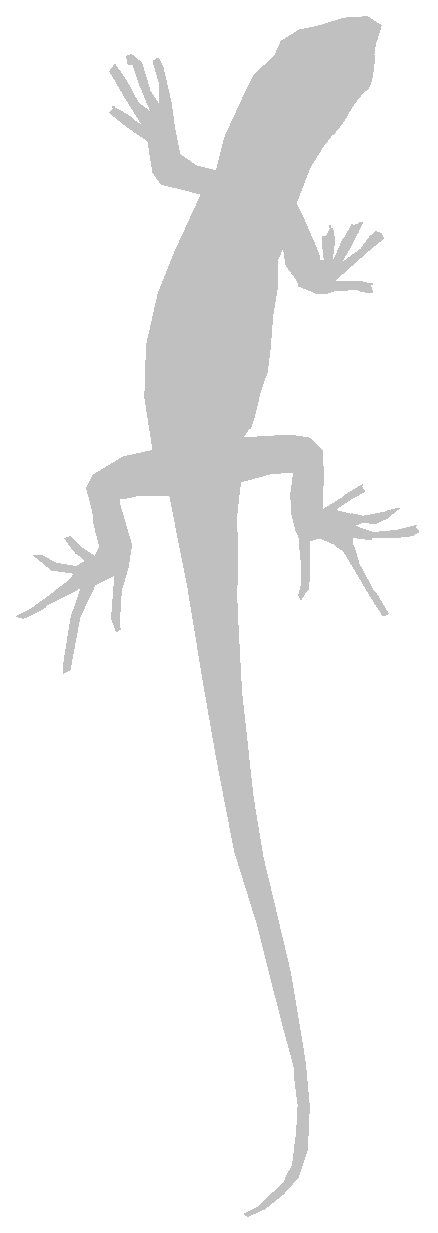
\includegraphics[width=0.1\textwidth,angle=270]{../../_common/fig/logo.eps}
\end{center}

\cleardoublepage

\vspace*{12cm}
\begin{tabular}{ll}
Author      & David Kneis \\
Affiliation & Institute of Earth and Environmental Sciences \\
            & Hydrology \& Climatology Section, \\
            & University of Potsdam, Germany \\
Contact     & david.kneis [at] uni-potsdam.de \\
            & \\
Project     & PROGRESS \\
Sub-project & D2.2 \\
Funding     & German Ministry of Education and Research (BMBF) \\
            & \\
Last update & \today{} \\
\end{tabular}

\vspace*{2.0cm}
\noindent Please help to improve this document by sending suggestions, corrections, wishes, and other useful feedback to the author (see above).

\cleardoublepage

%%%%%%%%%%%%%%%%%%%%%%%%%%%%%%%%%%%%%%%%%%%%%%%%%%%%%%%%%%
%%%%%%%%%%%%%%%%%%%%%% Page style   %%%%%%%%%%%%%%%%%%%%%%
%%%%%%%%%%%%%%%%%%%%%%%%%%%%%%%%%%%%%%%%%%%%%%%%%%%%%%%%%%

%%% Begin Fancy Header Settings
\pagestyle{fancy}                       % Sets fancy header and footer
\fancyfoot{}                            % Delete current footer settings
\renewcommand{\chaptermark}[1]{         % Lower Case Chapter marker style
  \markboth{\chaptername\ \thechapter\ \hspace{0.5cm} #1}{}}
\renewcommand{\sectionmark}[1]{         % Lower case Section marker style
  \markright{\thesection\ \hspace{0.5cm} #1}}
\fancyhead[LE,RO]{\bfseries\thepage}    % Page number (boldface) in left on even pages and right on odd pages
\fancyhead[RE]{\bfseries\leftmark}      % Chapter in the right on even pages
\fancyhead[LO]{\bfseries\rightmark}     % Section in the left on odd pages
\renewcommand{\headrulewidth}{0.3pt}    % Width of head rule %%% Clear Header
%% End Fancy Header Settings

%%%%%%%%%%%%%%%%%%%%%%%%%%%%%%%%%%%%%%%%%%%%%%%%%%%%%%%%%%
%%%%%%%%%%%%%%%%%%%%%% TOC          %%%%%%%%%%%%%%%%%%%%%%
%%%%%%%%%%%%%%%%%%%%%%%%%%%%%%%%%%%%%%%%%%%%%%%%%%%%%%%%%%

%% Begin TOC Settings
\pdfbookmark[1]{\contentsname}{toc}
\fancyhead[LE,RO]{\bfseries\thepage}
\fancyhead[RE]{\bfseries Contents}
\fancyhead[LO]{\bfseries Contents}
\tableofcontents
%% End TOC Settings

%%%%%%%%%%%%%%%%%%%%%%%%%%%%%%%%%%%%%%%%%%%%%%%%%%%%%%
%%%%%%%%%%%%%%%%%%%%%% ABSTACTS %%%%%%%%%%%%%%%%%%%%%%
%%%%%%%%%%%%%%%%%%%%%%%%%%%%%%%%%%%%%%%%%%%%%%%%%%%%%%

\onecolumn

% English summary
%\cleardoublepage
%\fancyhead[LE,RO]{\bfseries\thepage}
%\fancyhead[RE]{ }
%\fancyhead[LO]{ }
%\selectlanguage{american}
%\section*{Abstract}
\addcontentsline{toc}{chapter}{Abstract}

English abstract.



% German dummary
%\cleardoublepage
%\fancyhead[LE,RO]{\bfseries\thepage}
%\fancyhead[RE]{ }
%\fancyhead[LO]{ }
%\selectlanguage{ngerman}
%\section*{Kurzfassung}
\addcontentsline{toc}{chapter}{German abstract}

Deutsches Abstract.


%\selectlanguage{american}
%\cleardoublepage

%%%%%%%%%%%%%%%%%%%%%%%%%%%%%%%%%%%%%%%%%%%%%%%%%%%%%%%%%%
%%%%%%%%%%%%%%%%%%%%%% THE CHAPTERS %%%%%%%%%%%%%%%%%%%%%%
%%%%%%%%%%%%%%%%%%%%%%%%%%%%%%%%%%%%%%%%%%%%%%%%%%%%%%%%%%

\twocolumn

% Reestablish header
\fancyhead[LE,RO]{\bfseries\thepage}    % Page number (boldface) in left on even pages and right on odd pages
\fancyhead[RE]{\bfseries\leftmark}      % Chapter in the right on even pages
\fancyhead[LO]{\bfseries\rightmark}     % Section in the left on odd pages

%%%%% Chapter sources
\chapter{Introduction} \label{chap:intro}
\renewcommand{\tabdir}{chapters/intro/tab}
\renewcommand{\figdir}{chapters/intro/fig}

\section{The \software{echse} simulation environment} \label{sec:intro_idea}

The idea of a \emph{simulation environment}\index{simulation environment}\index{modeling framework|see{simulation environment}}\index{generic model|see{simulation environment}} is to provide a tool which can be used to simulate different systems and/or processes in a single unified software environment. Terms sometimes used more or less synonymously are \emph{modeling framework}, \emph{generic model} or \emph{open structure} model. Examples of existing modeling frameworks in the field of earth and environmental sciences include the \emph{Object Modeling System} \citep{Ahuja2005} and the \emph{Earth System Modeling Framework} \citep{Hill2004}. Examples from the field of water quality modeling include, for example, \emph{AQUASIM} \citep{Reichert1998}, the biogeochemical reactions network simulator BRNS \citep{Regnier2002, Thullner2005}, and the \emph{ECO Lab} software \citep{DHI2006}.

The benefit of a modeling framework usually emerges in situations, where
\begin{itemize}
  \item new models have to be developed in short time.
  \item a preliminary model has to be build and later improvement (possibly by different staff) is planned.
  \item alternative model structures are to be compared (to find an optimum structure or to learn about structural uncertainty).
  \item different people are involved in collaborative model development.
  \item a larger number of individual models must be used and a common (user) interface for all models is required (in operational forecasting, for example).
\end{itemize}

A basic characteristics of a modeling framework is the flexibility to simulate \emph{objects} of different \emph{classes} \footnote{An approximate synonym is \emph{types}.}. Typically, the features of a class, which include \emph{data} and \emph{methods} \footnote{An approximate synonym is \emph{functions}.} are declared/defined by the developer of a specific model for a specific purpose. In contrast to that, the generic core of the modeling framework represents the static part of the software, providing the basic infrastructure for all models (\figref{fig:intro-modelingFramework}).

\begin{figure}
  \centering
  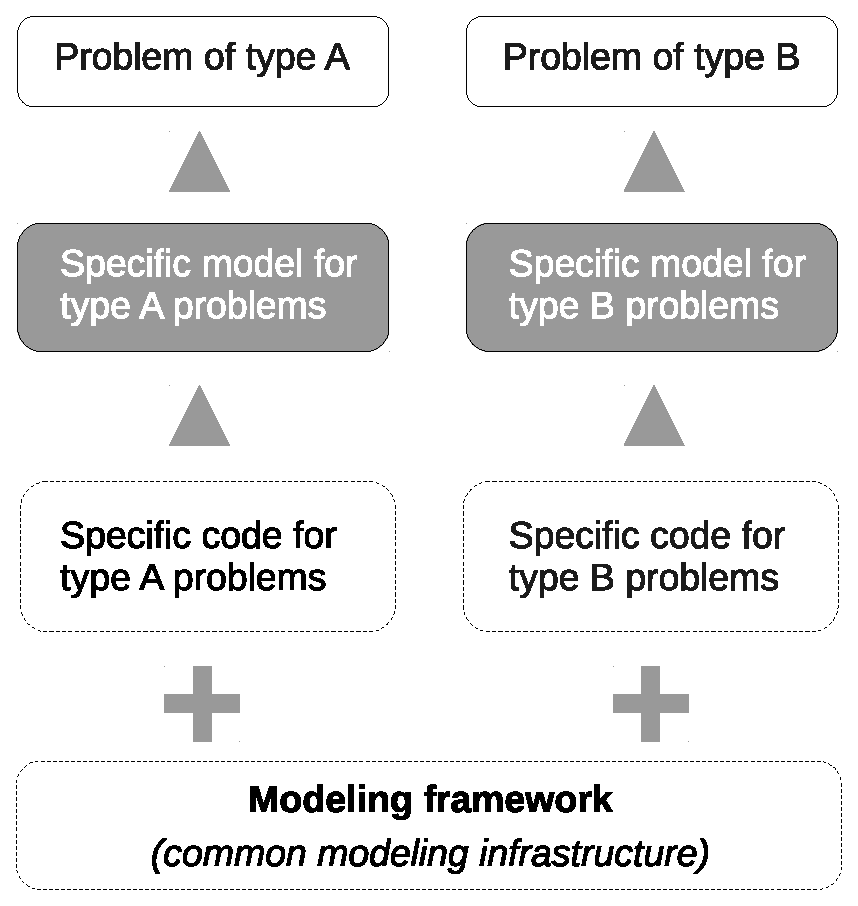
\includegraphics[width=0.9\columnwidth]{\figdir/modelingFramework.eps}
  \caption{Basic idea of a modeling framework. \label{fig:intro-modelingFramework}}
\end{figure}

The \software{echse}\index{\software{echse}} is intended to be a lightweight, simple to use modeling framework, being applicable to many (but not all) simulation problems, arising in the field of (eco)-hydrology. Details on potentials and limits are summarized in \secref{sec:intro_potentials-limits} and discussed in more detail in \chapref{chap:concept}.

It is important to understand that the \software{echse} simulation environment actually consists of two parts:
\begin{description}
  \item [The generic model core] This is a collection of source files. These files provide the common modeling intrastructure shown at the bottom of \figref{fig:intro-modelingFramework}.
  \item [The code generator] This is a software (currently implemented in R) to generate a large part of the \emph{application-specific} source code from basic information provided by the model developer. The generated source code is guaranteed to be compatible with the source code of the generic model core.
\end{description}

In order to create a specific model (grey boxes in \figref{fig:intro-modelingFramework}), the model developer finally has to complement the generated source code by implementing a set of methods (functions) with a simple, well defined interface. Only at this step, source code has to be written manually.

\section{Potential uses and limits} \label{sec:intro_potentials-limits}

Since the potential model applications in the field of eco-hydrology are so diverse, there is (and there cannot be) a modeling framework which is equally suitable for all those applications. Consequently, a 'good' modeling framework is usually one that is specialized on a certain range of applications (as opposed to a 'normal' model, that is specialized on a certain application alone).

The \software{echse} has been developed in the context of hydrological catchment modeling and water quality modeling. Therefore, this modeling framework is particularly specialized on
\begin{itemize}
  \item the simulation of a collection of objects representing instances of different classes (\eg{} catchments, river sections, lakes, etc.).
  \item the simulation of object interactions that are mostly of the \emph{feed-forward} type, \ie{} the simulated flow of mass, energy, or information is mostly unidirectional. \emph{Feedbacks}, \ie{} two-way interations between objects, may also be simulated but there are currently limitations with respect to the accuracy of results.
\end{itemize}

The current version of the \software{echse} is \emph{not} recommended for building models that
\begin{itemize}
  \item are dominated by feedback interactions between the simulated objects. That is, for example, the case in ground water or hydrodynamic modeling, where \emph{partial differential equations} (PDE) have to be solved. The concept of the \software{echse} currently does not support high-accuracy solutions of PDE.
  \item consist of a single object only. Simualting a single object is not a practical problem, but the use of other modeling tools may simply be more efficient.
\end{itemize}

\section{Required user skills} \label{sec:intro_skills}

\subsection{Use of existing models} \label{sec:intro_skills-use}

The skills required for using an existing model built with the \software{echse} are the same as for any other dynamic system model. You basically need to
\begin{itemize}
  \item understand the characteristics of the implemented classes (from a documentation of the specific model).
  \item know which input files are required (see \chapref{chap:input}).
  \item be able to create all input files. This can be done manually (for small projects only), by writing skripts (for example using R, Matlab, Python, etc.), and/or by using other programs such as spreadsheet software, geographical information systems, or data bases.
  \item understand the limits of the implemented model with respect to your specific application.
\end{itemize}

\subsection{Development of models} \label{sec:intro_skills-dev}

As with all modeling frameworks, the \software{echse} aims at reducing the effort for building new models and for changing/extending existing ones. Thus, you don't need to be a professional code writer. However, to successfully create or modify models, you should
\begin{itemize}
  \item understand the meaning of the terms 'class' and 'object' (see any introduction on object-oriented programming),
  \item know the different features of a class supported by \software{echse} and understand the meaning of the classes' 'simulate' methods (see \chapref{chap:concept}),
  \item have basic knowledge of ordinary differential equations and their use in the simulation of dynamic systems,
  \item be able to program simple algorithms in any language,
  \item be willing to get familiar with the most basic elements of C++ (basic data types, operators, and flow-control) or find someone who will translate (or wrap) your code if written in another language.
\end{itemize}

\chapter{Basic concepts} \label{chap:concept}
\renewcommand{\tabdir}{chapters/concept/tab}
\renewcommand{\figdir}{chapters/concept/fig}

%%%%%%%%%%%%%%%%%%%%%%%%%%%%%%%%%%%%%%%%%%%%%%%%%%%%%%%%%%%%%%%%%%%%%%%%%%%%%%%%
%%%%%%%%%%%%%%%%%%%%%%%%%%%%%%%%%%%%%%%%%%%%%%%%%%%%%%%%%%%%%%%%%%%%%%%%%%%%%%%%
%%%%%%%%%%%%%%%%%%%%%%%%%%%%%%%%%%%%%%%%%%%%%%%%%%%%%%%%%%%%%%%%%%%%%%%%%%%%%%%%
\section{Important terms} \label{sec:concept-terms}

To understand the concept behind all models created with the \software{echse} simulation environment, one must know the meaning of the terms \emph{class}, \emph{object}, and \emph{object group}. These terms are defined in the following sections (see also  \figref{fig:concept-terms}).

\subsection{Objects} \label{sec:concept-terms-objects}

Objects\index{object!definition} are the basic building blocks of any model created with the \software{echse} simulation environment. An object in the model typically represents a real-world object (such as a tree, a lake, a soil column, etc.). Usually, the object in the model is a simplified, abstract description of the corresponding real-world object, \ie{} it describes only its most important characteristics (for example height, average diameter, and age of a tree). However, an objects does \emph{not necessarily} correspond to an entity existing in the real-world. For example, the function of such a more abstract object may be to simply collect information on some other objects and to supply this information to a third object (like a kind of observer).

Technically speaking, an object always represents an instance of an underlying class (see \secref{sec:concept-terms-classes}). For example, a single tree object is an instance of the tree class. In a typical model, (1) there are multiple instances of the \emph{same} class (such as multiple trees) and (2) multiple objects of \emph{different} classes do co-exist (such as trees and lakes).

The basic features of an object, \ie{} the information and functionality linked to that object, are always determined by the corresponding class (a tree has a diameter and may grow, a lake has a depth and its storage may change). The general features of classes are described in \secref{sec:concept-classFeatures}.

In a typical model, the objects (no matter, of which class) do interact in some way. These interactions typically represent the exchange of matter, energy, or information between the corresponding real-world entities. For example, two lakes could exchange water via a connecting channel or the growth of a tree might depend on a lake's water level.

The collection of all interacting objects is typically called the \emph{model}.

\subsection{Classes} \label{sec:concept-terms-classes}

A class\index{class!definition} represents an abstract prototype for a certain type of object (\emph{type} is an approximate synonym for \emph{class}). A class describes the features of \emph{all} objects that are instances of that particular class. In the language of object-oriented programming, the features of a class are typically called 'class members'. Such member either represent data (\ie{} information) or methods (\ie{} algorithms, describing the functionality of an object of that class). For example, a class 'lake' might have the water level, the storage volume, and the geo-coordinates of its center as data members. These data members (not to be confused with the actual values) are then common to all instances of the class, \ie{} all lake objects.

Generally, a class is distinguished from other classes by
\begin{itemize}
  \item its data members (for example, the number and names of state variables) and/or,
  \item its methods. In the context of the \software{echse}, each class has only a single visible method called 'simulate'. This method typically describes the dynamics of the class' state variables.
\end{itemize}

The members of classes are introduced in detail in \secref{sec:concept-classFeatures}.

\subsection{Object groups} \label{sec:concept-terms-objectgroups}

The term object group\index{object group} is used for all instances (\ie{} objects) of a particular class. If a forest of individual trees is modeled, for example, all trees belong to the same object group. Though, in many instances, the terms \emph{class} and \emph{object group} are (and can be) used synonymously, they are not actually interchangeable:
\begin{description}
  \item [A class] is the prototype of all objects with the same data and functionality.
  \item [An object group] represents the array of all objects (\ie{} instances) of a particular class.
\end{description}

\subsection{Summary} \label{sec:concept-terms-summary}

The relation between the terms \emph{class}, \emph{object}, \emph{object group}, and \emph{model} is illustrated with an example in \figref{fig:concept-terms}. Another view on the relations between these terms is provided in \figref{fig:concept-terms_implementation}. This figure is intended for those who are familiar with basic techniques of object-oriented programming. Shown are 8 objects, which belong to 2 different classes 'A' and 'B'. All these 8 objects inherit from an abstract base class 'abstractObject'. It is therefore possible to keep handles to all these objects (of different classes) in a single array by using base-class pointers (\ie{} by treating them as objects of the base class). In the same way, handles to all object groups can be stored in a single array since they all inherit from an abstract base class 'abstractObjectGroup'. In each object group, an arbitrary number of objects may be declared. In contrast to that, only a single instance of each object group can exist.


\begin{figure}
  \centering
  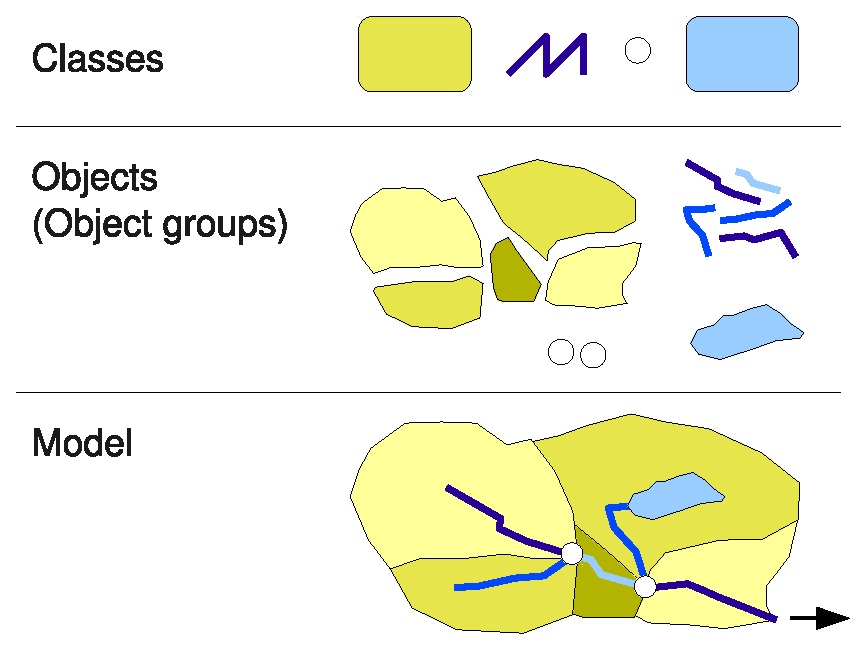
\includegraphics[width=0.9\columnwidth]{\figdir/terms_class-object-objGroup/terms_class-object-objGroup.eps}
  \caption[Relation between the terms \emph{class}, \emph{object}, \emph{object group}, and \emph{model}.]{Relation between the terms \emph{class}, \emph{object}, \emph{object group}, and \emph{model} with the example of a hydrological catchment model, consisting of sub-catchments (green polygons), river reaches (blue lines), lakes (blue polygons), and river nodes (circles). \label{fig:concept-terms}}
\end{figure}

\begin{figure}
  \centering
  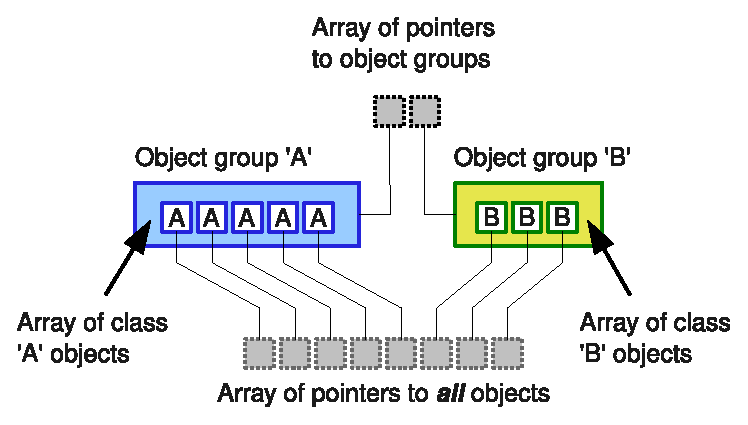
\includegraphics[width=0.9\columnwidth]{\figdir/terms_class-object-objGroup/terms_class-object-objGroup_implementation.eps}
  \caption[\emph{Classes}, \emph{objects}, and \emph{object groups} from a programmers point of view.]{\emph{Classes}, \emph{objects}, and \emph{object groups} from a programmers point of view. \label{fig:concept-terms_implementation}}
\end{figure}

\FloatBarrier

%%%%%%%%%%%%%%%%%%%%%%%%%%%%%%%%%%%%%%%%%%%%%%%%%%%%%%%%%%%%%%%%%%%%%%%%%%%%%%%%
%%%%%%%%%%%%%%%%%%%%%%%%%%%%%%%%%%%%%%%%%%%%%%%%%%%%%%%%%%%%%%%%%%%%%%%%%%%%%%%%
%%%%%%%%%%%%%%%%%%%%%%%%%%%%%%%%%%%%%%%%%%%%%%%%%%%%%%%%%%%%%%%%%%%%%%%%%%%%%%%%
\section{Features (members) of a class} \label{sec:concept-classFeatures}

%%%%%%%%%%%%%%%%%%%%%%%%%%%%%%%%%%%%%%%%%%%%%%%%%%%%%%%%%%%%%%%%%%%%%%%%%%%%%%%%
%%%%%%%%%%%%%%%%%%%%%%%%%%%%%%%%%%%%%%%%%%%%%%%%%%%%%%%%%%%%%%%%%%%%%%%%%%%%%%%%
\subsection{Overview} \label{sec:concept-classFeatures-overview}

An overview of the features (precisely: members\index{class!members}) of a class is given in \figref{fig:concept-classFeatures-overview}. Details on the data members are provided first in \secsref{sec:concept-classFeatures-states} to \ref{sec:concept-classFeatures-outputs}. The 'simulate' method, which is the most important member function of a class, is addressed in \ref{sec:concept-classFeatures-simulateMethod}.

\begin{figure}
  \centering
  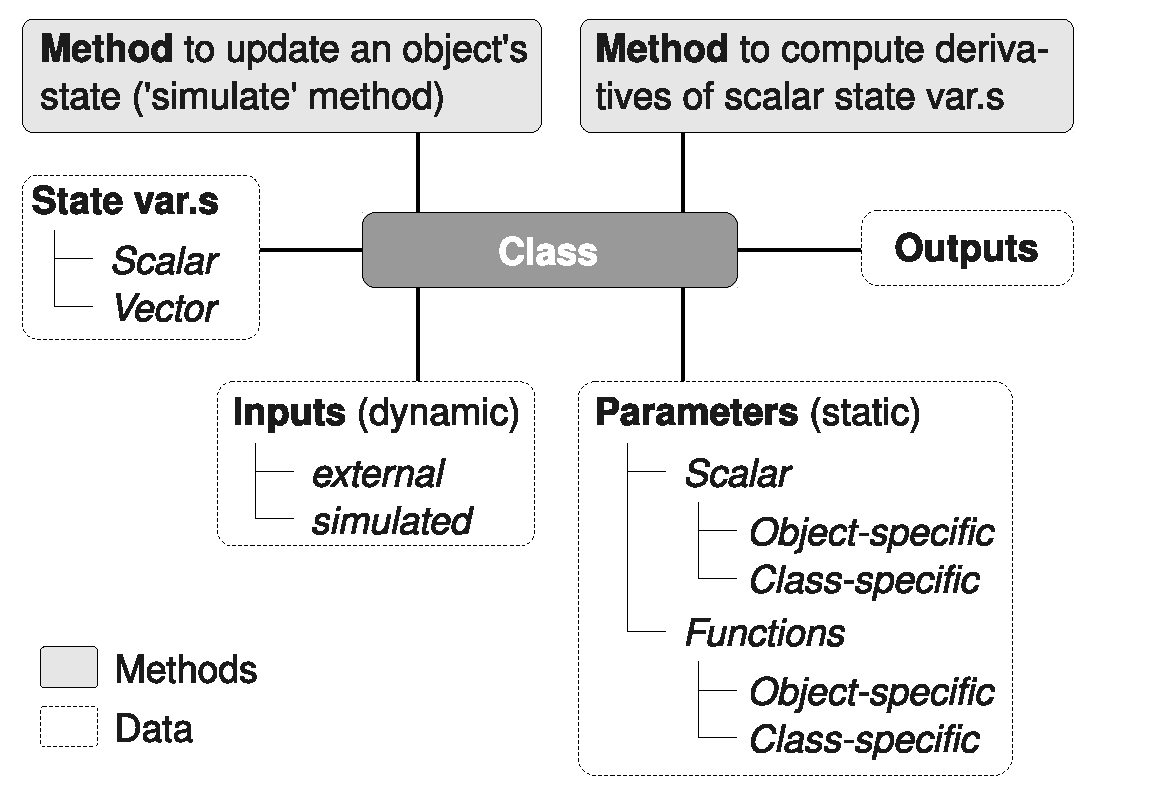
\includegraphics[width=0.9\columnwidth]{\figdir/classFeatures/classFeatures.eps}
  \caption[Overview of the features of a class.]{Overview of the features (members) of a class. The dashed line separates data members (below) from class methods (above line). \label{fig:concept-classFeatures-overview}}
\end{figure}

%%%%%%%%%%%%%%%%%%%%%%%%%%%%%%%%%%%%%%%%%%%%%%%%%%%%%%%%%%%%%%%%%%%%%%%%%%%%%%%%
%%%%%%%%%%%%%%%%%%%%%%%%%%%%%%%%%%%%%%%%%%%%%%%%%%%%%%%%%%%%%%%%%%%%%%%%%%%%%%%%
\subsection{State variables} \label{sec:concept-classFeatures-states}

State variables\index{state variable} describe the state of an object at a certain point in time. State variables are dynamic data, \ie{} their values may change over time. Consequently, at the start of a simulation, their values must be initialized. In \software{echse}-based models, a class may contain both single-valued (scalar) and vector-valued state variables.

\subsubsection*{Scalar state variables} \label{sec:concept-classFeatures-statesScal}

\emph{Scalar state variables}\index{state variable!scalar} are state variables that take a single value only. Looking at a reservoir, for example, the storage volume is a scalar state variables, since it can be expressed as a single number. In contrast to that, the reservoirs' water depth (as it is spatially variable) is not a scalar variable by nature. The average depth, however, may be treated as a scalar state variable.

\subsubsection*{Vector state variables} \label{sec:concept-classFeatures-statesVect}

In contrast to a scalar state variables, \emph{vector state variables}\index{state variable!vector-valued} are vector-valued, \ie{} their value(s) cannot be adequately expressed by a single number. For example, a vector state variable may be required to adequately describe the temperature in a deep reservoir. Due to stratification, there are often significant vertical temperature gradients which often cannot be (convieniently) described by a single value (\ie{} a scalar state variable). Another example of a vector state variable is the water level of a river reach, measured at multiple stations along that reach.

%%%%%%%%%%%%%%%%%%%%%%%%%%%%%%%%%%%%%%%%%%%%%%%%%%%%%%%%%%%%%%%%%%%%%%%%%%%%%%%%
%%%%%%%%%%%%%%%%%%%%%%%%%%%%%%%%%%%%%%%%%%%%%%%%%%%%%%%%%%%%%%%%%%%%%%%%%%%%%%%%
\subsection{Input variables} \label{sec:concept-classFeatures-inputs}

Input variables (also called forcings)\index{input variable} represent time-variable data, representing the dynamic environment of an object. Typically, changes in the values of an object's state variables are triggered by changes in the input variables. In \software{echse} models, \emph{external} and \emph{simulated} (synonym: internal) inputs are distinguished.

%%%%%%%%%%%%%%%%%%%%%%%%%%%%%%%%%%%%%%%%%%%%%%%%%%%%%%%%%%%%%%%%%%%%%%%%%%%%%%%%
\subsubsection*{External inputs} \label{sec:concept-classFeatures-inputsExt}

External input variables\index{external input}\index{input variable!external|see{external input}}\index{forcing|see{external input}}\index{boundary condition|see{external input}} are variables, whose dynamics is \emph{not} simulated by the model. Instead, the dynamics is prescribed, \ie{} the values must be known in advance for the entire modeling period. The model reads those data from time series files (see \secref{sec:input-external}). When simulating the temperature of a reservoir, for example, solar radiation and air temperature are typically external input variables (since the atmosphere itself is not part of the model). Values of the external input variables usually represent observations (when simulating the past). In the context of forecasting, the values often originate from forecasts which have been produced by an external model. For example, a hydrological model for medium-term stream flow forecasting uses the forecasts produced by a numerical weather prediction model as input.

%%%%%%%%%%%%%%%%%%%%%%%%%%%%%%%%%%%%%%%%%%%%%%%%%%%%%%%%%%%%%%%%%%%%%%%%%%%%%%%%
\subsubsection*{Simulated inputs} \label{sec:concept-classFeatures-inputsSim}

The values of simulated input variables\index{simulated input}\index{input variable!simulated|see{simulated input}} are computed \emph{within} the model itself. From the perspective of an object, a simulated input variable is a variable, whose values are supplied by another object, \ie{} the existence of such variables is bound to interactions between objects. More precisely, a simulated input variable of an object 'A' is always linked to an output variable (see \secref{sec:concept-classFeatures-outputs}) of another object 'B'. This is due to the fact that only the output variables of an object are visible to (and accessible by) other objects. A typical example for the use of simulated inputs is the 'reservoir' class in a hydrological model. From the perspective of a reservoir, the inflow is a simulated input variable, if the values are supplied by an upstream object. The corresponding output variable of the upstream object is usually an outflow rate (of a reach) or a runoff rate (from the reservoir's catchment).

%%%%%%%%%%%%%%%%%%%%%%%%%%%%%%%%%%%%%%%%%%%%%%%%%%%%%%%%%%%%%%%%%%%%%%%%%%%%%%%%
%%%%%%%%%%%%%%%%%%%%%%%%%%%%%%%%%%%%%%%%%%%%%%%%%%%%%%%%%%%%%%%%%%%%%%%%%%%%%%%%
\subsection{Parameters} \label{sec:concept-classFeatures-params}

Those properties of an object which are static (\ie{} which do not change over time), are called \emph{parameters}\index{parameter}. As outlined in \figref{fig:concept-classFeatures-overview}, different kinds of parameters are supported by the \software{echse}. These are described in detail in the subsequent sections.

%%%%%%%%%%%%%%%%%%%%%%%%%%%%%%%%%%%%%%%%%%%%%%%%%%%%%%%%%%%%%%%%%%%%%%%%%%%%%%%%
\subsubsection*{Scalar parameters} \label{sec:concept-classFeatures-paramsNum}

\emph{Scalar parameters}\index{parameter!scalar} are, like scalar state variables, characterized by the fact that they are single-valued. Thus, the value of a scalar parameter is always just a single number. In the \software{echse}, two types of scalar parameters are distinguished:
\begin{description}
  \item [Object-specific scalar parameters]: The value of these parameters are specific for a particular object (of a particular class). For example, a 'catchment' class could have an object-specific scalar parameter 'area'. Then, values of the area may be assigned to each catchment object individually.
  \item [Group-specific scalar parameters]: The value of such a parameter cannot be set for individual objects. Instead, a common value is assigned to \emph{all} objects of a particular class. For example, in a 'catchment' class, the long-wave emissivity of the snow cover could be declared as a group-specific scalar parameter, if a common value for all modeled catchments is appropriate.
\end{description}

Note: Hard-coded scalar parameters, \ie{} the definition of constants in the 'simulate' method of a class, provide(s) an alternative to group-specific scalar parameters. The use of hard-coded parameters is preferable \emph{only} if it is known that the values are strictly constant. This is typically the case for physical constants with a well known value (such as the specific heat capacity of water). The drawback of using hard-coded parameters is that any modification of the values requires the source code to be re-compiled. Note that, strictly speaking, such hard-coded parameters are not \emph{data members} of the class and, therefore, they do not show up in \figref{fig:concept-classFeatures-overview}.

%%%%%%%%%%%%%%%%%%%%%%%%%%%%%%%%%%%%%%%%%%%%%%%%%%%%%%%%%%%%%%%%%%%%%%%%%%%%%%%%
\subsubsection*{Parameter functions} \label{sec:concept-classFeatures-paramsFun}

In many situations, some static object properites need to be represented by functions\index{parameter!function} instead of scalar parameters. An example is the relationships between water depth and storage volume in a river reach or lake. The \software{echse} basically supports two concepts of functions:
\begin{enumerate}
  \item Tabulated functions (synonym: lookup tables).
  \item Analytical expressions.
\end{enumerate}

\paragraph{Tabulated functions:} Lookup tables provide a means to describe also those functional relations between two entities which cannot be reasonably captured by an analytical expression. Although, in many cases, a piecewise polynomial representation might be possible, lookup tables offer a more flexible and convenient alternative. The \software{echse} supports tabulated functions as long they have a single argument only. There is support for both functions with regular (\ie{} equally spaced) arguments and functions with non-regular arguments. Like in the case of scalar parameters, two types of such lookup-based parameter functions may be distinguished:

\begin{description}
  \item [Object-specific parameter functions]: This type of function is object-specific, \ie{} an individual lookup table is assigned to each object (of a particular class). For example, the rating curve might be declared as an object-specific parameter function in a 'gage' class, since each gage has its own characteristic rating curve.
  \item [Group-specific parameter functions]: Such a function is not associated with an individual object. Instead, it represents a common function which is accessible to all objects (of a particular class).
\end{description}

\paragraph{Analytical expressions:} If a function can be captured by a single (or few) analytical expression(s), then it is typically hard-coded, \ie{} the function is defined in the 'simulate' method of a class. It is then, strictly speaking, not a \emph{data member} of the class and, therefore, hard-coded functions do not show up in \figref{fig:concept-classFeatures-overview}. Hard-coded analytical functions include, for example, polynomials, and linear, exponential, or power functions. The advantage of using them is that the function's return value may usually be computed more quickly as compared to table-lookup.

A typical case of an analytical function that one would hard-code is the Magnus-Formula, which is is an empirical expression relating the air's maximum humidity to air temperature. It is an example of a function which is \emph{not} object-specific since it is practically applicable everywhere on earth.

However, it is quite straightforward to make hard-coded functions object-specific. This is simply achieved by passing the coefficients of analytical expressions via the functions interface and to define those coefficients as object-specific \emph{scalar parameters}. For example, a rating curve may sometimes be expressed by a power expression like $Q=a \cdot H^b$, with $a$ and $b$ being empirical coefficients and $Q$ and $H$ representing discharge and stage, respectively. In such a case, one may declare $a$ and $b$ as object-specific \emph{scalar} parameters in a 'gage' class to let each gages have its individual rating curve.

Note that hard-coded analytical functions provide the only way of implementing functions that take multiple variable arguments (multi-dimensional functions). This is due to the fact that there is currently no support for multi-dimensional table lookup. In some situations, however, it may be possible to split a multi-dimensional function into several single-argument functions which may then be represented by lookup tables.

%%%%%%%%%%%%%%%%%%%%%%%%%%%%%%%%%%%%%%%%%%%%%%%%%%%%%%%%%%%%%%%%%%%%%%%%%%%%%%%%
%%%%%%%%%%%%%%%%%%%%%%%%%%%%%%%%%%%%%%%%%%%%%%%%%%%%%%%%%%%%%%%%%%%%%%%%%%%%%%%%
\subsection{Output variables} \label{sec:concept-classFeatures-outputs}

To make information about an object visible to (and usable for) its environment, \emph{output variables}\index{output variable} must be declared in the respective class. In particular, output variables have to be declared in a class for all data, which
\begin{itemize}
  \item should to be passed from an object of that class to another simulated object.
  \item are of interest to the modeler and should (potentially) be available in the output files.
\end{itemize}

In a hydrological catchment model, for example, a 'catchment' class might have an output variable 'runoff'. Then, the values of that variable may serve as an input to an object of class 'reach', for example, provided that a corresponding \emph{simulated input} variable (see \secref{sec:concept-classFeatures-inputsSim}) exists in the 'reach' class. Furthermore, the existance of the output variable 'runoff' allows for writing the computed runoff for user-selected catchments to the respective output files.

In each class, at least a single output variable should be defined because objects of that class are otherwise useless. Typically, output variables are used to retrieve information on
\begin{itemize}
  \item state variables.
  \item flux rates, such as time-step averages of energy or mass fluxes.
\end{itemize}
However, there are practically no limitations, \ie{} any scalar value which is computed (or which is accessible) in the 'simulate' method of a class (see \secref{sec:concept-classFeatures-simulateMethod}) can be assigned to an output variable.

%%%%%%%%%%%%%%%%%%%%%%%%%%%%%%%%%%%%%%%%%%%%%%%%%%%%%%%%%%%%%%%%%%%%%%%%%%%%%%%%
%%%%%%%%%%%%%%%%%%%%%%%%%%%%%%%%%%%%%%%%%%%%%%%%%%%%%%%%%%%%%%%%%%%%%%%%%%%%%%%%
\subsection{The 'simulate' method} \label{sec:concept-classFeatures-simulateMethod}

\subsubsection*{Purpose and interface}
The 'simulate' method\index{simulate method} of a class represents the class' most important member function which needs to be defined by the model developer.

The purpose of the 'simulate' method is to simulate the evolution of an object over a period of length $\Delta t$. This is usually equivalent to solving a so-called \emph{initial value problem} which means that

\begin{enumerate}
  \item the values of the object's $n$ state variables at an initial time $t_0$ are known.
  \item the values at time $t_0 + \Delta t$ are to be computed by integrating $n$ ordinary differential equations (one ODE per state variable).
\end{enumerate}

Thus, the 'simulate' method usually implements a solution of the initial value problem. The ordinary differential equations (ODEs) to be solved are specific for each class and they typically describe either a mass or energy balance (see example in \secref{sec:concept-classDef}). Whether the integration can be performed using simple approaches (such as a first order Euler method) or whether sophisticated ODE solvers \citep[see \eg{}][]{Press2002} are required, depends on the specific problem. In addition to the updating of state variables, the 'simulation' method is responsible for calculating all auxiliary numeric data, which are of interest to the model user, \ie{} model outputs (see \secref{sec:concept-classFeatures-outputs}).

In C++ notation, the interface of the 'simulate' method looks like

\medskip
{\small \verb!.simulate(const unsigned int delta_t)!}
\medskip

where \verb!delta_t! is the function's (only) argument. It is of type unsigned integer and represents the simulation time step in seconds. Note that no other information are passed via the function's argument list.

\subsubsection*{Class-specific behavior}
The leading dot in the function's name (see interface above) indicates that this function is a class member. Formally speaking, it is a \emph{virtual} member of the \emph{abstract} class 'abstractObject' describing a generic object (\figref{fig:concept-simulateMethod}). The child classes describing a specific type of (usually real-world) objects are derived from that abstract parent class. Through the mechanisms of inheritance, each child class automatically has a 'simulate' method with the interface shown above. Although the function's name is the same, the interior of the method is \emph{class-specific}, since the implementation is only present in the child classes but not in the base class (\figref{fig:concept-simulateMethod}). This makes it possible to use identical calls like

\medskip
{\small \verb!reservoir_xy.simulate(3600)!}

{\small \verb!catchment_288.simulate(3600)!}
\medskip

to trigger the simulation of two objects, which are instances of \emph{different} classes (a 'reservoir' and a 'catchment', in this example). The appropriate code for each object is selected automatically at run-time, based on the type information.

\begin{figure*}[htb]
\lstinputlisting[style=c++]{\figdir/simulate-methods/simulate-methods.txt}
  \caption[Specification of the 'simulate' methods in the abstract base class (parent class) and the application-specific child classes.]{Specification of the 'simulate' methods in the abstract base class (parent class) and the application-specific child classes. Only relevant parts of the C++ code of the classes are shown. \label{fig:concept-simulateMethod}}
\end{figure*}

\subsubsection*{Access to an object's data}

As mentioned earlier, the time step \verb!delta_t! is the only information passed to the 'simulate' method via the argument list. All object-related data, such as the values of parameters, inputs, and state variables, are available through class methods. These methods, which may also be called \emph{data access methods}, are summarized in \tabsref{tab:concept-dataAccessFunctions_read} and \ref{tab:concept-dataAccessFunctions_write}.

The read-only methods (\tabref{tab:concept-dataAccessFunctions_read}) are intended for retrieving information. They can appear at the right-hand side of assignments and the methods with a scalar result type may be used in mathematical expressions or comparisons just like normal variables of type \verb!double!. The method for retrieving the values of a vector state variable does not return a scalar result but a constant reference to a numeric vector (\verb!const vector <double> &!). Note that it depends on the \emph{usage} of the return value whether a copy of the retrieved data is generated or not. This is important in terms of computational efficiency if the vectors are large size. To avoid the creation of a copy, you have to use the returned value to initialize a const reference. In C++, this would look like

\medskip
\begin{footnotesize}
  \verb!const vector <double> & = stateVect(name);!
\end{footnotesize}
\medskip

where \verb!name! is the name of the respective vector state variable. If you assign the return value to a 'normal' variable, \ie{} a non-constant numeric vector which is not a reference, using

\medskip
\begin{footnotesize}
  \verb!vector <double> = stateVect(name);!
\end{footnotesize}
\medskip

a copy of the data will be created. Note that this distinction is also relevant when passing the vector to a function via the function's argument list. Since you often want to pass a constant reference instead of a copy of the values, the dummy argument should be declared accordingly.

The purpose of the write-only methods (\tabref{tab:concept-dataAccessFunctions_write}) is to assign new values to an object's state or output variables (see example in \secref{sec:concept-classDef}). The write-only methods all return non-const references to scalars or vectors. These methods typically appear at the left-hand side of assignment statements. They may also be used as actual parameters in function calls, if the corresponding template parameter is a non-const reference of the appropriate type (\ie{} the parameter represents an output of the function).

\begin{table*}[htb]
  \caption[Data access methods, part I: Read-only methods.]{Data access methods, part I: Read-only methods. The dummy argument \texttt{name}, has to be substituted by the name of the particular variable, parameter, or function to be accessed. The names are defined by the model developer. Note that names must not be quoted since they do not represent strings but (automatically defined) index constant. For the dummy argument \texttt{arg}, a numeric expression representing the function's argument has to be supplied. \label{tab:concept-dataAccessFunctions_read}}
  \begin{tabular}{p{0.18\textwidth}ll} \hline\hline
    Type of feature       & Call                   & Result type \\ \hline
    Scalar state variable & \verb!stateScal(name)! & \verb!double! \\
    Vector of scalar state variables & \verb!stateScal_all()! & \verb!const vector <double> &! \\
    Vector state variable & \verb!stateVect(name)! & \verb!const vector <double> &! \\
    External input    & \verb!inputExt(name)! & \verb!double! \\
    Simulated input   & \verb!inputSim(name)! & \verb!double! \\
    Parameter function (object-specific) & \verb!paramFun(name, arg)! & \verb!double! \\
    Scalar parameter (object-specific) & \verb!paramNum(name)! & \verb!double! \\
    Parameter function (group-specific) & \verb!sharedParamFun(name, arg)! & \verb!double! \\
    Scalar parameter (group-specific) & \verb!sharedParamNum(name)! & \verb!double! \\
    \hline\hline
  \end{tabular}
\end{table*}

\begin{table*}[htb]
  \caption[Data access methods, part II: Write-only methods.]{Data access methods, part II: Write-only methods. See \tabref{tab:concept-dataAccessFunctions_read} for details on the methods' \texttt{name} argument. \label{tab:concept-dataAccessFunctions_write}}
  \begin{tabular}{p{0.3\textwidth}ll} \hline\hline
    Type of feature & Call & Assigned type \\ \hline
    Scalar state variable & \verb!set_stateScal(name)! & \verb!double &! \\
    Vector of scalar state variables & \verb!set_stateScal_all()! & \verb!vector <double> &! \\
    Vector state variable & \verb!set_stateVect(name)! & \verb!vector <double> &! \\
    Output variable & \verb!set_output(name)! & \verb!double &! \\
    \hline\hline
  \end{tabular}
\end{table*}

\subsubsection*{Mandatory actions}
According to the purpose of the 'simulate' method (see above), there is a minimum set of statements that should be present in this method for every class (see example in \secref{sec:concept-classDef}). In particular, the method should contain
\begin{enumerate}
  \item statements to update the values of all state variables using the method(s) from row 1 \& 2 of \tabref{tab:concept-dataAccessFunctions_write}. As discussed earlier, this usually means that ordinary differential equations are solved (see also \secref{sec:concept-classFeatures-derivsScal}).
  \item statements to set the values of all output variables (see last row of \tabref{tab:concept-dataAccessFunctions_write}).
\end{enumerate}

%%%%%%%%%%%%%%%%%%%%%%%%%%%%%%%%%%%%%%%%%%%%%%%%%%%%%%%%%%%%%%%%%%%%%%%%%%%%%%%%
%%%%%%%%%%%%%%%%%%%%%%%%%%%%%%%%%%%%%%%%%%%%%%%%%%%%%%%%%%%%%%%%%%%%%%%%%%%%%%%%
\subsection{The 'derivsScal' method} \label{sec:concept-classFeatures-derivsScal}
As described in \secref{sec:concept-classFeatures-simulateMethod}, the purpose of the 'simulate' method is usually to integrate a single (or a set of) ordinary differential equation(s) over time. In some situations, the use of a simple first-order approximation (Euler's method) may be sufficient. Such methods, however, are neither accurate nor stable. If more accurate and stable solutions are needed, an ODE solver must be used which yields higher-order estimates and automatically adjusts the size of time (sub)steps.

The \software{echse} comes with a built-in ODE solver based on the 5-th order Runge-Kutta method described in \citet{Press2002}. This is a quite robust algorithm. However, its applicability is restricted to \emph{non-stiff} systems of simultaneous ODE. This may be relevant if the number of state variables of an object is > 1.

As with all ODE solvers, one must pass a method to the solver which computes the derivatives of the state variables (with respect to time, here). The name of the corresponding class method is 'derivsScal'. Like 'simulate', it is a virtual method. As the method's name indicates, it computes the derivatives of the scalar state variables only (see \secref{sec:concept-classFeatures-statesScal}). ODE solver support for vector state variables is currently not implemented.

The interface of the 'derivsScal' method is shown in \figref{fig:concept-classDef-methodsFrame}. The meaning of the dummy arguments is as follows:

\begin{tabular}{lp{0.8\columnwidth}}
  \verb!t! & This scalar \emph{input} argument represents the time. It is only relevant when simulating non-autonomous systems, \ie{} if the value(s) of the derivative(s) are time-depend. Note that this is only the case, if the forcings are variable within a time step. In many models, the forcings are treated as constant within a time step and the value of \verb!t! is not used in computing the derivatives. \\
  \verb!u! & \emph{Input} vector holding the values of the state variables whose derivatives are to be computed. \\
  \verb!dtdt! & \emph{Output} vector, containing the derivatives corresponding to the state variables in \verb!u!. \\
  \verb!delta_t! & \emph{Input} value, representing the length of the simulation time step. The intention of this argument is to allow for unit conversions. For example, external forcings (precipitation, radiation) may be given as sum values for a time step (mm/time step or J/\sqm{}/time step, for example). When computing the derivatives, such values need to be converted into rates (m/s or W/\sqm{}, for example) using the value of \verb!delta_t!. \\
\end{tabular}

In order to actually use this method, the code for computing the derivatives needs to provided in a separate file (see \verb!#include! directive in the 'derivsScal' method in \figref{fig:concept-classDef-methodsFrame}). This file must contain code which assigns a value to all elements of vector \verb!dudt!. At the right hand side of these assignments, one can use the access functions listed in \tabref{tab:concept-dataAccessFunctions_read} with one \emph{important exception}: One \emph{cannot} call the function \verb!stateScal! to access the value(s) of scalar state variable(s)! Instead, one must use the respective element of the input vector \verb!u! (appropriate constants for accessing a particular element are provided in the generated class header). This is because of the fact that the ODE solver internally computes derivatives for various estimates of the state variables' values. These estimates are passed in vector \verb!u!. Note that the body of the 'derivsScal' method can remain empty if there is no need for it (because the ODE(s) can be solved analytically, for example).

See \secref{sec:concept-classDef-simulate} for an example showing an implementation of the 'derivsScal' method and the use of the built-in ODE solver in the 'simulate' method.

%%%%%%%%%%%%%%%%%%%%%%%%%%%%%%%%%%%%%%%%%%%%%%%%%%%%%%%%%%%%%%%%%%%%%%%%%%%%%%%%
%%%%%%%%%%%%%%%%%%%%%%%%%%%%%%%%%%%%%%%%%%%%%%%%%%%%%%%%%%%%%%%%%%%%%%%%%%%%%%%%
%%%%%%%%%%%%%%%%%%%%%%%%%%%%%%%%%%%%%%%%%%%%%%%%%%%%%%%%%%%%%%%%%%%%%%%%%%%%%%%%

\FloatBarrier

\section{Automatic code generation} \label{sec:concept-autocode}

\subsection{Role of generated code in the \software{echse} framework} \label{sec:concept-autocode-role}
As stated in \chapref{chap:intro}, the \software{echse} is a generic modeling framework. As such, it consists of a generic, re-usable model core complemented by problem-specific extensions. The generic model core provides basic infrastructure for \emph{any} dynamic simulation model. The problem-specific extensions are required to build simulation models for a particular (type of) system.

In the case of the \software{echse} modeling framework, problem-specific extensions are equivalent to user-defined classes with the features described in \secref{sec:concept-classFeatures}. The relation between the generic model core and the problem-specific extensions is illustrated in \figref{fig:concept-autocode-role}.

\begin{figure}
  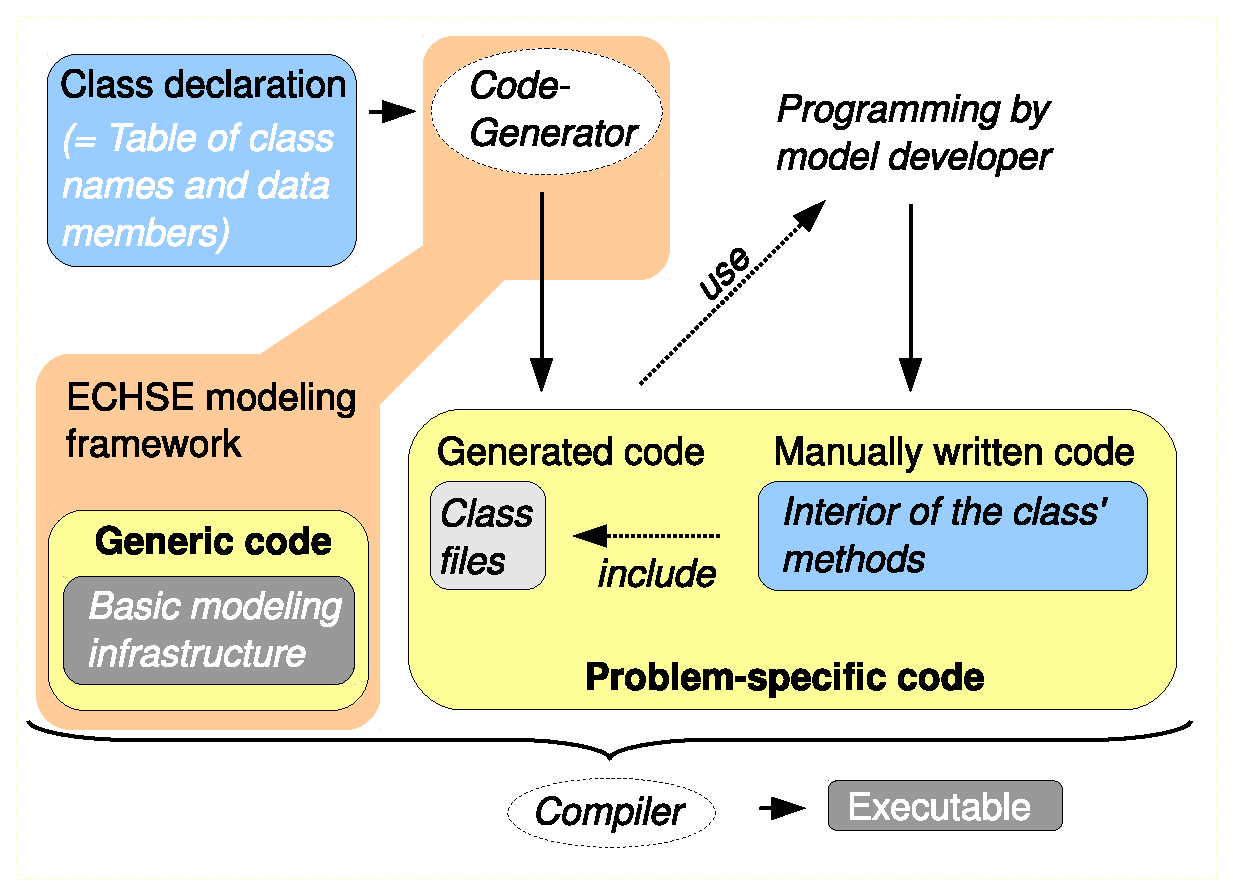
\includegraphics[width=0.9\columnwidth]{\figdir/echseIdea/echseIdea.eps}
  \caption{Major components of the \software{echse} modeling framework. \label{fig:concept-autocode-role}}
\end{figure}

To sucessfully build a simulation model with the \software{echse} framework, the problem-specific part of the source code (class definitions) must be perfectly compatible with the generic model core on the one hand. On the other hand, good practice of software development requires that the generic core and the problem specific extensions are well separated. In fact, a developer who implements the problem-specific classes should not need to understand or even know any details of the generic core.

In the \software{echse} modeling framework, this dilemma is solved by means of automatic source code generation (\figref{fig:concept-autocode-role}). In this concept, the model developer first \emph{declares} a class by specifying the names and types of all data members (see \figref{fig:concept-classFeatures-overview} for possible member types). In a second step, a program automatically generates the class' basic source code from the provided declaration. This generated code is guaranteed to be compatible with the generic core. It provides entry points for additional source code which has to be manually written in a third step. This manually written code comprises the bodies of the 'simulate' and the 'derivsScal' methods (see \secsref{sec:concept-classFeatures-simulateMethod} and \ref{sec:concept-classFeatures-derivsScal}).

The three steps of
\begin{enumerate}
  \item Declaration of data members
  \item Code generation
  \item Implementation of methods
\end{enumerate}
are illustrated in \secref{sec:concept-classDef} with the example of a linear reservoir class.

The advantages of the strategy of automatic code generation can be summarized as follows:
\begin{itemize}
  \item The model developer does not need to manually write all the abstract code related to the classes and the corresponding object groups (recall \secref{sec:concept-terms-summary}). This reduces development times for new models.
  \item The model developer does not need to care for the compatibility of the application-specific code with the code forming the generic core of any \software{echse} model. This makes model development really a simple and save task.
\end{itemize}

\subsection{The code generator} \label{sec:concept-autocode-codegen-basic}

\index{code generator}

\subsubsection*{Installation}
The code generator is currently implemented in the R programming language. It is contained in the R-package \software{codegen} which provides a single method whose name is \texttt{generate}. The package is provided as a tarball with name \verb!codegen_x.y.tar.gz! where x.y is a version number. See \citet{Echse-Install-Doc} for details on how to install the R software and add-on packages. The \software{codegen} package depends on no other packages.

\subsubsection*{Standard documentation}
After the \software{codegen} package has been loaded, for example using the R command

\begin{lstlisting}[style=R]
library("codegen")
\end{lstlisting}

the documentation of the \texttt{generate} method can be displayed by typing the question mark followed by the method's name.

\begin{lstlisting}[style=R]
?generate
\end{lstlisting}

\subsubsection*{Examples}
To run an illustrative example, one can use the following R command.

\begin{lstlisting}[style=R]
example("generate")
\end{lstlisting}

It generates sample input files for the \texttt{generate} method and then runs the method on these files. Another practical example, can be found in \secref{sec:concept-classDef}.

\subsection{Inputs of the code generator} \label{sec:concept-autocode-codegen-input}

The code generator assumes that each class is declared in a \emph{separate} file. Such a class declaration file must be a plain, TAB-separated text file with two columns 'type' and 'name' (see \figref{fig:concept-classDef-declaration-example} for an example). Each record in this table declares a single data member of the class. The meaning of the two columns is as follows:

\begin{columndef}
  \item [type] (\textit{string}) The type of the feature to be declared. Valid entries are listed in \tabref{tab:concept-featuretypes}.
  \item [name] (\textit{string}) The name of the variable, parameter, or function to be declared. The name must be a valid C++ identifier.
\end{columndef}

In addition to these two mandatory columns, the table may have additional columns which are ignored during processing by the code generator. For the purpose of documentation, it is recommended to append at least one column with a short description of each feature and probably the physical units. Moreover, the file may contain comment lines starting with the \verb!#! character (see example in \figref{fig:concept-classDef-declaration-example}). It may be  convenient to prepare the table in a spreadsheet software first and to save the contents to a text file later (by copy \& paste, for example).

\begin{table}[htb]
  \caption[Description of the keywords expected in the 'type' column of a class declaration table.]{Description of the keywords expected in the 'type' column of a class declaration table (see example in \figref{fig:concept-classDef-declaration-example}). \label{tab:concept-featuretypes}}
  \begin{tabularx}{\columnwidth}{lX} \hline\hline
    Keyword & Type of feature \\ \hline
    \texttt{stateScal} & Scalar state variable \\
    \texttt{stateVect} & Vector state variable \\
    \texttt{inputExt} & External input variable \\
    \texttt{inputSim} & Simulated input variable \\
    \texttt{paramNum} & Object-specific scalar parameter \\
    \texttt{sharedParamNum} & Group-specific scalar parameter \\
    \texttt{paramFun} & Object-specific parameter function \\
    \texttt{sharedParamFun} & Group-specific parameter function \\
    \texttt{output} & Output variable \\
    \hline\hline
  \end{tabularx}
\end{table}

\subsection{Outputs of the code generator} \label{sec:concept-autocode-codegen-output}

The code generator produces several C++ header files (file extension '.h'). The individual files are only briefly described here. The files' contents is not shown.
\begin{description}
  \item [Instantiation function definition file] This file contains a function which, when called, creates a single instance of each object group based on class template. The function returns a handle to the object groups (in the form of a pointer vector).
  \item [Header bundle file] This file contains C++ include statements, referencing all header files created by the code generator, except for the file itself. This provides a means to include a variable (application-specific) number of header files into the generic source files without the need for any modification there.
  \item [Class header file(s)] For each class declared by the model developer, a header file is generated. It describes the abstract prototype of an object of the respective class. Note that the implementation of the class' methods 'simulate' or 'derivsScal' are  \emph{not} contained here. Instead, references to include files are generated and these include files must be manually filled with code by the model developer.
  \item [Index constants file(s)] For each class declared by the model developer, a file with index constants is created. These index constants must be used when querying or manipulating an object's data via the methods described in \tabsref{tab:concept-dataAccessFunctions_read} and \ref{tab:concept-dataAccessFunctions_write}. The automatically defined constants allow for referencing a particular variable, parameter, or function \emph{by name} (see the 'name' argument in \tabref{tab:concept-dataAccessFunctions_read} and the examples in \secref{sec:concept-classDef-simulate}). This makes data access convenient, efficient, and save at the same time.
\end{description}

%%%%%%%%%%%%%%%%%%%%%%%%%%%%%%%%%%%%%%%%%%%%%%%%%%%%%%%%%%%%%%%%%%%%%%%%%%%%%%%%
%%%%%%%%%%%%%%%%%%%%%%%%%%%%%%%%%%%%%%%%%%%%%%%%%%%%%%%%%%%%%%%%%%%%%%%%%%%%%%%%
%%%%%%%%%%%%%%%%%%%%%%%%%%%%%%%%%%%%%%%%%%%%%%%%%%%%%%%%%%%%%%%%%%%%%%%%%%%%%%%%

\FloatBarrier

\section{Example: Implementing a new class} \label{sec:concept-classDef}

%%%%%%%%%%%%%%%%%%%%%%%%%%%%%%%%%%%%%%%%%%%%%%%%%%%%%%%%%%%%%%%%%%%%%%%%%%%%%%%%
\subsection{Linear reservoir} \label{sec:concept-classDef-linReserv}

In this example, we implement a class describing a so-called 'single linear reservoir'. The linear reservoir is a widely used conceptual model in the field of hydrology. Applications range from describing the storage of water in catchments to flow routing in rivers. A single linear reservoir (\figref{eqn:concept-classDef-linReserv-sketch}) is fully described by two equations: the continuity equation represenring the mass balance (\eqnref{eqn:concept-classDef-linReserv-continuity}) and the linear outflow equation (\eqnref{eqn:concept-classDef-linReserv-outflow}).

\begin{align}
  \frac{dv}{dt} = q_{in} - q_{ex} \label{eqn:concept-classDef-linReserv-continuity} \\
  q_{ex} = \frac{1}{k} \cdot v \label{eqn:concept-classDef-linReserv-outflow}
\end{align}

The symbols in the above equations are defined below where L and T are generic units of length and time, respectively.

\begin{tabular}{ll}
  $v$ &      Storage volume (L$^3$) \\
  $q_{in}$ & Rate of inflow (L$^3$/T) \\
  $q_{ex}$ & Rate of outflow (L$^3$/T) \\
  $k$ &      Retention constant (T) \\
\end{tabular}

\begin{figure}[h!bt]
  \centering
  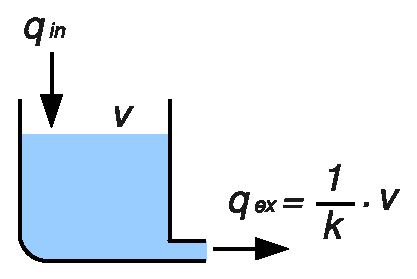
\includegraphics[width=0.4\columnwidth]{\figdir/classDef_linearReserv/linReserv.eps}
  \caption{Sketch of a single linear reservoir. \label{eqn:concept-classDef-linReserv-sketch}}
\end{figure}

The ordinary differential equation that results from combining \eqnsref{eqn:concept-classDef-linReserv-continuity} and \ref{eqn:concept-classDef-linReserv-outflow} can be solved analytically. With the simplest assumption of a constant inflow rate $q_{in}$ over a time step of length $\Delta t$ the integration yields \eqnref{eqn:concept-classDef-linReserv-solution-v}, where $v(t_0)$ is the initial storage at time $t_0$.

\begin{equation} \label{eqn:concept-classDef-linReserv-solution-v}
v(t_0 + \Delta t) = \left( v(t_0) - q_{in} \cdot k \right) \cdot e^{(-\Delta t/k)} + q_{in} \cdot k
\end{equation}

Using \eqnref{eqn:concept-classDef-linReserv-outflow} one can also transform \eqnref{eqn:concept-classDef-linReserv-solution-v} into an expression for the outflow rate $q_{ex}$ (\eqnref{eqn:concept-classDef-linReserv-solution-q}).

\begin{equation} \label{eqn:concept-classDef-linReserv-solution-q}
q_{ex}(t_0 + \Delta t) = \left( q_{ex}(t_0) - q_{in} \right) \cdot e^{(-\Delta t/k)} + q_{in}
\end{equation}

%%%%%%%%%%%%%%%%%%%%%%%%%%%%%%%%%%%%%%%%%%%%%%%%%%%%%%%%%%%%%%%%%%%%%%%%%%%%%%%%
\subsection{Step 1: Declaration of the class} \label{sec:concept-classDef-declaration}

To declare a new class, the model developer simply needs to specify the class' \emph{data members} (recall \secref{sec:concept-classFeatures-overview}). With respect to the example of the linear reservoir (\secref{sec:concept-classDef-linReserv}), one would have to declare
\begin{itemize}
  \item a single scalar state variable (storage volume $v$).
  \item a single scalar parameter (retention constant $k$). We assume here that this parameter is object-specific, \ie{} each linear reservoir has an individual $k$.
  \item a single input variable (inflow rate $q_{in}$). We assume here that this is a simulated input rather than an external input (recall \secref{sec:concept-classFeatures-inputs}).
  \item a single output variable (outflow rate $q_{ex}$)
\end{itemize}

As described in \secref{sec:concept-autocode-codegen-input}, this information has to be collected in a table-formatted text file for later processing by the code generator (\secref{sec:concept-classDef-codegen}). An appropriate input file for the code generator is shown in \figref{fig:concept-classDef-declaration-example}.

\begin{figure}[htb]
  \lstinputlisting[style=txt,linewidth=\columnwidth]{\figdir/classDef_linearReserv/declaration.txt}
  \caption[Input file for the code generator, containing the declaration of a linear reservoir class.]{Input file for the code generator, containing the declaration of a linear reservoir class. See \tabref{tab:concept-featuretypes} for the entries allowed in the 'type' column. \label{fig:concept-classDef-declaration-example}}
\end{figure}

%%%%%%%%%%%%%%%%%%%%%%%%%%%%%%%%%%%%%%%%%%%%%%%%%%%%%%%%%%%%%%%%%%%%%%%%%%%%%%%%
\subsection{Step 2: Code generation} \label{sec:concept-classDef-codegen}

Once all data members of all classes have been declared in the required form (see \secref{sec:concept-autocode-codegen-input} and \figref{fig:concept-classDef-declaration-example}), the table is further processed by the code generator\index{code generator}. Assuming that the contents of \figref{fig:concept-classDef-declaration-example} is saved in a file 'linRes.txt', an appropriate call to the code generator could be:

\begin{lstlisting}[style=R]
library("codegen")
generate(
  files=c(linReserv="linRes.txt"),
  outdir="generated_code"
  overwrite=TRUE
)
\end{lstlisting}

Note that the vector of class declaration files passed to the \texttt{files} argument must have as many elements as there are classes in the model. In our minimum example with only a single class, this vector is of lenght 1. Also note that this must be a \emph{named} vector because the class' names are generated from the elements' names. Thus, the name for the linear reservoir class would be 'linReserv' in the above example.

The complete output from the above call to the \texttt{generate} method is not presented here. An an overview of the created files was already given in \secref{sec:concept-autocode-codegen-output} and a central part of the generated code is shown in \figref{fig:concept-classDef-methodsFrame}.

%%%%%%%%%%%%%%%%%%%%%%%%%%%%%%%%%%%%%%%%%%%%%%%%%%%%%%%%%%%%%%%%%%%%%%%%%%%%%%%%
\subsection{Step 3: Implementing the class' methods} \label{sec:concept-classDef-simulate}

As mentioned in \secsref{sec:concept-autocode-role} and \ref{sec:concept-autocode-codegen-output}, the implementation (\ie{} the body code) of the 'simulate' and 'derivsScal' methods has to be provided by the model developer. The code generator only creates appropriate method interfaces and include statements. For the linear reservoir class introduced in \secref{sec:concept-classDef-linReserv}, part of the generated code is shown in \figref{fig:concept-classDef-methodsFrame}.

\begin{figure*}
  \lstinputlisting[style=c++, framexleftmargin=0mm, numbers=left, stepnumber=1, numbersep=2mm, numberstyle=\ttfamily\footnotesize, firstline={40}] {\figdir/classDef_linearReserv/AUTOechse_userClass_linReserv.h}
  \caption{Part of the generated header file for the linear reservoir class showing the frame of the 'simulate' and 'derivsScal' methods. The manually written code is imported by the \texttt{\#include} directives. \label{fig:concept-classDef-methodsFrame}}
\end{figure*}

Two complete, alternative bodys of the 'simulate' and 'derivsScal' methods of the linear reservoir class are presented in  \figref{fig:concept-classDef-implementation-analytical} \& \ref{fig:concept-classDef-implementation-numerical}. This is the code which would be imported by the \verb!#include! directives in \figref{fig:concept-classDef-methodsFrame}.

\begin{figure*}
  File '\verb!userCode_linReserv_aux.cpp!'
  \lstinputlisting[style=c++, framexleftmargin=0mm, numbers=left, stepnumber=1, numbersep=2mm, numberstyle=\ttfamily\footnotesize]{\figdir/classDef_linearReserv/userCode_linReserv_analytical-aux.cpp}
  File '\verb!userCode_linReserv_simulate.cpp!'
  \lstinputlisting[style=c++, framexleftmargin=0mm, numbers=left, stepnumber=1, numbersep=2mm, numberstyle=\ttfamily\footnotesize]{\figdir/classDef_linearReserv/userCode_linReserv_analytical-simulate.cpp}
  File '\verb!userCode_linReserv_derivsScal.cpp!'
  \lstinputlisting[style=c++, framexleftmargin=0mm, numbers=left, stepnumber=1, numbersep=2mm, numberstyle=\ttfamily\footnotesize]{\figdir/classDef_linearReserv/userCode_linReserv_analytical-derivsScal.cpp}
  \caption[Bodies of the 'simulate' and 'derivsScal' methods for the linear reservoir class if an analytical solution is adopted.]{Bodies of the 'simulate' and 'derivsScal' methods for the linear reservoir class if an analytical solution is adopted. \label{fig:concept-classDef-implementation-analytical}}
\end{figure*}

\begin{figure*}
  File '\verb!userCode_linReserv_aux.cpp!'
  \lstinputlisting[style=c++, framexleftmargin=0mm, numbers=left, stepnumber=1, numbersep=2mm, numberstyle=\ttfamily\footnotesize]{\figdir/classDef_linearReserv/userCode_linReserv_numerical-aux.cpp}
  File '\verb!userCode_linReserv_simulate.cpp!'
  \lstinputlisting[style=c++, framexleftmargin=0mm, numbers=left, stepnumber=1, numbersep=2mm, numberstyle=\ttfamily\footnotesize]{\figdir/classDef_linearReserv/userCode_linReserv_numerical-simulate.cpp}
  File '\verb!userCode_linReserv_derivsScal.cpp!'
  \lstinputlisting[style=c++, framexleftmargin=0mm, numbers=left, stepnumber=1, numbersep=2mm, numberstyle=\ttfamily\footnotesize]{\figdir/classDef_linearReserv/userCode_linReserv_numerical-derivsScal.cpp}
  \caption[Bodies of the 'simulate' and 'derivsScal' methods for the linear reservoir class if a numerical solution is adopted.]{Bodies of the 'simulate' and 'derivsScal' methods for the linear reservoir class if a numerical solution is adopted. Note that the value of the volume state variable ($v$) in the 'derivsScal'method is accessed via \texttt{u[INDEX\_v]} instead of \texttt{stateScal(v)}. \label{fig:concept-classDef-implementation-numerical}}
\end{figure*}

%%%%%%%%%%%%%%%%%%%%%%%%%%%%%%%%%%%%%%%%%%%%%%%%%%%%%%%%%%%%%%%%%%%%%%%%%%%%%%%%
\subsection{Step 4: Compilation} \label{sec:concept-classDef-compile}

Once the code generator has run successfully and the methods for all classes are implemented, the application specific simulation software (\ie{} the 'model engine') has to be build. This is achieved by compiling and linking all parts of the source code, namely
\begin{enumerate}
  \item the static part of the code, providing the basic infrastructure for every model.
  \item the application-specific code created by the code generator (see \secref{sec:concept-classDef-codegen}).
  \item the body code of the 'simulate' and 'derivsScal' methods, manually written by the model developer.
\end{enumerate}

The GNU C++ compiler is used for this purpose and the procedure has been successfully tested on several platforms. To assist the developer in the compilation process, platform-specific makefiles are available.

If invalid code is detected in the manually written parts of the code, the compilation will fail, of course and one has to go through the usual steps of debugging. One should keep in mind, however, that a successful compilation does not necessarily mean that the code is 'correct' in the sense that it produces the desired results. The correctness of the code can only be verified by analyzing the model's output.

%%%%%%%%%%%%%%%%%%%%%%%%%%%%%%%%%%%%%%%%%%%%%%%%%%%%%%%%%%%%%%%%%%%%%%%%%%%%%%%%
%%%%%%%%%%%%%%%%%%%%%%%%%%%%%%%%%%%%%%%%%%%%%%%%%%%%%%%%%%%%%%%%%%%%%%%%%%%%%%%%
%%%%%%%%%%%%%%%%%%%%%%%%%%%%%%%%%%%%%%%%%%%%%%%%%%%%%%%%%%%%%%%%%%%%%%%%%%%%%%%%

\FloatBarrier

\section{Outline of computational steps} \label{sec:concept-compSteps}

\subsection{Overview} \label{sec:concept-compSteps-overview}

The essential computational steps carried out when executing a model are summarized in \figref{fig:concept-compSteps}. Note that this outline applies to \emph{any} model built with the \software{echse} simulation environment.

\begin{figure}[h]
\smallskip
\textit{Main function} \\
\colorbox{shadecolor}{
\begin{minipage}{0.95\columnwidth}
  \smallskip
  \begin{itemize}
    \item Retrieval of command line arguments (\secref{sec:input-commandline})
    \item Reading of the configuration file (\secref{sec:input-config})
    \item Instantiation of objects \& object groups (see \figref{fig:concept-terms_implementation})
    \item Initialization of the objects' data.
  \end{itemize}
  \smallskip
    \textit{Loop over time steps} \\
    \framebox{
    \begin{minipage}{0.9\columnwidth}
      \smallskip
      \begin{itemize}
         \item Updating of external inputs
      \end{itemize}
      \smallskip
      \textit{Loop over objects} \\
      \framebox{
      \begin{minipage}{0.85\columnwidth}
        \smallskip
        \begin{itemize}
           \item Call of the 'simulate' method for current object
        \end{itemize}
      \end{minipage}
      }
      \begin{itemize}
         \item Writing of data to output files
      \end{itemize}
    \end{minipage}
    }
    \begin{itemize}
      \item Closing of output files
    \end{itemize}
  \begin{itemize}
    \item Clean-up
    \item Output of traceback info in case of exceptions
    \item Setting of return code and termination
  \end{itemize}
\end{minipage}
}
  \caption[Essential computational steps of a model run.]{Essential computational steps of a model run. The framed boxes represent loops, thus the tasks inside these boxes are executed repeatedly (see \secref{sec:concept-compSteps-loopNesting}). \label{fig:concept-compSteps}}
\end{figure}

Most of the computational steps listed in \figref{fig:concept-compSteps} appear in any dynamic systems simulation software. Only those aspects which are specific to \software{echse} models are discussed in the subsequent sections.

\subsection{Time and object loop} \label{sec:concept-compSteps-loopNesting}

In \figref{fig:concept-compSteps}, the innermost framed box represents the so-called \emph{object loop}. The purpose of this loop to iterate through all objects and trigger the simulation for a single time step by calling the objects' 'simulate' methods (see \secref{sec:concept-classFeatures-simulateMethod}). In a spatially distributed model, the term 'spatial loop' is often an appropriate synonym for 'object loop'\footnote{In the current version of the software, the object loop is split into two nested loops to enable parallel processing. This is not essential for the understanding for the general understanding, however.}.

Note that the \emph{time loop} is wrapped around the object loop (\figref{fig:concept-compSteps}). This design can be found in virtually all spatially distributed models that solve \emph{partial} differential equations (PDE) such as groundwater flow models or hydrodynamic models. Note, however, that a few models exist where the two loops are in reverse order, for example in some hydrological catchment models.

The consequence of having the object loop \emph{inside} the time loop is that, for a particular time step, the 'simulate' method is executed for \emph{all} objects, before the computation proceeds with the subsequent time step. This allows for the exchange of information between objects in every single time step. This is a precondition for properly handling \emph{feedbacks} between objects, \ie{} two-way interactions (see \figref{fig:concept-interactions-types}, \secref{sec:concept-interactions-types}).

The only drawback of this approach is the requirement of keeping instances of \emph{all} objects in memory at the same time. Thanks to the large memory capacity of modern computers, this is hardly an issue. If the number of objects should actually be too large to fit into memory, a cheap solution would be to split the model (into spatial sub-domains, for example) in a way that no feedback between the sub-models does occur.

\subsection{Exception handling} \label{sec:concept-compSteps-exceptionHandling}

In a complex and flexible software it is not unlikely that an unrecoverable error occurs during computations. The potential causes are manifold, ranging from missing or erroneous input data to mathematical calculations yielding invalid results (NaN, Inf, ect.).

The models built with the \software{echse} simulation environment use C++'s exceptions\index{exceptions} mechanism to handle situations like that. Whenever an exception occurs, the normal execution of the program is suspended and priority is given to exception handling. In the case of \software{echse} models, this means that the currently active unit (\ie{} a class method or function) tries to collect as many information as possible about the circumstances of the exception and then gives control back to its calling unit. The calling unit behaves just like the unit where the exception originally occurred. In this way, the error signal is passed through the hierarchy of routines and finally causes an exception at the highest level, the 'main' function. Here (and only here), traceback\index{traceback} information is generated and the program is forced to terminate (see final step in \figref{fig:concept-compSteps}).

The traceback always contains (for every unit) information about
\begin{enumerate}
  \item the name of the unit, where the exception occurred.
  \item a description of the circumstances and possibly the cause of the exception.
  \item the name of the source file containing the unit that failed.
  \item the line of this file where the exception was thrown.
\end{enumerate}

Based on the traceback information, the location and cause of the error can usually be  identified with little effort.

If the model terminated due to an exception, the program issues a non-zero return code. If no exception occurred, a the code of zero is returned as this is widely used convention. The return code should always be checked if the model is embedded in another software such as a scripts or batch files.

%%%%%%%%%%%%%%%%%%%%%%%%%%%%%%%%%%%%%%%%%%%%%%%%%%%%%%%%%%%%%%%%%%%%%%%%%%%%%%%%
%%%%%%%%%%%%%%%%%%%%%%%%%%%%%%%%%%%%%%%%%%%%%%%%%%%%%%%%%%%%%%%%%%%%%%%%%%%%%%%%
%%%%%%%%%%%%%%%%%%%%%%%%%%%%%%%%%%%%%%%%%%%%%%%%%%%%%%%%%%%%%%%%%%%%%%%%%%%%%%%%

\section{Interactions between objects} \label{sec:concept-interactions}


\subsection{Overview and accessible data} \label{sec:concept-interactions-access}

Interactions \index{object!interaction}\index{interactions|see{object interaction}} between objects are a typical in natural and technical systems. In this context, an interaction is defined as an exchange of either matter (mass), energy, or information. Although it is possible to simulate just a single object or a group of non-interacting objects, interactions have to be considered in the vast majority of real-world models.

As already outlined in \secsref{sec:concept-classFeatures-inputs} and \ref{sec:concept-classFeatures-outputs}, an interaction between two objects is bound to the declaration of
\begin{enumerate}
  \item a \emph{simulated input variable} in the class corresponding to the object that \emph{uses} data provided by another object.
  \item an \emph{output variable} in the class corresponding to the object that \emph{provides} the data to be used by (an)other object(s).
\end{enumerate}

In a dynamic simulation model with sequential processing of the objects (see \secref{sec:concept-compSteps-loopNesting} and \figref{fig:concept-compSteps}), further limitations with respect to the acessibility of data do exist. This is illustrated in \figref{fig:concept-interactions-access} from the perspective of a single object with respect to a single time step (bold-framed object $M_k$). Assuming that appropriate simulated input and output variables have been declared in the respective classes (see above), for the simulation of time step $i$, the object $M_k$ has access to
\begin{enumerate}
  \item data on the object itself, representing the state at the end of the previous time step with index $i-1$.
  \item the output variables of the already processed \emph{upstream} objects. These values are representative for the end of the \emph{current} time step ($i$).
  \item the output variables of the \emph{downstream} objects still waiting for being simulated. These values are representative for the end of the \emph{previous} time step ($i-1$).
\end{enumerate}

\begin{figure}
  \centering
  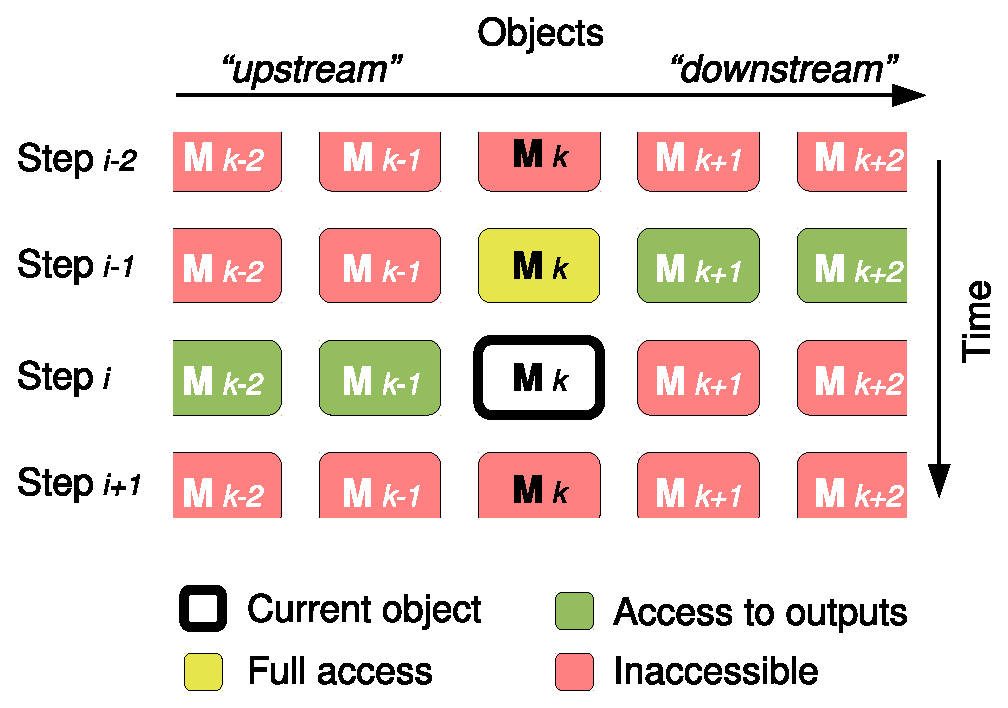
\includegraphics[width=0.9\columnwidth]{\figdir/interactions/interactions_access.eps}
  \caption{Accessible data from a single object's perspective. \label{fig:concept-interactions-access}}
\end{figure}

\subsection{Types of interactions} \label{sec:concept-interactions-types}

Looking at two interacting objects, one generally has to distinguish between \emph{feed-forward} interactions (also called \emph{one-way} interactions) and \emph{feedbacks}, also known as \emph{two-way} interactions (\figref{fig:concept-interactions-types}). The difference between the two is illustrated also in \figref{fig:concept-interactions-bucketExample} on a very simple example. Typical real-world examples of feedbacks in the field of hydrology include
\begin{itemize}
  \item interactions between river and floodplain. River stage and groundwater level are coupled via inflitration and leakage, respectively.
  \item diffusion problems at the interface of the pelagic and benthic zone. The rate of diffusive transport depends on both, the concentration in the water body and the sediment's pore water.
  \item the operational control of a reservoir's outflow based on stream flow data observed at a gage downstream of the reservoir.
\end{itemize}

\begin{figure}
  \centering
  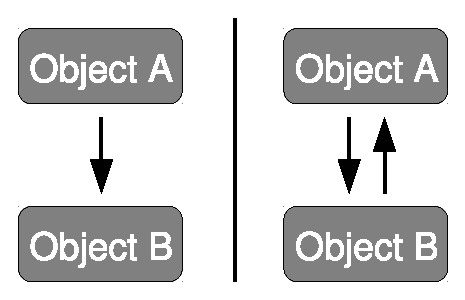
\includegraphics[width=0.5\columnwidth]{\figdir/interactions/interactions_types.eps}
  \caption[Basic types of object interaction.]{Basic types of object interaction. The arrows indicate exchange of matter, energy, or information. Left: Feed-forward type. Right: Feedback type. \label{fig:concept-interactions-types}}
\end{figure}

\begin{figure}
  \centering
  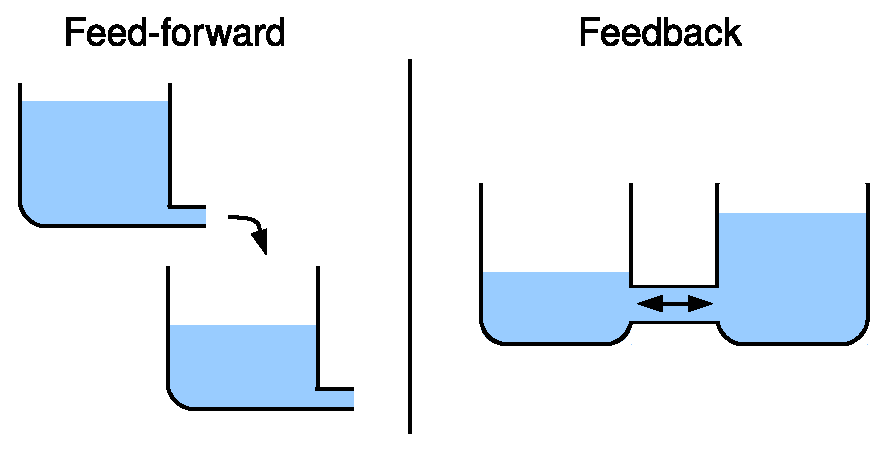
\includegraphics[width=0.75\columnwidth]{\figdir/interactions/interactions_buckets.eps}
  \caption{Types of interactions between two buckets filled with a liquid. \label{fig:concept-interactions-bucketExample}}
\end{figure}

The feedback (\figsref{fig:concept-interactions-types} \& \ref{fig:concept-interactions-bucketExample}, right) represents the more general type of interaction and, actually, the feed-forward interaction (\figsref{fig:concept-interactions-types} and \ref{fig:concept-interactions-bucketExample}, left) may be regarded just as a special type of (missing) feedback. It makes sense, however, to strictly distinguish between the two types of interaction in the context of dynamic simulation, \ie{} when modeling the interaction of objects over a sequence of discrete time steps. This is due to the following:

\begin{description}
  \item [Feed-forward type] As long as the exchange of data between two interacting objects 'A' and 'B' is effectively \emph{one-way}, the two objects can be simulated \emph{sequentially}, \ie{} one after another. The so-called \emph{source object} ('A' in \figref{fig:concept-interactions-types}, left) represents the 'data provider' and must be simulated first. The output of 'A' is then used as an input for the \emph{target object} ('B'), which is simulated later.
  \item [Feedback type] If there is a \emph{two-way} exchange of data between two objects 'A' and 'B', these objects must be simulated \emph{simultaneously}, \ie{} at the same time. To put it in other words: The ordinary differential equations, describing the evolution of the state variables in object 'A' form a coupled system with the equations of object 'B'. To get a proper solution, the coupled differential equations must be integrated simultaneously using an ODE solver \citep[see \eg{}][]{Press2002}. This, however, conflicts with the facts that (1) objects are geberally treated as well-separated entities and (2) the array of objects is processed sequentially using a fixed order (see innermost loop in \figref{fig:concept-compSteps}). Nevertheless, \software{echse}-based models are capable of handling feedback interactions using the techniques outlined in \secref{sec:concept-interactions-feedbackHandling}.
\end{description}

\subsection{Handling of feedbacks} \label{sec:concept-interactions-feedbackHandling}

\subsubsection*{Option 1: Compound classes}

A straightforward approach to cope with the problem of feedback interactions (\secref{sec:concept-interactions-types}) is to avoid inter-object feedbacks. Taking the objects 'A' and 'B' from \figref{fig:concept-interactions-types} (right) as an example, this would mean that the class(es), of which the objects 'A' and 'B' are instances, are joined to form a new (compound) class. The feedback interaction between the former objects 'A' and 'B' is then \emph{internally} present in an object of the compound class. The coupled differential equations related to all state variables (which were originally distributed over object 'A' and 'B') can then be solved simultaneously using a standard ODE solver within the simulate method (\secref{sec:concept-classFeatures-simulateMethod}) of the compound class.

The drawback of such an approach is that the compound class may quickly become rather complex. In extreme cases of many feedback interactions, one might end up with a model consisting of only a single object being an instance of a single class which basically integrates 'everything'. In such a case one should think about other strategies (see below) or use another, more appropriate modeling software.

\subsubsection*{Option 2: Step-wise feedback}

The simplest and probably the most common solution for the feedback problem is to treat the differential equations in the two interacting objects 'A' and 'B' as \emph{temporarily independent}. In practice, this works as follows:
\begin{description}
  \item [Simulation step] The objects 'A' and 'B' are simulated independendly, as if there was no interaction at all. This means that the state variables of 'A' and 'B' are updated by separately integrating the respective differential equations.
  \item [Feedback step] After \emph{every} time step, the two objects exchange information about their new states. The information about 'A' is then used in the subsequent simulation step for 'B' and vice versa.
\end{description}

To make the described approach of \emph{step-wise feedback} successfully work in practice, two conditions must be met.

Firstly, the interacting objects 'A' and 'B' must exchange data with a high frequency. This is achieved by running the simulation in small time steps. The longer the time step, the higher the potential numerical error will be.

Secondly, it has to be ensured that the information about object 'B' used by 'A' refers to the \emph{same point in time} as the information about 'A' used by 'B'. In a normal sequential simulation, where either 'A' or 'B' is processed first, this is not the case. However, with the help of a so-called \emph{observer object} it is possible to supply 'A' and 'B' with data of equal up-to-dateness, in spite of sequential processing. This strategy is illustrated by \figref{fig:concept-interactions-observer}. In the shown example, a feedback interactions exists between the objects $M_k$ and $M_{k+1}$. The role of the auxiliary observer object $M_{k-1}$ is to collect data on $M_k$ and $M_{k+1}$ which is representative for a particular point in time, namely the (end of) time step $i-1$. The collected information is then supplied to $M_k$ and $M_{k+1}$, respectively, to be used in the simulation over the current time step $i$.

\begin{figure}
  \centering
  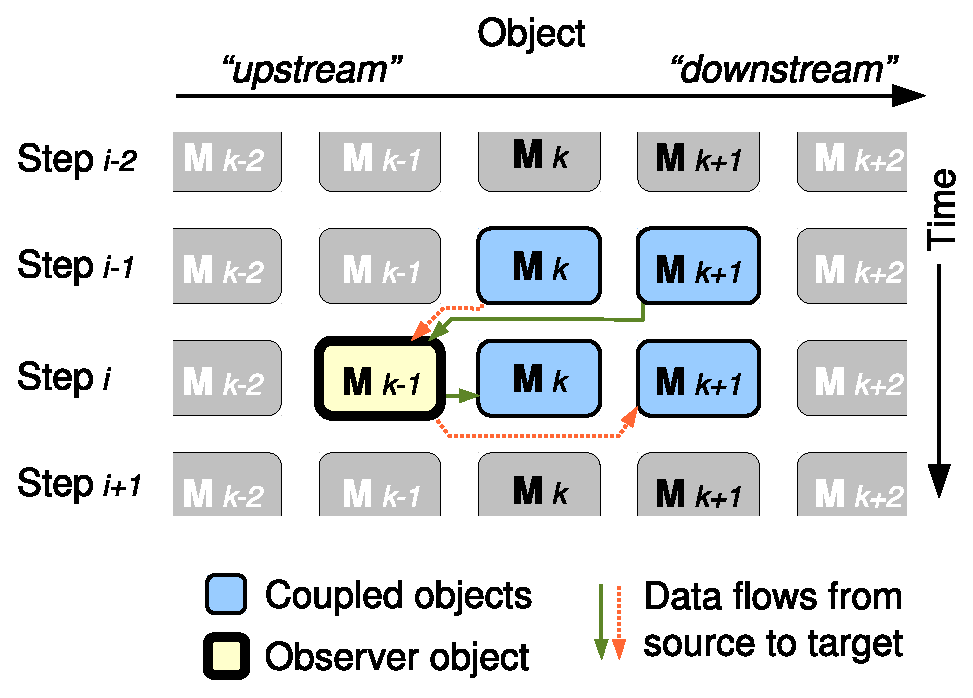
\includegraphics[width=0.9\columnwidth]{\figdir/interactions/interactions_observer.eps}
  \caption{Use of an artificial \emph{observer object} to provide two sequentially processed, feedback-coupled objects with information of equal up-to-dateness. \label{fig:concept-interactions-observer}}
\end{figure}

\subsubsection*{Step-wise feedback: Time step issues}

As mentioned above, the selection of a sufficiently short time steps is necessary to keep the error associated with the step-wise handling of feedbacks within acceptable limits. A disadvantage of the current version of the \software{echse} is that the time step is a fixed parameter. Consequently, if a short time step is selected with the intention of increasing the accuracy of feedback solutions, the computation will slow down even for those objects which are not subject to feedback interactions. Thus, a single feedback interaction may impact negatively on the performance of the entire model in terms of computation time. A possible solution to this problem lies in releasing the constraints of the fixed 'global' time step. In particular, it would make sense allow a variable number of sub-steps to be specified for each object. The only restriction would be that the number of sub-steps must be identical for two objects having a feedback relation. If a feedback interaction exists between two objects 'A' and 'B' and another one exists between two objects 'C' and 'D', the number sub-steps applied to the first group ('A', 'B') and the second group ('C', 'D') may still be different, however. It is planned to implement the sub-step approach in an upcoming version of the \software{echse}.

\subsubsection*{Step-wise feedback: Accuracy}

To really understand the limits of the strategy of a step-wise simulation of feedbacks, a closer look on the solution strategy is required. Let's take the example of \figref{fig:concept-interactions-observer}, where a feedback interaction between the objects $M_k$ and $M_{k+1}$ is simulated under the control of an observer object $M_{k-1}$. In a first step, the observer object $M_{k-1}$ collects information from both object $M_k$ and $M_{k+1}$ which is representative for time step $i-1$. If the objects $M_k$ and $M_{k+1}$ were the two connected buckets shown in the right column of \figref{fig:concept-interactions-bucketExample}, the observer $M_{k-1}$ would collect information on the water levels in the two buckets and compute the resulting flow rate. Then, the two objects $M_k$ and $M_{k+1}$ would retrieve the computed flow rate from the observer and both objects would use this information to calculate their individual water levels at the end of time step $i$.

It is important to realize that the accuracy of the resulting solution is limited by the fact that the information on the flow rate between the two buckets is a contant. This rate effectively represents the sitution at the end of time step $i-1$ or (in other words) the situation at the \emph{very beginning} of time step $i$. This \emph{constant} information is then used in the simulation of the \emph{entire} time step $i$, neglecting that the water levels change, hereby affecting the flow rate.

Solutions with these characteristics are also called \emph{Euler solutions}. It is well known that the accuracy of such first-order solutions is quite limited. Therefore, with the current version of the \software{echse} a reasonable simulation of feedbacks can only be expected if
\begin{itemize}
  \item non-linearities are weak.
  \item the chosen simulation time step is sufficiently short.
\end{itemize}

A straighforward method to examine the accuracy of the simulation of feedback interactions is to simply run the model with different time steps and to compare the results for the affected objects. It is possible that support for higher-order solutions (Heun, Runge-Kutta, etc.) and/or methods of automatic time step control will be implemented in a future version of the \software{echse}.

\subsection{Conservation of mass or energy}

As explained earlier, information is not continuously exchanged between interacting objects but only after discrete time steps. This is true for both feed-forward and feedback interactions. In the usual case of non-linear dynamics, it is quite important to understand the consequences with respect to the loss of accuracy and regarding the conservation of mass or energy in particular.

Recall the example of the two separate buckets shown at the left side of \figref{fig:concept-interactions-bucketExample}. In this feed-forward interaction, the bucket at the bottom receives inflow from the other bucket. If we assume that the upper bucket has the characteristics of a linear reservoir (see \secref{sec:concept-classDef-linReserv}) we known from \eqnref{eqn:concept-classDef-linReserv-solution-q} (page \pageref{eqn:concept-classDef-linReserv-solution-q}) that the outflow is a \emph{non-linear} (exponential) function of time (\figref{fig:concept-interactions-accuracy}).

\begin{figure}
  \centering
  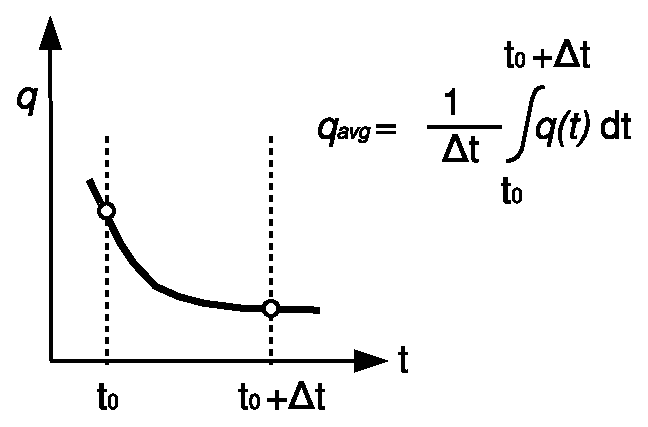
\includegraphics[width=0.6\columnwidth]{\figdir/interactions/interactions_accuracy.eps}
  \caption{Example outflow $q$ from a linear reservoir within a discrete modeling time step of length $\Delta t$. \label{fig:concept-interactions-accuracy}}
\end{figure}

Recalling \secref{sec:concept-classFeatures-outputs}, we know that all information about the upstream bucket's outflow needs to be passed to the downstream bucket through output variables. Often, the crux for the model developer is to define the output variables in way that
\begin{enumerate}
  \item the information on the dynamics is retained.
  \item mass (or energy) is conserved.
\end{enumerate}

Unfortunately, these two goals cannot be achieved at the same time and one needs to set a priority. Based on the example from \figref{fig:concept-interactions-accuracy}, some possible options are discussed in the following.

\subsubsection*{Boundary values}

A simple solution would be to pass the values at time step boundaries through two output variables:
\begin{itemize}
  \item The flow rate at the beginning of the time step $q(t_0)$.
  \item The flow rate at the end of the time step $q(t_0 + \Delta t)$.
\end{itemize}

In this way, at least the information on the change of the flow rate within the time step is retained. However, the information on the actual non-linearity is lost. Consequently, the information on the true cumulated outflow, \ie{} the exchanged volume, is lost too.

\subsubsection*{'Improper' average}

Another option would be to pass only an average outflow rate computed as the arithmetic mean of $q(t_0)$ and $q(t_0 + \Delta t)$. In most cases, this is not recommended, because neither of the two above-mentioned goals is met. Firsty, the information on the dynamics is completely lost. Secondly, use of the average value as defined above results in a mass balance error if the true dynamics is \emph{non-linear}. This is true in the example (\figref{fig:concept-interactions-accuracy}) as well as in most real-world situations.

\subsubsection*{Intermediate values}

With this strategy, information on the outflow at intermediate times is passed. For example, one could pass the 3 values $q(t_0)$, $q(t_0 + 1/2 \Delta t)$, $q(t_0 + \Delta t)$. Then, the downstream bucket could try to re-construct the non-linear dynamics, for examply by fitting an interpolation function $g(t)$ to the three values.

\subsubsection*{Interpolation parameters}

This is just a special case of the afore-mentioned option. In this case, one does not pass the outflow rates at intermediate times. Instead, the parameters of the interpolation function $g(t)$ are passed. Depending on the specific case and the type of the interpolation function, this may reduce the number of necessary output variables.

\subsubsection*{'Proper' time-step average}

If the priority is on conservation of mass, one needs to pass a \emph{proper} average outflow rate $\overline{q_{out}}$ from the upstream to the downstream bucket. The two above-mentioned approaches allow for the calculation of an approximate average outflow rate as

\begin{equation*}
  \overline{q_{out}} \approx \frac{1}{\Delta t}\int_{t_0}^{t_0+\Delta t}g(t)
\end{equation*}

with $g(t)$ being the interpolation function. To make this work in practice, the interpolation function $g(t)$ must be integratable and allow for a reasonable fit of the dynamics.

Another strategy which is often more straightforward is based on a discrete mass balance for the upstream bucket. Denoting the volume of the upstream bucket as $v$ and assuming a \emph{constant} inflow rate $q_{in}$, the time-step averaged outflow rate $\overline{q_{out}}$ is

\begin{equation*}
  \overline{q_{out}} = q_{in} - \frac{v(t_0 + \Delta t) - v(t_0)}{\Delta t}
\end{equation*}

The approach remains applicable even if more input or loss terms appear in the bucket's mass balance. It is not even necessary that these terms are constant over the time step of length $\Delta t$, but then, their cumulated values (integrals over $\Delta t$) must be known. In practice, these integral values can be obtained by introducing auxiliary state variables representing the cumulated inputs and/or losses. These auxiliary state variables can be initialized with zero at the begin of each time step.

\subsubsection*{Combined approaches}

In some cases, it may be favourable to combine some of the approaches discussed above. For example, one could pass the values at the time-step boundaries as well as the proper time-step average value. In this way, the loss of information at the interface between the interacting objects is minimized.

\chapter{Input of \software{echse}-based models} \label{chap:input}
\renewcommand{\tabdir}{chapters/input/tab}
\renewcommand{\figdir}{chapters/input/fig}

%%%%%%%%%%%%%%%%%%%%%%%%%%%%%%%%%%%%%%%%%%%%%%%%%%%%%%%%%%%%%%%%%%%%%%%%%%%%%%%%
%%%%%%%%%%%%%%%%%%%%%%%%%%%%%%%%%%%%%%%%%%%%%%%%%%%%%%%%%%%%%%%%%%%%%%%%%%%%%%%%
%%%%%%%%%%%%%%%%%%%%%%%%%%%%%%%%%%%%%%%%%%%%%%%%%%%%%%%%%%%%%%%%%%%%%%%%%%%%%%%%
\section{Mandatory command line arguments} \label{sec:input-commandline}

Some basic settings are passed to the model via the command line\index{command line}. Each of these settings is identified by a unique keyword. The keyword must be followed by the equal sign '=', followed by a corresponding value. There must be no spaces before or after the equal sign. The expected keyword-value pairs are summarized in \tabref{tab:input-commandline}. They may appear at the command line in any order. In addition to these mandatory arguments, further configuration data may be passed via the command line (see \secref{sec:input-config}).

\begin{table*}
  \caption{Mandatory command line arguments of a model. \label{tab:input-commandline}}
  \begin{tabular}{p{0.17\textwidth}p{0.1\textwidth}p{0.63\textwidth}} \hline
    \textbf{Keyword} & \textbf{Data type} & \textbf{Description} \\ \hline
    \verb!file_control! & string &
      Name/path of the configuration file. This file contains all configuration data (except for those data specified as additional command line arguments). The configuration data are discussed in detail in \secref{sec:input-config}. \\
    \verb!file_log! & string &
      Name/path of the log file created during a model run. The log file contains a compact documentation of all major steps of processing. Its contents is usually inspected in the case of abnormal program termination. \\
    \verb!file_err! & string &
      Name/path of a file where traceback information should be written to. This file will only be generated if the model terminates after occurrence of an exception. In the vast majority of cases, the information found in this file will help to quickly identify what caused the exception. \\
    \verb!format_err! & string &
      This option controls the format used in the file specified as \verb!file_err!.  The supported codes currently include 'xml', 'html', and 'txt'. For visual inspection, the html-format is the preferred choice. The other formats are more useful for automatic extraction of information (if the model is running in a more complex software environment, for example). If an unsupported format code is supplied, the 'txt' format will be used. \\
    \verb!silent! & logical &
      The model sends basic messages about the current state of processing to standard output (usually the screen) if \verb!silent=false!. This kind of output may be suppressed by setting \verb!silent=true!.\\
    \hline
  \end{tabular}
\end{table*}

A typical call of the model in a shell script using only the mandatory arguments might look as follows:

\texttt{model \textbf{file\_control}=config.txt \textbf{file\_log}=log.txt \textbf{file\_err}=err.html \textbf{format\_err}=html \textbf{silent}=false}

%%%%%%%%%%%%%%%%%%%%%%%%%%%%%%%%%%%%%%%%%%%%%%%%%%%%%%%%%%%%%%%%%%%%%%%%%%%%%%%%
%%%%%%%%%%%%%%%%%%%%%%%%%%%%%%%%%%%%%%%%%%%%%%%%%%%%%%%%%%%%%%%%%%%%%%%%%%%%%%%%
%%%%%%%%%%%%%%%%%%%%%%%%%%%%%%%%%%%%%%%%%%%%%%%%%%%%%%%%%%%%%%%%%%%%%%%%%%%%%%%%
\section{General notes on file formats} \label{sec:input-formats}

All input files comply with a simple quasi-standard\index{format!files} and can easily be created automatically (by scripts or any spreadsheet software). For small projects, the files can even be created manually using just a text editor. The general rules applying to all input files are as follows:
\begin{description}
  \item [Tabular format] All input files actually represent tables. The number of columns varies from file to file and the number of rows (records) depends generally on the particular application. The number of columns must be consistent for all records. The tables are in plain text format.
  \item [Column separator] The table columns are separated by a reserved character which has to be specified in the configuration file (see \secref{sec:input-config}). Recommended choices are the TAB-character (ASCII code 9), and/or the blank character, or the semi-colon (quasi-standards). As an exception to the above, the column separator used in the configuration file is the equal sign ('=') and it cannot be altered by the user.
  \item [Table header] The first non-blank, non-comment line of a file is interpreted as the table header contaning column names. Tables without header are not supported.
  \item [Character set] An input file should contain nothing but ASCII characters. Other characters may or may not be interpreted correctly (to be tested).
  \item [Comment lines] Comment character(s) have to be be specified in the configuration file (see \secref{sec:input-config}). A line starting with one of the selected comment characters is ignored when reading the table.
  \item [Blank lines] Blank lines are ignored when reading the table, just like comment lines.
  \item [Platform independency] Line endings may be system specific. On Linux/unix, the standard is \verb!\n!. On Windows, it is \verb!\r\n!. Input files prepared for Linux usually also work on Windows and vice-versa (to be tested). The line endings in the output files depend on the platform on which the model is running (see standards above).
  \item [Order of columns] With one exception, the columns of a table can be in any order (since they are identified by the columns' names). The only exception are time series data files (see \secref{sec:input-timeseries}), where the time information must be in the first column. Subsequent columns (containing data values for different locations or variables) may be in any order.
  \item [Column types] The supported data types of a column are: string, integer, numeric, logical, and datetime. For numerical values the usual f-format (0.1) or the scientific e-format (1.e-01) may be used. Valid logical values are \true{} and \false{} (not case-sensitive). Datetime values must be strings in ISO 8601 format\index{format!datetime}, i.e.{} in format \texttt{YYYY-MM-DD hh:mm:ss}. Date and time must be separated by a single character (recommended is a blank).
  \item [File names] Some tables contain references to other files. A file name can be specified using either the absolute or relative path.
  \item [Empty tables] There are no optional input files, which means that all files must exist and must be readable, even if they are not required for a particular application. Even if there is no information to be filled in, you cannot just supply an empty file. Instead you must supply a proper table with the usual header line and (at least) one record of values. The values may (and should be) dummy values that are easily identified as dummies. This procedure may seem overly complicated at first but, in fact, it avoids many other problems (tests in the source code, documentation of optional files, etc.).
\end{description}

%%%%%%%%%%%%%%%%%%%%%%%%%%%%%%%%%%%%%%%%%%%%%%%%%%%%%%%%%%%%%%%%%%%%%%%%%%%%%%%%
%%%%%%%%%%%%%%%%%%%%%%%%%%%%%%%%%%%%%%%%%%%%%%%%%%%%%%%%%%%%%%%%%%%%%%%%%%%%%%%%
%%%%%%%%%%%%%%%%%%%%%%%%%%%%%%%%%%%%%%%%%%%%%%%%%%%%%%%%%%%%%%%%%%%%%%%%%%%%%%%%
\section{Units of variables and constants} \label{sec:input-units}

There is no general convention, \ie{} arbitrary units\index{units} may be used for all constants and variables. The only important facts are:
\begin{itemize}
  \item The units of all variables and constants used in any equations must be consistent. There are no (and cannot be) any built-in checks in the generic part of the source code.
  \item The length of a modeling time step passed to the classes' simulate methods as argument \verb!delta_t! is given in units of seconds.
\end{itemize}

\FloatBarrier

%%%%%%%%%%%%%%%%%%%%%%%%%%%%%%%%%%%%%%%%%%%%%%%%%%%%%%%%%%%%%%%%%%%%%%%%%%%%%%%%
%%%%%%%%%%%%%%%%%%%%%%%%%%%%%%%%%%%%%%%%%%%%%%%%%%%%%%%%%%%%%%%%%%%%%%%%%%%%%%%%
%%%%%%%%%%%%%%%%%%%%%%%%%%%%%%%%%%%%%%%%%%%%%%%%%%%%%%%%%%%%%%%%%%%%%%%%%%%%%%%%
\section{Configuration data} \label{sec:input-config}

%%%%%%%%%%%%%%%%%%%%%%%%%%%%%%%%%%%%%%%%%%%%%%%%%%%%%%%%%%%%%%%%%%%%%%%%%%%%%%
\subsection{Alternative ways of passing config data} \label{sec:input-config-passing}
The configuration data \index{configuration data} comprise all information about a specific model run. This includes, for example, settings like the start and end time of the simulation or the names of the various files which have to be read before or during a model run. The actual data contained in the referenced files (such as time series of external forcings, parameter values, etc.), by definition, do \emph{not} belong to the configuration data.

There are two ways of passing configuration data to the model:
\begin{itemize}
  \item via a configuration file.
  \item via the command line, in addition to the mandatory arguments introduced in \secref{sec:input-commandline}.
\end{itemize}

%%%%%%%%%%%%%%%%%%%%%%%%%%%%%%%%%%%%%%%%%%%%%%%%%%%%%%%%%%%%%%%%%%%%%%%%%%%%%%
\subsection{Syntax conventions} \label{sec:input-config-syntax}
A single configuration data item generally consists of two parts: A keyword and a corresponding value. The general syntax is shown in the following example:

\medskip
\begin{verbatim}
  fruit=apple
  number=22
  apple_data=/home/fred/apples.txt
\end{verbatim}
\medskip

Thus, the keyword must be followed by the equal sign ('='), followed by the value. The value may be a string, a number, a logical value, or a string encoding a datetime value (see \secref{sec:input-formats}). To avoid ambiguities, one cannot pass the same configuration data item (identified by its keyword) via the command line \emph{and} via the configuration file. Multiple definitions of the same keyword are generally considered as errors. The configuration data items may appear in any order. This applies to both the configuration file and the command line.

It is important to note that blank(s) right before the '=' character as in \texttt{key~=value} are \emph{not} allowed (since the blank would be treated as part of the keyword). Some care is necessary if blanks or special characters appear \emph{after} the '=' character . Here are the rules:

If the configuration data item is defined in the configuration file, all blanks after the '=' are treated as part of the value string. You don't need to use quotes here. Typical examples are shown below:
\begin{verbatim}
  item1=2012-01-19 00:00:00
  item2=c:\my files\data.txt
\end{verbatim}

If a configuration data item containing blanks should be passed via the command line, quotes must be used as in the subsequent example, where \verb!*! stands for the mandatory arguments (see \secref{sec:input-commandline}). Blank(s) must not appear between the '=' character and the opening quotes.
\begin{verbatim}
  model * date="2012-01-19 00:00:00"
\end{verbatim}

If a configuration data item contains special characters, it must not be specified at the command line but needs to be defined in the configuration file. This is due to the fact that those characters may be dropped by the C++ command line interpreter. A prominent example is the TAB character (ASCII code 9).

%%%%%%%%%%%%%%%%%%%%%%%%%%%%%%%%%%%%%%%%%%%%%%%%%%%%%%%%%%%%%%%%%%%%%%%%%%%%%%
\subsection{Indirect file references} \label{sec:input-config-indirectRef}
The configuration data usually contain both \emph{direct} and \emph{indirect file references}. Since the latter are sometimes confusing to users, the difference between the two types of file references is briefly discussed. 

\paragraph{A \emph{direct} reference} is present if a configuration data item points to a \emph{data file} containing anything but file names (typically numbers and possibly some alphanumeric IDs). What happens internally is this:
\begin{itemize}
  \item The model engine reads the configration item and finds the reference to a data file 'A'.
  \item At the approriate stage of processing, the model engine reads the data from 'A'.
\end{itemize}

\paragraph{An \emph{indirect} reference} is present if a configuration data item points to a file which contains references to further files. What happens internally is this:
\begin{itemize}
  \item The model engine reads the configration item and finds the reference to a file 'A'.
  \item The model reads file 'A' and finds references to the files 'B' and 'C'.
  \item At the approriate stage of processing, the model engine reads the data from 'B' and 'C'.
\end{itemize}

In theory, it would be possible to use a cascade of such indirect references. The current version of the \software{echse}, however, uses indirect references of the first level only. See \secsref{sec:input-externalVariables}, \ref{sec:input-indivParamFun} \& \ref{sec:input-sharedParamFun} for examples.

%%%%%%%%%%%%%%%%%%%%%%%%%%%%%%%%%%%%%%%%%%%%%%%%%%%%%%%%%%%%%%%%%%%%%%%%%%%%%%
\subsection{Overview of configuration data items} \label{sec:input-config-items}
The various configuration data items expected by an \software{echse}-based model are described in detail \tabsref{tab:config-compuational} -- \ref{tab:config-params}.

\begin{table*}
  \caption{Keywords of the configuration file controlling the computational behavior. \label{tab:config-compuational}}
\begin{tabular}{p{0.32\textwidth}p{0.1\textwidth}p{0.48\textwidth}} \hline
\textbf{Keyword} & \textbf{Data type} & \textbf{Description} \\ \hline
\verb!trap_fpe! & logical &
  If \true{} (recommended), an exception will be thrown if invalid floating point numbers occur in an object's state or output variables. If \false{}, the computation continues (if possible) and \texttt{NaN} or \texttt{Inf} values may appear in output files. \\
\verb!number_of_threads! & integer & The desired number of threads to be run in parallel. Values greater than one will only have an effect on multi-core machines. If the requested number exceeds the maximum possible number of threads on the particular machine, the possible maximum is used. See also keyword \verb!singlethread_if_less_than! and consult \secref{sec:guidelines-speedOptim-parallel} before setting \verb!number_of_threads! to a value greater than 1. \\
\verb!singlethread_if_less_than! & integer &
  This key lets you define a threshold value for parallel processing. If the number of objects of a particular level is $<$ this threshold, these objects will be simulated by a single thread (\ie{} in serial mode) even if parallel processing was requested by the keyword \verb!number_of_threads!. If the number of objects of a particular level is $geq$ this threshold, the requested (or possible) number of threads will be used. \\
\hline
\end{tabular}
\end{table*}

\begin{table*}
  \caption{Keywords of the configuration file dealing with input file formats. \label{tab:config-characters}}
\begin{tabular}{p{0.32\textwidth}p{0.1\textwidth}p{0.48\textwidth}} \hline
\textbf{Keyword} & \textbf{Data type} & \textbf{Description} \\ \hline
\verb!input_columnSeparator! & character(s) &
  Column separator(s) used in input files. One of more character(s) may be specified (typed in). Recommended are TAB and space. Using TAB is especially useful when input files are created from spreadsheet data by copy-and-paste. When typing a TAB, take care that it is not auto-converted to spaces by the editor (depends on the editor's settings). You cannot use characters that are part of legal object or object group names (see \secref{sec:input-objectDeclarationTable}). \\
\verb!input_lineComment! & character(s) &
  Initial character of comment lines in input files. Note that only whole-line comments are supported. A reasonable choice is \verb!#!, for example. You cannot use characters that are part of legal object or object group names (see \secref{sec:input-objectDeclarationTable}). \\
\verb!output_columnSeparator! & character &
  Column separator used in output files. Must be a single character. Recommended is TAB as it allows the contents of output files to be pasted into spreadsheets. \\
\verb!output_lineComment! & character &
  Initial character of comment lines in output files. A reasonable choice is \verb!#! for compatibility with R. \\
  \hline
\end{tabular}
\end{table*}

\begin{table*}
  \caption{Keywords of the configuration file specifying basic input files. \label{tab:config-files-basic}}
\begin{tabular}{p{0.35\textwidth}p{0.1\textwidth}p{0.45\textwidth}} \hline
\textbf{Keyword} & \textbf{Data type} & \textbf{Description} \\ \hline
\verb!table_objectDeclaration! & string &
  Name/path of the file declaring the simulated objects (see \secref{sec:input-objectDeclarationTable}). \\
\verb!table_inputOutputRelations! & string &
  Name/path of the file containing information on the objects' input-output relation (see \secref{sec:input-objectLinkageTable}). \\
  \hline
\end{tabular}
\end{table*}

\begin{table*}
  \caption{Keywords of the configuration file related to the simulation time \& resolution. \label{tab:config-time}}
\begin{tabular}{p{0.12\textwidth}p{0.1\textwidth}p{0.68\textwidth}} \hline
\textbf{Keyword} & \textbf{Data type} & \textbf{Description} \\ \hline
  \verb!simStart! & datetime &
    Start of the simulation time window (= start of the first time interval). Example: \texttt{2005-01-01 00:00:00}. Note that a time zone without daylight saving time (DST) is assumed, such as UTC. \\
  \verb!simEnd! & datetime &
    End of the simulation time window (= end of the last time interval). See \verb!simStart! for restrictions. \\
  \verb!delta_t! & integer &
    Length of a simulation time step in seconds. Must be $\geq$ 1. The time step determines the frequency of data exchange between linked objects. It also controls the resolution of model outputs. Note that the temporal resolution of external forcings (time series of boundary conditions) must be equal or greater than the value of \verb!delta_t! (see \secref{sec:input-timeseries} for details). Numerical methods (such as ODE solvers) used in the simulate() method(s) are not affected by the choice of \verb!delta_t! and may internally use smaller time steps. \\
  \hline
\end{tabular}
\end{table*}

\begin{table*}
  \caption{Keywords of the configuration file controling the model's output files. \label{tab:config-output}}
\begin{tabular}{p{0.28\textwidth}p{0.1\textwidth}p{0.52\textwidth}} \hline
\textbf{Keyword} & \textbf{Data type} & \textbf{Description} \\ \hline
  \verb!table_selectedOutput! & string &
    Name/path of the table listing the objects and variables for which time series output is to be generated (see \secref{sec:input-outputSelected} for details). \\
  \verb!table_debugOutput! & string &
    Name/path of the table listing the objects for which time debug output is requested (see \secref{sec:input-outputDebug} for details). \\
  \verb!table_stateOutput! & string &
    Name/path of the table with times, at which the entire model's state should be saved. (see \secref{sec:input-outputState} for details). \\
  \verb!outputDirectory! & string &
    Name of the directory where all model outputs requested through \verb!table_selectedOutput!, \verb!table_debugOutput!, \verb!table_stateOutput! should be written to. Must be an existing directory with appropriate permission. The names of the output files are generated automatically. Note that log and error messages are not necessarily saved in this directory. The location of these two files in controlled by the keywords \verb!file_log! and \verb!file_err! (see \tabref{tab:input-commandline}). \\
  \verb!outputFormat! & string &
    Selection of the desired format used to print time series of selected variables for selected objects (as controlled through the input table specified after keyword \verb!table_selectedOutput!). Currently, the two valid choices are 'tab' (for TAB-separated table format; file extension '.txt') and 'json' for output in Java Script Object Notation (file extension '.json'). The latter is a slim, self-documenting data interchange format (see, \eg{} \url{http://www.json.org}) supported by many programming languages and softwares (Example: R-package 'rjson'). Note that, using appropriate settings for the column separator, the '.json'-files can still be imported in spreadsheet software. \\
  \verb!saveFinalState! & logical &
    Should the final model state be saved even though the time corresponding to the end of the simulation period is not listed in the file specified as \verb!table_stateOutput!? This may be particularly convenient in the context of an automatized forecasting environment. \\
  \hline
\end{tabular}
\end{table*}

\begin{table*}
  \caption{Keywords of the configuration file related to initial value files. \label{tab:config-initials}}
\begin{tabular}{p{0.32\textwidth}p{0.1\textwidth}p{0.48\textwidth}} \hline
\textbf{Keyword} & \textbf{Data type} & \textbf{Description} \\ \hline
  \verb!table_initialValues_scal! & string &
    Name/path of the table with initial values for the scalar state variables of all objects (see \secref{sec:input-initScal}). \\
  \verb!table_initialValues_vect! & string &
    Name/path of the table with initial values for the vector state variables of all objects (see \secref{sec:input-initVect}). \\
  \hline
\end{tabular}
\end{table*}

\begin{table*}
  \caption{Keywords of the configuration file related to external forcings. \label{tab:config-external}}
\begin{tabular}{p{0.4\textwidth}p{0.1\textwidth}p{0.4\textwidth}} \hline
\textbf{Keyword} & \textbf{Data type} & \textbf{Description} \\ \hline
  \verb!table_externalInput_datafiles! & string &
    Name/path of the table listing properties and source files for the external input variables (see \secref{sec:input-externalVariables}). \\
  \verb!table_externalInput_locations! & string &
    Name/path of the table listing assigning external input locations and weights to the objects' input variables (see \secref{sec:input-externalLocations}). \\
  \verb!externalInput_bufferSize! & integer &
    Number of time series records to be kept in memory. Must be $\geq$ 1. If \verb!externalInput_bufferSize=1!, only a single time series record is read at a time. If the value is choosen too large, memory allocation might fail for large models (many objects and many object variables). Choosing a larger value of \verb!externalInput_bufferSize! may optimze the reading of data from disk. Whether there is an actual gain in performance depends on many factors (including input files and hard ware). Thus, it is recommended that some tests are carried out with an increased buffer size starting from \verb!externalInput_bufferSize=1!. \\
  \hline
\end{tabular}
\end{table*}

\begin{table*}
  \caption{Keywords of the configuration file related to the object groups' parameter tables. \label{tab:config-params}}
\begin{tabular}{p{0.35\textwidth}p{0.1\textwidth}p{0.45\textwidth}} \hline
\textbf{Keyword} & \textbf{Data type} & \textbf{Description} \\ \hline
  \textit{name}\verb!_numParamsIndividual! & string &
    Name/path of the table holding \underline{object-specific} \emph{scalar} parameters for all objects of an object group, \ie{} user-defined class (see \secref{sec:input-indivParamNum}). The name of the object group has to be supplied in the prefix \textit{name}. For example, for a class 'apple', the keyword would be \verb!apple_numParamsIndividual!. The configuration file must contain as many instances of this keyword as there are object groups (\ie{} user defined classes). \\
  \textit{name}\verb!_funParamsIndividual! & string &
     Like \first{} row of the table but this key is related to the \underline{object-specific} parameter \emph{functions} rather than scalar parameters (see \secref{sec:input-indivParamFun}). \\
  \textit{name}\verb!_numParamsShared! & string &
     Like \first{} row of the table but this key is related to the \underline{group-specific (shared)} \emph{scalar} parameters rather than to object-specific parameters (see \secref{sec:input-sharedParamNum}). \\
  \textit{name}\verb!_funParamsShared! & string &
    Like \second{} row of the table but this key is related to the \underline{group-specific (shared)} parameter \emph{functions} rather than to scalar parameters (see \secref{sec:input-sharedParamFun}). \\
  \hline
\end{tabular}
\end{table*}

\FloatBarrier

%%%%%%%%%%%%%%%%%%%%%%%%%%%%%%%%%%%%%%%%%%%%%%%%%%%%%%%%%%%%%%%%%%%%%%%%%%%%%%%%
%%%%%%%%%%%%%%%%%%%%%%%%%%%%%%%%%%%%%%%%%%%%%%%%%%%%%%%%%%%%%%%%%%%%%%%%%%%%%%%%
%%%%%%%%%%%%%%%%%%%%%%%%%%%%%%%%%%%%%%%%%%%%%%%%%%%%%%%%%%%%%%%%%%%%%%%%%%%%%%%%
\section{Object declaration table} \label{sec:input-objectDeclarationTable}

The object declaration table\index{object declaration table}\index{object!declaration} (example given in \figref{fig:input-objectDeclarationTable}) consists of two columns of type string:

\begin{columndef}
  \item [object] (\textit{string}) Contains the names (ID strings) of all objects to be simulated. Object names must be unique. Valid names consist of the characters \verb!a-z! and \verb!A-Z!, digits \verb!0-9!, the minus (\verb!-!), the underscore (\verb!_!), as well as opening and closing parenthesis.
  \item [objectGroup] (\textit{string}) Contains for each object the name (ID string) of the corresponding object group (\ie{} the name of the object's class). Valid names must also be valid C++ identifiers, hence the character set is restricted to \verb!a-z!, \verb!A-Z!, \verb!0-9!, and the underscore (\verb!_!). The first character cannot be a digit or underscore but must be a letter.
\end{columndef}

\begin{figure*}[htbp]
  \lstinputlisting[style=txt]{\figdir/example_objectDeclarationTable.txt}
  \caption{Example of a simple object declaration table. \label{fig:input-objectDeclarationTable}}
\end{figure*}

%%%%%%%%%%%%%%%%%%%%%%%%%%%%%%%%%%%%%%%%%%%%%%%%%%%%%%%%%%%%%%%%%%%%%%%%%%%%%%%%
%%%%%%%%%%%%%%%%%%%%%%%%%%%%%%%%%%%%%%%%%%%%%%%%%%%%%%%%%%%%%%%%%%%%%%%%%%%%%%%%
%%%%%%%%%%%%%%%%%%%%%%%%%%%%%%%%%%%%%%%%%%%%%%%%%%%%%%%%%%%%%%%%%%%%%%%%%%%%%%%%
\section{Object linkage table} \label{sec:input-objectLinkageTable}

The object linkage table\index{object linkage table}\index{linkage table|see{object linkage table}} describes the input-output relations\index{object!interaction} of the simulated models. For each object, the table must contain $n$ records, where $n$ is the number simulated input variables of the corresponding object group (\ie{} object class). The table consists of four columns of type string and one logical column (see \figref{fig:input-objectLinkageTable} for an example):

\begin{columndef}
  \item [targetObject] (\textit{string}) Names of objects that receive input from other simulated objects.
  \item [targetVariable] (\textit{string}) Name of the target object's input variable defined in the current row.
  \item [sourceObject] (\textit{string}) Name of the object that supplies the input to the target object and variable defined in the current row.
  \item [sourceVariable] (\textit{string}) Name of the source object's output variable that supplied the input to the target model's input variable.
  \item [forwardType] (\textit{logical}) Defines the type of relation. If \true{}, the relation is of the forward type, which means that the source object is simulated before the target object (in every time step). Thus, the input information used by the target model in the simulation of a time interval $t_0$...$t_1$ represents the output information of the source model queried at time $t_1$. In other words: The state of the source model is updated before the state of the target model. In contrast to that, a backward relation is assumed, if the entry in this column is \false{}. Then, the target model is simulated before the source model and, consequently uses 'outdated' information. In general, if the flow of information between two objects 'A' and 'B' of the feed-forward type (see \secref{sec:concept-interactions-types}), the relation is always of the forward type (entry \true{} required). Backward relations (entry \false{}) make sense only in the context of feedback interactions (see \secref{sec:concept-interactions-feedbackHandling}). In the example shown in \figref{fig:concept-interactions-observer}, the data flows from object $M_k$ to $M_{k-1}$ and from object $M_{k+1}$ to $M_{k-1}$ represent backward relations. The reverse data flows ($M_{k-1} \rightarrow M_k$ and $M_{k-1} \rightarrow M_{k+1}$) represent forward relations. Note that, if two models 'A' and 'B' exchange data for more than one variable, the type of the relation must be the same for all those variables. For example, object 'B' cannot use output 'x' of object 'A' in a forward relation and, at the same time, use another output 'y' of object 'A' in a backward relation (because non of the two objects could be simulated before the other one).
\end{columndef}

\begin{figure*}[htbp]
  \lstinputlisting[style=txt]{\figdir/example_objectLinkageTable.txt}
  \caption{Example of a simple object linkage table. \label{fig:input-objectLinkageTable}}
\end{figure*}

%%%%%%%%%%%%%%%%%%%%%%%%%%%%%%%%%%%%%%%%%%%%%%%%%%%%%%%%%%%%%%%%%%%%%%%%%%%%%%%%
%%%%%%%%%%%%%%%%%%%%%%%%%%%%%%%%%%%%%%%%%%%%%%%%%%%%%%%%%%%%%%%%%%%%%%%%%%%%%%%%
%%%%%%%%%%%%%%%%%%%%%%%%%%%%%%%%%%%%%%%%%%%%%%%%%%%%%%%%%%%%%%%%%%%%%%%%%%%%%%%%
\section{Object parameters}

%%%%%%%%%%%%%%%%%%%%%%%%%%%%%%%%%%%%%%%%%%%%%%%%%%%%%%%%%%%%%%%%%%%%%%%%%%%%%%%%
\subsection{Object-specific scalar parameters} \label{sec:input-indivParamNum}

The numerical (scalar) parameters\index{parameter!scalar} of the simulated objects are held in different tables if there are multiple object groups (\ie{} classes). For each object group, a separate table must be supplied. These tables are in matrix format. There must be one column with name \verb!object! holding the object names (ID strings). The remaining column(s) hold the parameters for the corresponding objects. The number of columns depends on the number of parameters that objects of the particular group (class) have. An example is given in \figref{fig:input-indivParamNum}.

\begin{figure*}[htbp]
  \lstinputlisting[style=txt]{\figdir/example_indivParamNum.txt}
  \caption{Example of a table of object-specific scalar parameters. \label{fig:input-indivParamNum}}
\end{figure*}

%%%%%%%%%%%%%%%%%%%%%%%%%%%%%%%%%%%%%%%%%%%%%%%%%%%%%%%%%%%%%%%%%%%%%%%%%%%%%%%%
\subsection{Group-specific (shared) scalar parameters} \label{sec:input-sharedParamNum}

In addition to object-specific scalar parameters (see \secref{sec:input-indivParamNum}), group-specific scalar parameters\index{parameter!scalar} do exist. In contrast to the former, the values are shared by all objects of a particular group. The use of group-specific scalar parameters is often preferred over hard-coded parameters since the latter cannot be altered without re-compilation of the model. To be consistent with the object-specific scalar parameters (see \secref{sec:input-indivParamNum}), the information for the different object groups is held in separate tables (see example in \figref{fig:input-sharedParamNum}), each having the following two columns:

\begin{columndef}
  \item [parameter] (\textit{string}) Name of the parameter.
  \item [value] (\textit{numeric}) Value of the parameter.
\end{columndef}

\begin{figure*}[htbp]
  \lstinputlisting[style=txt]{\figdir/example_sharedParamNum.txt}
  \caption{Example of a table of group-specific (shared) scalar parameters. \label{fig:input-sharedParamNum}}
\end{figure*}

%%%%%%%%%%%%%%%%%%%%%%%%%%%%%%%%%%%%%%%%%%%%%%%%%%%%%%%%%%%%%%%%%%%%%%%%%%%%%%%%
\subsection{Object-specific parameter functions} \label{sec:input-indivParamFun}

Like the numerical (scalar) parameters, the parameter functions\index{parameter!function} of the simulated objects are held in different tables if there are multiple object groups (\ie{} classes). For each object group, a separate table with the following five columns has to be supplied:

\begin{columndef}
  \item [object] (\textit{string}) Names (ID strings) of the objects.
  \item [function] (\textit{string}) Names of the functions to be assigned to the objects.
  \item [file] (\textit{string}) Names of the files containing the function data (see \secref{sec:input-functions} for details on the format and restrictions).
  \item [col\_arg] (\textit{string}) Names of the column where the argument values ($x$) reside in the corresponding data file.
  \item [col\_val] (\textit{string}) Names of the column where the function values ($f(x)$) reside in the corresponding data file.
\end{columndef}

For each object, the table must contain $n$ records, where $n$ is the number parameter functions of the corresponding object group (\ie{} object class). An example is given in \figref{fig:input-indivParamFun}.

\begin{figure*}[htbp]
  \lstinputlisting[style=txt]{\figdir/example_indivParamFun.txt}
  \caption[Example of a table of object-specific parameter functions.]{Example of a table of object-specific parameter functions. The file shows an example of two lakes, each being described by its storage curve ($stage = f(volume)$) and a rating curve at the outlet ($outflow = f(stage)$). \label{fig:input-indivParamFun}}
\end{figure*}

%%%%%%%%%%%%%%%%%%%%%%%%%%%%%%%%%%%%%%%%%%%%%%%%%%%%%%%%%%%%%%%%%%%%%%%%%%%%%%%%
\subsection{Group-specific (shared) parameter functions} \label{sec:input-sharedParamFun}

In addition to object-specific parameter functions\index{parameter!function} (see \secref{sec:input-indivParamFun}), one may define group-specific parameters functions. In contrast to the former, these functions are shared by all objects of a particular group. Like all other parameters, the information for the different object groups is held in separate tables (one table per object group). The layout of the table is similar to the format described in \secref{sec:input-indivParamFun}, except for the fact that the \verb!object! column is omitted (since the functions are \emph{not} object-specific). Thus, the four expected columns are:

\begin{columndef}
  \item [function] (\textit{string}) Names of the functions to be assigned to \emph{all} objects of the object group.
  \item [file] (\textit{string}) Names of the files containing the function data (see \secref{sec:input-functions} for details on the format and restrictions).
  \item [col\_arg] (\textit{string}) Names of the column where the argument values ($x$) reside in the corresponding data file.
  \item [col\_val] (\textit{string}) Names of the column where the function values ($f(x)$) reside in the corresponding data file.
\end{columndef}

%%%%%%%%%%%%%%%%%%%%%%%%%%%%%%%%%%%%%%%%%%%%%%%%%%%%%%%%%%%%%%%%%%%%%%%%%%%%%%%%
\subsection{Function data files} \label{sec:input-functions}

Function\index{function} data files must have (at least) two columns of numerical values: a column of argument values and column of corresponding function values (see \figref{fig:input-functions}). If more columns are present, the additional columns are simply ignored. The columns must have unique names. The values in the arguments column must be in \emph{strictly} increasing order (\ie{} without duplicate values). The argument values \emph{may or may not} be equi-spaced. Whether the use of equi-spaced arguments is advantageous depends on the specific application. Only some general recommendations can be given:
\begin{itemize}
  \item If the function is tabulated with high resolution (many records) and/or the assessed argument values are highly variable from one time step to the next, equi-spaced arguments may be preferable. This is due to the fact that the value corresponding to an argument can be determined by index computation.
  \item If the appropriate resolution changes with the argument value (\eg{} use of a logarithmic scale) and/or there is a high chance that the assessed argument values change only slightly (or not at all) from one time step to the next, one better uses irregularly spaced arguments. In such a case, the search always starts at the argument value that has been accessed most recently. This strategy usually allows for smaller input files, because one can use a high argument resolution where function values change rapidly and a low resolution elsewhere.
\end{itemize}

\begin{figure*}[htbp]
  \lstinputlisting[style=txt]{\figdir/example_function.txt}
  \caption{Example of tabulated function with irregularly spaced argument values. \label{fig:input-functions}}
\end{figure*}

%%%%%%%%%%%%%%%%%%%%%%%%%%%%%%%%%%%%%%%%%%%%%%%%%%%%%%%%%%%%%%%%%%%%%%%%%%%%%%%%
%%%%%%%%%%%%%%%%%%%%%%%%%%%%%%%%%%%%%%%%%%%%%%%%%%%%%%%%%%%%%%%%%%%%%%%%%%%%%%%%
%%%%%%%%%%%%%%%%%%%%%%%%%%%%%%%%%%%%%%%%%%%%%%%%%%%%%%%%%%%%%%%%%%%%%%%%%%%%%%%%

\FloatBarrier

\section{External forcings} \label{sec:input-external}

%%%%%%%%%%%%%%%%%%%%%%%%%%%%%%%%%%%%%%%%%%%%%%%%%%%%%%%%%%%%%%%%%%%%%%%%%%%%%%%%
\subsection{Overview} \label{sec:input-external-overview}

The assignment of external forcings\index{external input} to the objects of a particular class is best illustrated using an example (\figref{fig:input-external-overview}). Let's assume the growth of urban trees is to be modeled. Five trees were selected for the study, located around the world (3 in Berlin, 1 in Tokyo, and 1 in Melbourne). Rain and sunshine are assumed to be the most important time-variable forcings of tree growth and, consequently, the 'tree' class has two external input variables, named 'rain' and 'sun'. Sunshine and precipitation data are available for different sets of climate stations. Fortunately, the stations recording sunshine data are located in the same city as the selected trees (Berlin, Tokyo, Melbourne). However, rainfall data for Berlin and Melbourne are unavailable. As a workaround, we simply use the rainfall data from Tokyo also for Melbourne. For Berlin, we interpolate available data from Moscow and Vienna instead, since Tokyo is really quite far away.

\begin{figure}[htbp]
  \centering
  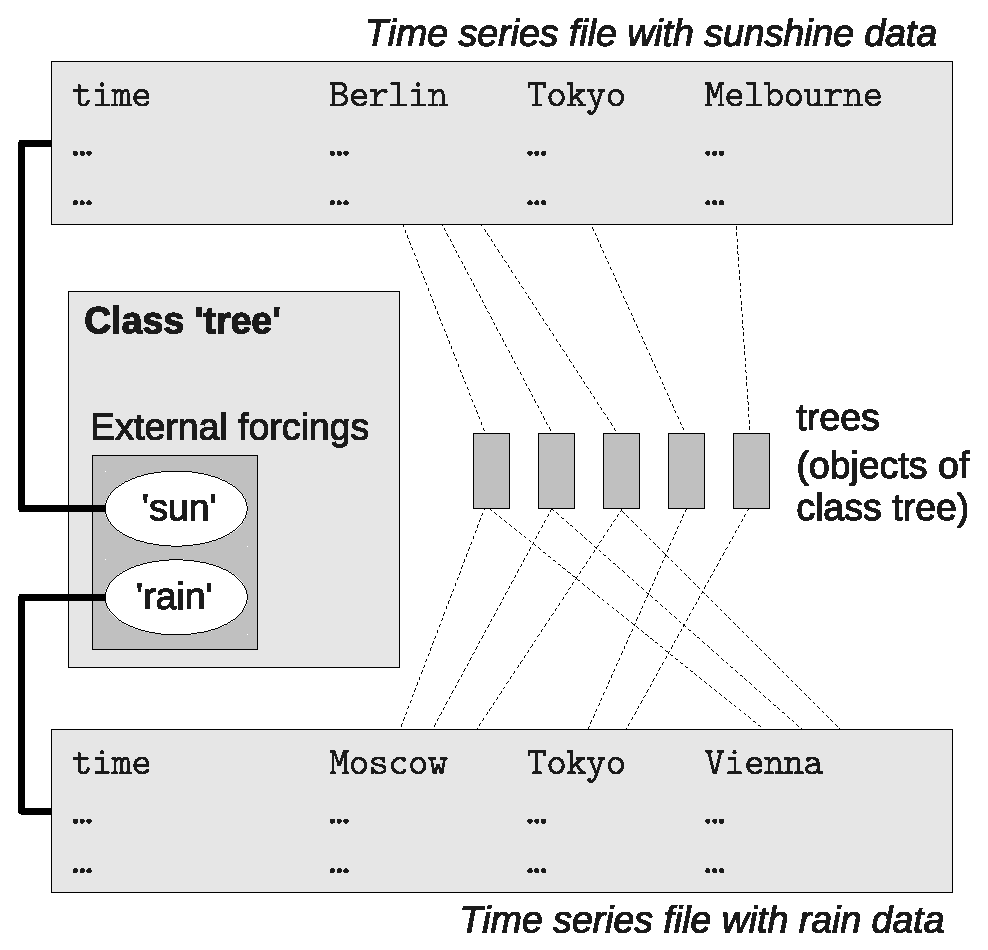
\includegraphics[width=0.9\columnwidth]{\figdir/externalForcingsManagement_overview.eps}
  \caption{Example illustrating the assignment of external forcings to objects of a particular class. \label{fig:input-external-overview}}
\end{figure}

To make this strategy work, two things have to be done:
\begin{enumerate}
  \item The two external input variables of the 'tree' class have to be linked with two time series files, containing the actual data for a single variable at all available stations. This is illustrated by the solid connecting lines in \figref{fig:input-external-overview}. The model's input file that is used to establish those links between variables and time series files is described in \secref{sec:input-externalVariables}.
  \item Links must also be established between the individual objects and the locations (\ie{} climate stations). This is illustrated by the dashed connecting lines in \figref{fig:input-external-overview}. Such links exist separately for each external forcing. Since a single object may be linked to more than one location, the links must also have a 'weight' attribute. This allows to account for the fact that Berlin is nearer to Vienna than to Moscow, when the rainfall for Berlin is estimated. The model's input file that is used to establish the links between objects and locations is described in \secref{sec:input-externalLocations}.
\end{enumerate}

%%%%%%%%%%%%%%%%%%%%%%%%%%%%%%%%%%%%%%%%%%%%%%%%%%%%%%%%%%%%%%%%%%%%%%%%%%%%%%%%
\subsection{Time series data files} \label{sec:input-timeseries}

A time series\index{time series} data file is a table with the usual header and \emph{two or more} columns. As an exception to the usual convention (see \secref{sec:input-formats}), the time information must always be present in the \emph{first} column of the table. The remaining $n$ column(s) contain the time-dependend values of the respective variable at $n$ locations. The order of these remaining columns is arbitrary since they are identified by their column names (which usually represent location names/IDs). The name of the first column containg the time information must be present but it is ignored. A reasonable name would be the abbreviation of the respective time zone, such as 'UTC'. An example of a time series data file is given in \figref{fig:input-timeseries}.

\begin{figure*}[htbp]
  \lstinputlisting[style=txt]{\figdir/example_timeseries.txt}
  \caption{Example of time series data file containing values of a variable at three locations. \label{fig:input-timeseries}}
\end{figure*}

The entries in the time column (first column), must comply with the subsequent rules:
\begin{itemize}
  \item Times must be encoded as stings in ISO 8601 format (\verb!YYYY-MM-DD hh:mm:ss!) as already described in \secref{sec:input-formats}. Due to this format, the highest possible resolution is 1 second.
  \item Any character can be used to separate date and time information (blank is a usual convention). It may even be identical with a character used to separate the table columns.
  \item The times must be in \emph{strictly} increasing order, \ie{} the latest data are expected in the file's first record and there must be no duplicate times.
  \item Regular as well as irregular time series are supported, \ie{} the time differences between neighbored records may be variable within a file. This offers the chance to use a higher resolution in periods of increased data variability and to use a low resolution when the values change slowly (or not at all). Such a strategy can save disk space and reduce the effort for reading data.
  \item The resolution, \ie{} the smallest time differences between \emph{any} neighbored records must be $\geq$ the simulation time step (see keyword \verb!delta_t! in \tabref{tab:config-time}). To give an example: If the simulation time step is 1 hour (\verb!delta_t=3600!), one can use time series with a minimum resolution of 1 hour or more (\ie{} 1 hour, 2 hours, 1 day, 3 days, etc.). A time series file containing (some/only) 5 minute data, for example, will not be accepted.
  \item If the resolution of the time series data file $\Delta t$ differs (for some or all interval(s)) from the simulation time step \verb!delta_t!, the values are automatically transformed (\ie{} reduced) if they represent sums (see discussion of column \verb!sums! in \secref{sec:input-externalVariables}).
\end{itemize}

With respect to the data values, the following restrictions apply:
\begin{itemize}
  \item The values always represent averages or sums over a certain time interval (\ie{} they do not represent instantaneous values). The respective time interval is determined by the difference in times between two neighbored records (see discussion of column \verb!past! in \secref{sec:input-externalVariables} for details).
  \item Missing values or special values used to identify invalid data (such as \verb!NA!) are \emph{not} supported. Thus, data gaps must be handled by external software (or manual work) prior to model application. It is possible, however, to use special numerical values (often -9999) to mark missing/invalid data and to treat them properly in the classes' simulate methods.
\end{itemize}

%%%%%%%%%%%%%%%%%%%%%%%%%%%%%%%%%%%%%%%%%%%%%%%%%%%%%%%%%%%%%%%%%%%%%%%%%%%%%%%%
\subsection{Assignment of time series files and attributes to variables} \label{sec:input-externalVariables}

Each external input variable\index{external input} which has been declared for a particular object class must be linked to a time series file. The time series file contains the actual data and its format is described in \secref{sec:input-timeseries}. In addition to that, a time series has further attributes which describe how the times and values are to be interpreted.

All information on the linkage of variables and time series files as well as time series attributes hast to be supplied in a single table with the following four columns:

\begin{columndef}
  \item [variable] (\textit{string}) Names of the external input variables.
  \item [file] (\textit{string}) Names of the files containing the time series data for an external input variable (see \secref{sec:input-timeseries} for details on the format and restrictions).
  \item [sums] (\textit{logical}) If \true{}, the data value related to a particular time interval is interpreted as a sum. This is appropriate for data generally measured as sums. Examples include precipitation (given in units of mm/interval) or radiation (if expressed in units of Joule/interval). If \false{}, the data are interpreted as averages over the time interval. This is appropriate, for example in case of velocities (m/s) and the like, temperatures, or radiation intensities (expressed in units of Watts).
  \item [past] (\textit{logical}) It is a common practice that time series data files contain a single time column only, even if the stored values represent averages or sums over time intervals instead of instantaneous values (see \secref{sec:input-timeseries}). Consequently, there must be a convention whether a given time marks the \emph{begin} or the \emph{end} of an interval. This is accomplished through the setting of \verb!past!. If \verb!past=true!, it is assumed that the times given in the respective column of a time series data file mark \emph{end-of-intervals}. This is a intuitive convention used by many (but not all) data providers. It is important to note that the begin of the time interval related to the very first record in the file is \emph{unknown} if \verb!past=true!. Consequently, the data values of the very first record are ignored. In contrast to that, times given in the time series file are assumed to mark the begin of time intervals, if \verb!past=false!. Then, the end of the time interval related to the last record in the file is unknown and the values are, consequently, ignored. See also \figref{fig:input-timeseries} for an example.
\end{columndef}

Note that the table does \emph{not} contain a column like \verb!objectGroup!. Thus, if an external input variable with the same name is declared in multiple object classes, the data are always taken from the same time series file. Thus, the table should contain as many records as there are unique names of external input variables in all object classes. An example of a simple table is provided in \figref{fig:input-externalVariables}.

\begin{figure*}[htbp]
  \lstinputlisting[style=txt]{\figdir/example_externalVariables.txt}
  \caption{Example of table holding information on time series data files and attributes for a set of external input variables. \label{fig:input-externalVariables}}
\end{figure*}

%%%%%%%%%%%%%%%%%%%%%%%%%%%%%%%%%%%%%%%%%%%%%%%%%%%%%%%%%%%%%%%%%%%%%%%%%%%%%%%%
\subsection{Assignment of external input locations to objects} \label{sec:input-externalLocations}

The table used to establish the links between objects and certain columns of a time series data file (that usually represent different locations) consists of the four colums described below:

\begin{columndef}
  \item [object] (\textit{string}) Names (ID strings) of objects getting external input.
  \item [variable] (\textit{string}) Names of the external input variable(s).
  \item [location] (\textit{string}) Location(s) to be assigned to a particular variable for a particular object. The used location name must be an existing column in the time series data linked to the respective variable (see \secref{sec:input-externalVariables}).
  \item [weight] (\textit{numeric}) Weights to be assigned to a particular station for a particular variable and object. If, for a specific variable, an object uses data from only a single location, the weight is generally 1.0. If, for a specific variable, the object is linked to multiple stations, the \emph{sum of weights} over all locations (for that variable) is 1.0. This is just the usual case of spatial interpolation or, more generally, weighted averaging (see \eqnref{eqn:input-externalLocationWeights}).
\end{columndef}

The value of an external forcing\index{external input} applied to a particular object at a particular time, $X$ is computed according to \eqnref{eqn:input-externalLocationWeights}. In this equation, $w_i$ is the weight of a location with index $i$ as assigned in the \verb!weight! column of the described table. The symbol $v_i$ denotes the value of the external variable for the same location (index $i$) read from the respective time series data file. The number of involved locations is $n$.

\begin{equation}
  \label{eqn:input-externalLocationWeights}
  X = \sum_{i=1}^{n} w_i \cdot v_i
\end{equation}

The described weighting approach and its typical use in the context of spatial interpolation is illustrated by \figref{fig:input-externalLocationWeights}. In the shown cases (a) and (b), the number of involved locations $n$ with respect to a particular object and variable is 1 and the assigned weight $w_1$ equals 1.0. In the cases (c) and (d) we have $n>1$ and multiple weights whose values satisfy \eqnref{eqn:input-externalLocationWeights}.

\begin{figure}[htbp]
  \centering
  \begin{tabular}{cc}
  (a) & (b) \\
  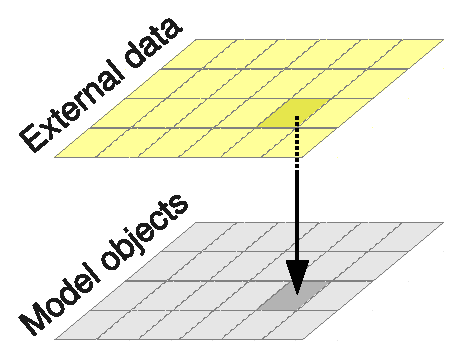
\includegraphics[width=0.45\columnwidth]{\figdir/externalinputs_weights_a.eps} &
  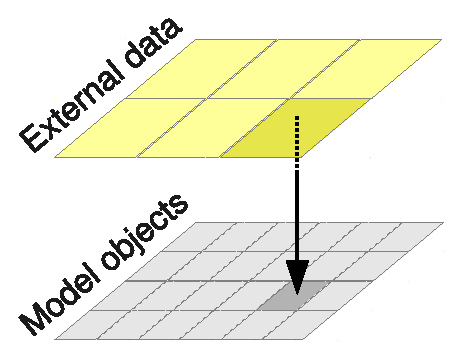
\includegraphics[width=0.45\columnwidth]{\figdir/externalinputs_weights_b.eps} \\
  (c) & (d) \\
  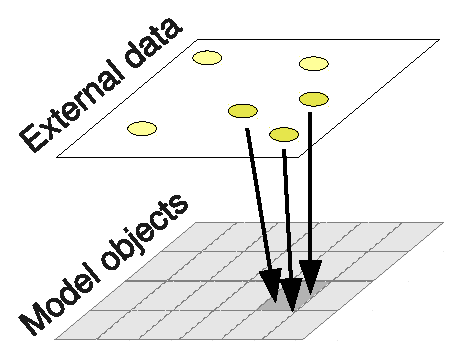
\includegraphics[width=0.45\columnwidth]{\figdir/externalinputs_weights_c.eps} &
  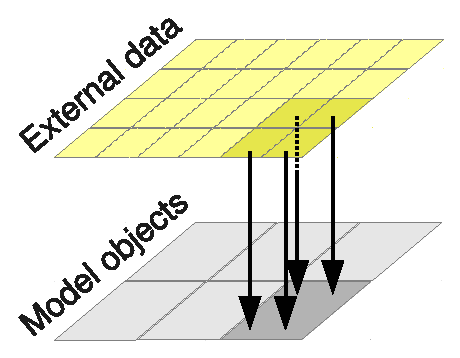
\includegraphics[width=0.45\columnwidth]{\figdir/externalinputs_weights_d.eps} \\
  \end{tabular}
  \caption[Assignment of values of an external variable measured at multiple locations to the simulated objects.]{Assignment of values of an external variable measured at multiple locations to the simulated objects (here represented by grid cells). Shown are typical situations arising in spatially distributed modeling: (a) Spatial resolution of the external variable matches with the model's resolution, (b) Use of low-resolution input in a high-resolution model, (c) Estimation of an object's input by interpolation of point data, (d) Use of high-resolution data in a low-resolution model. \label{fig:input-externalLocationWeights}}
\end{figure}

A minimum example of a table assigning external input locations to objects is given in \figref{fig:input-externalLocations}. This table corresponds to the example introduced in \secref{sec:input-external-overview}. In realistic, more complex models, such a table may become quite large, especially if many objects are simulated that use information of multiple external input variables and the input (for a specific object and variable) is taken from multiple locations. This is due to the fact that the information for all objects (of all classes) is collected in a single table.

\begin{figure*}[htbp]
  \lstinputlisting[style=txt]{\figdir/example_externalLocations.txt}
  \caption[Example of table holding information on the links between the simulated objects and the locations where data of external input variables are available.]{Example of table holding information on the links between the simulated objects and the locations where data of external input variables are available. The table corresponds to the example used in \secref{sec:input-external-overview} (\figref{fig:input-external-overview}). \label{fig:input-externalLocations}}
\end{figure*}

%%%%%%%%%%%%%%%%%%%%%%%%%%%%%%%%%%%%%%%%%%%%%%%%%%%%%%%%%%%%%%%%%%%%%%%%%%%%%%%%
%%%%%%%%%%%%%%%%%%%%%%%%%%%%%%%%%%%%%%%%%%%%%%%%%%%%%%%%%%%%%%%%%%%%%%%%%%%%%%%%
%%%%%%%%%%%%%%%%%%%%%%%%%%%%%%%%%%%%%%%%%%%%%%%%%%%%%%%%%%%%%%%%%%%%%%%%%%%%%%%%

\FloatBarrier

\section{Initialization of states} \index{state variable!initialization}

%%%%%%%%%%%%%%%%%%%%%%%%%%%%%%%%%%%%%%%%%%%%%%%%%%%%%%%%%%%%%%%%%%%%%%%%%%%%%%%%
\subsection{Initialization table for scalar states} \label{sec:input-initScal}

This table contains the initial values of all the scalar state variables of all simulated objects (see \figref{fig:input-initScal} for an example). The three required columns are defined as follows:

\begin{columndef}
  \item [object] (\textit{string}) Names (ID strings) of all objects with one or more scalar state variable(s).
  \item [variable] (\textit{string}) Names of the scalar state variable(s).
  \item [value] (\textit{numeric}) Initial values assigned to the corresponding variables of the respective models.
\end{columndef}

\begin{figure*}[htbp]
  \lstinputlisting[style=txt]{\figdir/example_initScal.txt}
  \caption{Example of table with initial values of scalar state variables. \label{fig:input-initScal}}
\end{figure*}

%%%%%%%%%%%%%%%%%%%%%%%%%%%%%%%%%%%%%%%%%%%%%%%%%%%%%%%%%%%%%%%%%%%%%%%%%%%%%%%%
\subsection{Initialization table for vector states} \label{sec:input-initVect}

As opposed to the initialization table for scalar state variables (see \secref{sec:input-initScal}), the initialization table for vector state variables has an additional column named \verb!index!. This column is of type \textit{integer} and contains the element indices corresponding to the vector state variable specified in the \verb!variable! column. The following rules apply to the \verb!index! column:
\begin{itemize}
  \item The C/C++ convention is used for the vectors' indices, \ie{} the index of a vector's first element is 0 (not 1, as in many other programming languages).
  \item For each model and variable, at least one record must be present with a value of 0 in the \verb!index! column. Thus, an initial value must be present at least for one (the first) element of each vector.
  \item More records may follow for a particular model and variable, with values of 1 through $n$ in the index column. The index values must increase by 1 from one record to the next, \ie{} there must be no gaps in the sequence of indices.
  \item The highest index value, $n$, determines the \emph{initial size} of a vector. Since indexing starts at 0, the total vector size (number of elements) is $n-1$. Note that a vector's size may change during simulation, depending on the code of the simulate method of the corresponding model class.
\end{itemize}

A simple example of an initialization table for vector state variables is given in \figref{fig:input-initVect}.

\begin{figure*}[htbp]
  \lstinputlisting[style=txt]{\figdir/example_initVect.txt}
  \caption[Layout of a table with initial values of vector state variables.]{Layout of a table with initial values of vector state variables. The example corresponds to a model of apple trees having a variable number of fruits. Consequently, all properties of the individual apples must be held in vector state variables. Initially, the apple tree 'tree1' has three fruits and 'tree2' has only two. Depending on the implementation of the apple tree class, these numbers may change during simulation.
 \label{fig:input-initVect}}
\end{figure*}

%%%%%%%%%%%%%%%%%%%%%%%%%%%%%%%%%%%%%%%%%%%%%%%%%%%%%%%%%%%%%%%%%%%%%%%%%%%%%%%%
%%%%%%%%%%%%%%%%%%%%%%%%%%%%%%%%%%%%%%%%%%%%%%%%%%%%%%%%%%%%%%%%%%%%%%%%%%%%%%%%
%%%%%%%%%%%%%%%%%%%%%%%%%%%%%%%%%%%%%%%%%%%%%%%%%%%%%%%%%%%%%%%%%%%%%%%%%%%%%%%%

\FloatBarrier

\section{Model output control} \index{output}

%%%%%%%%%%%%%%%%%%%%%%%%%%%%%%%%%%%%%%%%%%%%%%%%%%%%%%%%%%%%%%%%%%%%%%%%%%%%%%%%
\subsection{Selecting output variables for specific objects} \label{sec:input-outputSelected} \index{output!selection}

For each object, the output of simulated values in the form of time series may be requested. Note that this is restricted to those variables which have been declared as 'outputs' in the corresponding class. Consequently, if time series output for a state variable is required, for example, one must declare an (additional) output variable in the respective object class and the values of the state variable must be assigned to the output variable in each time step. The same procedure is necessary in order to output time series of an object's external inputs, functions, etc. The table used to request output of certain variables for certain objects has the following two columns:

\begin{columndef}
  \item [object] (\textit{string}) Names (ID strings) of objects for which output is requested.
  \item [variable] (\textit{string}) Names of output variables declared in the classes corresponding to the objects. A separate record is expected for each variable.
  \item [digits] (\textit{integer}) Controls the number of digits after the decimal place. Numbers are always printed in a fixed format, \ie{} as 0.33 instread of 3.3e-01, for example.
\end{columndef}

An example of such a table is given in \figref{fig:input-outputSelected}. It is important to note that it is \emph{not} checked whether the entries in the \verb!object! column actually represent the names of existing objects. Thus, to turn off \verb!any! output, one could just supply a single record with a non-existing object's name.

\begin{figure*}[htbp]
  \lstinputlisting[style=txt]{\figdir/example_outputSelected.txt}
  \caption{Example of a table used to request the writing of time series files for selected output variables of certain models.
 \label{fig:input-outputSelected}}
\end{figure*}

Also note that the time series of all variables requested for a particular object are written to a single file. The name of this file is generated automatically by appending an extension (determined by the requested format) to the object's name. The directory where the output file will appear is controlled by the value assigned to key \verb!outputDirectory! in the configuration file (see \tabref{tab:config-output}).

%%%%%%%%%%%%%%%%%%%%%%%%%%%%%%%%%%%%%%%%%%%%%%%%%%%%%%%%%%%%%%%%%%%%%%%%%%%%%%%%
\subsection{Enabling debug output for specific objects} \label{sec:input-outputDebug} \index{output!debug}

By requesting debug output for certain objects, it is possible to create time series outputs for basically \emph{all} computed values, namely
\begin{itemize}
  \item Scalar state variables
  \item Vector state variables
  \item External input variables
  \item Simulated input variables
  \item Output variables.
\end{itemize}

This kind of output is particularly useful when debugging a model. Depending on the complexity of an object's data and the number of simulated time steps, the produced output files may become quite large. Therefore, the approach described in \secref{sec:input-outputSelected} is usually more appropriate if only some of the computed quantities are actually of interest.

The table used to request debug outputs consists of just a single column with name \verb!object! (no example given). It holds the names (ID strings) of the objects for which output is requested. It is \emph{not} checked whether the entries in that column represent the names of existing objects. Thus, if no debug output is required at all, the table should contain just a single record with a non-existing object's name. Note that the writing of large debug output files that are not actually required may lead to a significant waste of computing time and disk space.

The name(s) of the output file(s) are generated automatically by appending an extension (currently \texttt{.dbg}) to the objects' name(s). The directory where the output files will appear is controlled by the value assigned to key \verb!outputDirectory! in the configuration file (see \tabref{tab:config-output}).

%%%%%%%%%%%%%%%%%%%%%%%%%%%%%%%%%%%%%%%%%%%%%%%%%%%%%%%%%%%%%%%%%%%%%%%%%%%%%%%%
\subsection{Output of the model's state at selected times}  \label{sec:input-outputState} \index{output!model state}

In some situation is is desirable to write the values of all state variables of all simulated \emph{at a certain point in time} to disk. Potential uses of the produced file(s) containing the \emph{entire model's state} include
\begin{itemize}
  \item restarting of the model, using the produced files to initialize the state variables in a subsequent call,
  \item visualization of spatial patterns.
\end{itemize}

The table used to request outputs of the model's state consists of just a single column with name \verb!time! (no example given). It holds the times for which the output is requested as strings in the usual ISO 8601 format (see \secref{sec:input-formats}). One should note that output is only created if a specified time also represents the end of a simulation time step (exactly to the second). Thus, it is not possible to request the model's state for intermediate times (such as 07:30, if the simulation time step is 1 hour and the model was started at a full hour).
The only technique of suppressing outputs of the model's state at all is to specify (valid) times that do not meet the above criteria. Preferably, one specifies just a single time which is far outside the simulation time window and easily identified as a dummy such as \verb!1900-01-01 00:00:00!, for example. Saving state information for many time steps despite of the fact that it is not actually required wastes both computing time and disk space.

For each point in time, two output files are created. One of the files contains the current values of scalar state variables and the other file holds the values of the vector state variables. The used formats are identical to the initialization tables described in \secref{sec:input-initScal} (\figref{fig:input-initScal}) and \secref{sec:input-initVect} (\figref{fig:input-initVect}), respectively.

The name(s) of the output file(s) are generated automatically using the respective time stamp. The values of the scalar state variables are saved in file \verb!statesScal_YYYYMMDDhhmmss! and the vector state variables are written to file \verb!statesVect_YYYYMMDDhhmmss!.The 14 digits at the end of the file names encode the time (4-digit year, followed by 2-digit month, day, hour, minute, and second). The directory where the output files will appear is controlled by the value assigned to key \verb!outputDirectory! in the configuration file (see \tabref{tab:config-output}).

%%%%%%%%%%%%%%%%%%%%%%%%%%%%%%%%%%%%%%%%%%%%%%%%%%%%%%%%%%%%%%%%%%%%%%%%%%%%%%%%
\subsection{Precision of printed outputs}  \label{sec:input-outputPrecision} \index{output!precision}

The current version of the \software{echse} writes all output data in a scientific format with three digits after the period. Thus, numbers are formatted like \texttt{$\pm$X.YYYe$\pm$ZZ}, where \texttt{ZZ} is the exponent (base 10) corresponding to the number \texttt{X.YYY}. Currently, the output format \emph{cannot} be changed by the model user.

A potential issue with the \texttt{$\pm$X.YYYe$\pm$ZZ} format is that the precision of output data is limited to a total number of 4 digits. This is sufficient for many applications but may sometimes be problematic. In such cases, it is recommended to transform the data by adding or subtracting an appropriate constant (at latest before calling the \verb!set_output()! method; see \tabref{tab:concept-dataAccessFunctions_write}).

Let's consider the example of a reservoir in a mountainous region. Suppose that the reservoir's water level ranges from 2150 to 2180 m (a.s.l.) due to operation and fluctuations of the inflow. If the model writes the simulated water level to output files in units of m a.s.l., the precision is limited to 1~m only! To notice that, one must consider that the minimum and maximum values would be printed as \texttt{2.150e+03} and \texttt{2.180e+03}, respectively. By subtracting an appropriate constant, say 2100, the output precision can be increased significantly because the new data range is 50--80 (printed as \texttt{5.000e+01} and \texttt{8.000e+01}, respectively). After the transformation, the precision of the printed data is about 1~cm, \ie{} 100 times higher.

\chapter{User guidelines} \label{chap:guidelines}
\renewcommand{\tabdir}{chapters/guidelines/tab}
\renewcommand{\figdir}{chapters/guidelines/fig}

%%%%%%%%%%%%%%%%%%%%%%%%%%%%%%%%%%%%%%%%%%%%%%%%%%%%%%%%%%%%%%%%%%%%%%%%%%%%%%%%
%%%%%%%%%%%%%%%%%%%%%%%%%%%%%%%%%%%%%%%%%%%%%%%%%%%%%%%%%%%%%%%%%%%%%%%%%%%%%%%%
%%%%%%%%%%%%%%%%%%%%%%%%%%%%%%%%%%%%%%%%%%%%%%%%%%%%%%%%%%%%%%%%%%%%%%%%%%%%%%%%
\section{Model discretization} \label{sec:guidelines-discretization}

Often, alternative options of discretizing a real-world system do exist. Each alternative usually comes with specific pros and cons. Depending in the intended application of the model, a particular option may be more or less appropriate (or convienient to use). Basic aspects of proper model discretization are discussed in the subsequent sections \secref{sec:guidelines-discretization-basic}--\ref{sec:guidelines-discretization-sub}.

\subsection{Basic rule} \label{sec:guidelines-discretization-basic}

The most basic rule is this: If two objects are charavcterized by different sets of state variables, \ie{} the names of the state variables are not the same, the two objects belong to different classes.

\subsection{Sub-discretization} \label{sec:guidelines-discretization-sub}

Real-world objects can (or must be) often further discretized into sub-units. This is usually the case, when the object's state variables are subject to spatially variability. For example, a larger catchment can be broken into sub-catchments, that differ with respect to certain properties (proportion of forest, soil type, etc.). In such situations one has to decide whether the sub-discretization should implemented
\begin{itemize}
  \item within the object, or
  \item by splitting an object into multiple separate objects.
\end{itemize}

Such a decision should be made based on the guidelines presented below.

\subsubsection{Dynamic sub-discretization}
If the sub-discretization (\ie{} the number of spatial sub-units, for example) is time-variable, one must use vector-valued state variables (see \secref{sec:concept-classFeatures-states}). This is due to the fact that the size (\ie{} the number of elements) of the vectors is allowed to change during the simulation period. A dynamic sub-discretization may be necessary when modeling the travelling of a flood wave in a homogeneous river reach represented by a cascade of linear reservoirs. In such a model, the appropriate number of linear reservoirs typically depends on the flow rate.

The approach of using vector-valued state variables only introduces additional state variables (but not parameters, etc.). Note: Pragmatically, vector state variables may also be 'misused' as scalar parameters, if parameter values are variable among the sub-units. This is, however, not efficient, because the info on parameters then (unnecessarily) appears in output files.

\subsubsection{Static Sub-Discretization}
If, in contrast to the situation discussed above, the number of sub-units is constant over the simulation period, several alternatives do exist:

\paragraph{State variables only} If the sub-discretization is limited to state variables (\ie{} all sub-units have common parameters and external inputs), one may use vector-valued state variables. The size of the vectors is simply held constant (by not changing it). Note: Pragmatically, vector state variables may also be 'misused' as scalar parameters, if parameter values are variable among the sub-units. This is, however, not efficient, because the info on parameters then (unnecessarily) appears in output files.

\paragraph{Fixed number of sub-units} If the number of sub-units is the same for all objects of a class, one should use multiple scalar state variables (and/or parameters). Example: A catchment class, with a fixed number of land-use classes (such as 'forest', 'water', 'urban', 'other').

\paragraph{Remaining cases} If (a) the sub-discretization is not limited to state variables (\ie{} parameters are variable as well) and (b) the number of required sub-units is specific to individual objects, one should treat the sub-units as objects of a separate (additional) class and define appropriate interactions between the objects of the original and new class. Example: If the number of (relevant) land-uses in a catchment varies from one catchment to the next (and using a fixed number seems inefficient), one may introduce a class new 'landUseUnit'. The sub-units are then implemented as objects of that new class, each being linked to the corresponding catchment object.

%%%%%%%%%%%%%%%%%%%%%%%%%%%%%%%%%%%%%%%%%%%%%%%%%%%%%%%%%%%%%%%%%%%%%%%%%%%%%%%%
%%%%%%%%%%%%%%%%%%%%%%%%%%%%%%%%%%%%%%%%%%%%%%%%%%%%%%%%%%%%%%%%%%%%%%%%%%%%%%%%
%%%%%%%%%%%%%%%%%%%%%%%%%%%%%%%%%%%%%%%%%%%%%%%%%%%%%%%%%%%%%%%%%%%%%%%%%%%%%%%%
\section{Optimizing for speed} \label{sec:guidelines-speedOptim}

\subsection{Parallel processing} \label{sec:guidelines-speedOptim-parallel}
The \software{echse} software comes with built-in support for \emph{shared-memory} parallel computing. This is implemented using OpenMP (\url{http://openmp.org/}) which is supported by many modern compilers.
Parallel processing can be enabled/disabled by the user via a model's configuration data (see \tabref{tab:config-compuational}).

Please note that \emph{shared-memory} parallel computing only works on systems which are capable of running a \emph{single process} as \emph{multiple threads}. Please note, however, that the attempt to use multi-threading does not necessarily increase the performance, \ie{} save computation time. In fact, depending on computer architecture (hardware) and the specific model, the model may \emph{slow down} unexpectedly although it should become faster from theory. A possible reasons for this undesired behaviour might be that the overhead for the creation of multiple threads is higher than the actual gain from the parallel simulation. Another possible cause might be that, although the machine supports multiple threads, these threads share a limited ressource (like a floating-point arithmetic module, for example). Then, the multiple threads run sequentially in fact.

Present experience has shown that parallel processing is effective on a true multi-processor machine, \ie{} a machine with more than one physical CPU\footnote{Dell machine with 4 CPUs of type Intel Core i7-2620M, each of which with 2 kernels, running 32 bit Ubuntu 12.04 LTS}. It was found to be counterproductive, however, on multi-kernel architectures where all kernels are part of one single CPU\footnote{Several dual-core and quad-core machines running Windows 7}.

Thus, it is recommended to always empirically determine the gain in computation speed (or slow down). This is easily done by inspecting the computation time of a particular simulation with multi-threading being turned on and off, respectively (see \tabref{tab:config-compuational}).
  
\subsection{Miscellaneous} \label{sec:guidelines-speedOptim-misc}
Declaring local variables of the simulate-Method as static does not have an effect (at least when compiling with gcc and optimization). It seems that the optimization performed by the compiler prevents the repeated allocation of memory on every call of the simulate-method.

\chapter{Source code (PRELIMINARY)} \label{chap:code}
\renewcommand{\tabdir}{chapters/code/tab}
\renewcommand{\figdir}{chapters/code/fig}

\section{Programming language} \label{sec:code-language}

Execution time is critical for many operatinal and scientific applications. Therefore, the use of a compiled language (like FORTRAN 95+ or C++) is preferred over the use of a interpreted language (like Java, Matlab, R, $\ldots$). C++ was selected as the language for implementing \software{echse} for the following reasons:

\begin{itemize}
  \item Execution speed of the compiled code.
  \item Full support of object-oriented (OO) programming features.
  \item A standard way of exception handling exists.
  \item Availability of libraries.
  \item Availability of free compilers for any platform (gcc).
  \item Widespread use.
\end{itemize}

%The \software{echse}-code profits from an OO programming style, because it allows for
%\begin{itemize}
%  \item KAPSELUNG: Protection of an object's data against unallowed access.
%  \item VERERBUNG: Handling of objects which differ in its data or methods by using the common base class. For example, a base class 'hydrologicElement' may be defined with the child classes 'lake' and 'watershed'. Say \emph{three} lakes and \emph{five} watersheds are instantiated during runtime. Because lakes and watersheds ar all 'hydrologic elements' (\ie{} they have a common base class) we can easily iterate over all \emph{eigth} objects. We call the common methods defined in the base classes, which are overloaded in the child classes.
%\end{itemize}

% Why using exceptions?
%(1) Werden keine Exceptions verwendet (wie etwa in Fortran oder C), muss jede Methode einen Statuswert (z.B. integer) an die aufrufende Umgebung liefern. Dieser muss dann jeweils in der aufrufenden Umgebung kontrolliert werden. Unterbleibt die Kontrolle, verliert sich das Programm leicht in einem undeinierten Zustand. Werden dagegen Exceptions verwendet, ist ein definiertes Programmende garantiert, auch dann, wenn der Fehler nicht in der aufrufenden Einheit behandelt wird (was er aber sollte).
%(2) Wird eine Exception ausgelöst, wird dynamisch alloziierter Speicher automatisch freigegeben.
%(3) Mit Exceptions lässt sich relativ leicht ein traceback erstellen (geht aber auch ohne).


%%%%%%%%%%%%%%%%%%%%%%%%%%%%%%%%%%%%%%%%%%%%%%%%%%%%%%%%%%
%%%%%%%%%%%%%%%%%%%%% LISTS %%%%%%%%%%%%%%%%%%%%%%%%%%%%%%
%%%%%%%%%%%%%%%%%%%%%%%%%%%%%%%%%%%%%%%%%%%%%%%%%%%%%%%%%%
\clearpage
\fancyhead[LE,RO]{\bfseries\thepage}
\fancyhead[RE]{\bfseries List of figures}
\fancyhead[LO]{\bfseries List of figures}
\addcontentsline{toc}{chapter}{List of figures}
\listoffigures

\clearpage
\fancyhead[LE,RO]{\bfseries\thepage}
\fancyhead[RE]{\bfseries List of tables}
\fancyhead[LO]{\bfseries List of tables}
\addcontentsline{toc}{chapter}{List of tables}
\listoftables

%%%%%%%%%%%%%%%%%%%%%%%%%%%%%%%%%%%%%%%%%%%%%%%%%%%%%%%%%%
%%%%%%%%%%%%%%%%%%%%% BIBLIOGRAPHY %%%%%%%%%%%%%%%%%%%%%%%
%%%%%%%%%%%%%%%%%%%%%%%%%%%%%%%%%%%%%%%%%%%%%%%%%%%%%%%%%%
\clearpage
\fancyhead[LE,RO]{\bfseries\thepage}
\fancyhead[RE]{\bfseries Bibliography}
\fancyhead[LO]{}
\addcontentsline{toc}{chapter}{Bibliography}
\bibliographystyle{../../_common/elsarticle-harv}
\bibliography{/home/dkneis/literature/jabref/bib_hydrologicalModeling,/home/dkneis/literature/jabref/bib_diplomaAndDiss}

%%%%%%%%%%%%%%%%%%%%%%%%%%%%%%%%%%%%%%%%%%%%%%%%%%%%%%%%%%
%%%%%%%%%%%%%%%%%%%%% THE APPENDIX %%%%%%%%%%%%%%%%%%%%%%%
%%%%%%%%%%%%%%%%%%%%%%%%%%%%%%%%%%%%%%%%%%%%%%%%%%%%%%%%%%

\chaptermark{A}
\clearpage
\fancyhead[LE,RO]{\bfseries\thepage}
\fancyhead[RE]{\bfseries Appendix}
\fancyhead[LO]{}
\addcontentsline{toc}{chapter}{Appendix}
\appendix
%
\chapter{Installation of model engines} \label{chap:install}
\renewcommand{\tabdir}{chapters/install/install/tab}
\renewcommand{\figdir}{chapters/install/install/fig}

\section{Introduction} \label{sec:install:intro}

This chapter deals with the installation of \software{echse}-based model engines from \emph{existing} source code. The chapter does not cover the topic of model development or modification. The information is addressed to users of both Linux and Windows.

In this context, the term \emph{model engine} is used to denote the binary file which is executed when performing a simulation. The term is introduced to allow for a clear distinction between the \emph{model engine} (plain binary file) and the \emph{model} (binary file + input data). 

%%%%%%%%%%%%%%%%%%%%%%%%%%%%%%%%%%%%%%%%%%%%%%%%%%%%%%%%%%%%%%%%%%%%%%%%%%%%%%
%%%%%%%%%%%%%%%%%%%%%%%%%%%%%%%%%%%%%%%%%%%%%%%%%%%%%%%%%%%%%%%%%%%%%%%%%%%%%%

\section{Software to install} \label{sec:install:software}

%%%%%%%%%%%%%%%%%%%%%%%%%%%%%%%%%%%%%%%%%%%%%%%%%%%%%%%%%%%%%%%%%%%%%%%%%%%%%%

\subsection{Programs}

You need to install the following programs in order to build an \software{echse}-based model engine:

\begin{itemize}
  \item The 'R' software for statistical computing.
  \item The GNU C++ compiler 'g++'.
  \item Windows users: The bash-shell interpreter and commands provided by 'MSYS'.
\end{itemize}

Linux users probably want to use the package manager to install the software. Windows users should try the installers which can be downloaded from the respective websites. Please follow the installation instructions given in \chapref{chap:extSoft} as closely as possible. In particular, on Windows systems, it is important to add the binary directories of all the software to the \verb!PATH! variable in order to make the programs accessible from any shell.

%%%%%%%%%%%%%%%%%%%%%%%%%%%%%%%%%%%%%%%%%%%%%%%%%%%%%%%%%%%%%%%%%%%%%%%%%%%%%%

\subsection{R-packages}

You need to install the R-package \software{codegen} in order to run the \software{echse}'s code generator. You should find the latest version of this package in the sub-folder \verb!R/packages! of the \software{echse}-tools main directory (see \secref{sec:install:folders}). The package is distributed as a tarball archive \verb!codegen_x.y.tar.gz! where \verb!x.y! is the current version number. See \secref{sec:extSoft:R:packages} for details on how to install R-packages.

%%%%%%%%%%%%%%%%%%%%%%%%%%%%%%%%%%%%%%%%%%%%%%%%%%%%%%%%%%%%%%%%%%%%%%%%%%%%%%
%%%%%%%%%%%%%%%%%%%%%%%%%%%%%%%%%%%%%%%%%%%%%%%%%%%%%%%%%%%%%%%%%%%%%%%%%%%%%%

\section{The \software{echse} standard folders} \label{sec:install:folders}

%%%%%%%%%%%%%%%%%%%%%%%%%%%%%%%%%%%%%%%%%%%%%%%%%%%%%%%%%%%%%%%%%%%%%%%%%%%%%%

\subsection{Overview} \label{sec:install:folders:overview}

At present, all \software{echse}-related files are split accross a small number of folders, also referred to as the \software{echse} \emph{standard folders}. These folders are briefly explained in \tabref{tab:install:folders}.

\begin{table}[h]
  \caption{The \software{echse} standard folders. \label{tab:install:folders}}  
  \begin{tabular}{p{0.2\textwidth}p{0.75\textwidth}} \hline\hline
     Folder & Contents \\ \hline
     \verb!echse_docs! & Documentations, mostly as \LaTeX{} projects. \\
     \verb!echse_generic! & Common C++ source code being used by all \software{echse}-based model engines. Also contains generic scripts for engine building. \\
     \verb!echse_engines! & C++ source code of the classes being used by one or more particular model engines. This includes both generated and manually written code. Also contains text files with class and model declarations. \\
     \verb!echse_tools! & \software{echse}-related tools for pre- and post-processing of data. \\
     \hline\hline
  \end{tabular}
\end{table}

It is assumed that you have obtained current versions of the \software{echse} standard folders listed in \tabref{tab:install:folders} either from repositories or by unpacking release archives. In order to install a model engine, you need at least the \verb!echse_generic! and \verb!echse_engines! folders whose contents is displayed in \figsref{fig:install:folders:generic} \& \ref{fig:install:folders:engines}, respectively. Note that only the most important branches are displayed in these figures.

\begin{figure}[h]
\begin{lstlisting}[style=text]
  echse_generic --+-- core
                  |
                  +-- cpplib
                  |
                  +-- scripts
\end{lstlisting}
  \caption{Main branches of the \software{echse} standard folder with generic files. \label{fig:install:folders:generic}}
\end{figure}

\begin{figure}[h]
\begin{lstlisting}[style=text]
  echse_engines --+-- bin
                  |
                  +-- classes
                  |
                  +-- def
                  |
                  +-- generated
                  |
                  +-- processes
\end{lstlisting}
\caption{Main branches of the \software{echse} standard folder with class files for particular model engines. \label{fig:install:folders:engines}}
\end{figure}

The functionality of many scripts and files contained in the folders \verb!echse_generic! and \verb!echse_engines! and its sub-folders depends on the integrity of the respective directory trees. Therefore, you should \emph{not} rename, move, or delete any of the sub-folders and files without considering the potential consequences. Note that all references to files and directories are \emph{relative}. Therefore, you can savely move each of the \software{echse} standard folders \emph{as a whole} as long as you keep your system informed on their locations (see \secref{sec:install:env:folders}).

%%%%%%%%%%%%%%%%%%%%%%%%%%%%%%%%%%%%%%%%%%%%%%%%%%%%%%%%%%%%%%%%%%%%%%%%%%%%%%

\subsection{Definition of model engines} \label{sec:install:folders:engines}

The following enumeration outlines the concept of model engines from a top-down point of view. It also gives a brief overview of the contents of the \software{echse} standard folder \verb!echse_engines!.

\begin{enumerate}
  \item Each model engine is composed of a particular set of classes. A rainfall-runoff model, for example, may comprise a sub-basin class, a reach class, and additional classes for special types of objects (reservoirs etc.). The set of classes being used in a particular model engines is listed in the text files in folder \verb!echse_engines/def!.
  \item Each of the classes is characterized by a particular set of data members (forcings, state variables, parameters, etc.). For each class, the declaration of data members can be found in the text files in folder \verb!echse_engines/classes/declaration!. See \citet{Echse-Main-Doc} for details.
  \item Class declaration and implementation are well separated. The declaration part of the classes' source code is created by the code generator (output in \verb!echse_engines/generated!). The implementation part consisting of manually written code to be found in \verb!echse_engines/classes/implementation! (C++ include files).
  \item The dynamics of state variables are due to the action of processes. In the \software{echse} concept, processes are represented by functions whose return value is typically a rate (mass or energy flux) or a derivative of a state variable with respect to time. Since a particular function may be used in multiple classes, the code is separated from the class implementation. It can be found in \verb!echse_engines/processes!
\end{enumerate}

%%%%%%%%%%%%%%%%%%%%%%%%%%%%%%%%%%%%%%%%%%%%%%%%%%%%%%%%%%%%%%%%%%%%%%%%%%%%%%
%%%%%%%%%%%%%%%%%%%%%%%%%%%%%%%%%%%%%%%%%%%%%%%%%%%%%%%%%%%%%%%%%%%%%%%%%%%%%%

\section{Environment variables to be set} \label{sec:install:env}

\subsection{Pointers to the \software{echse} standard folders} \label{sec:install:env:folders}
The \software{echse} is not a software in the classical sense and, therefore, it does not require the typical installation procedure. There is neither an installer nor is the \software{echse} distributed as an installable software package. In particular, on a Windows system, the \software{echse} does not integrate into the so-called 'registry'.

Any \software{echse}-related files are contained in the standard folders introduced in \secref{sec:install:folders}. All you need to do is to inform the system on the location of these folders. For that purpose, you must define the environment variables listed in \tabref{tab:install:env:folders}. Note that the variable names are UPPERCASE. See \appref{chap:appendix:envVars} and/or the help files of your operating system for detailed information on how to permanently set environment variables.

\begin{table}[h]
  \caption{Environment variables pointing to the \software{echse} standard folders. \label{tab:install:env:folders}}
  \begin{tabular}{p{0.2\textwidth}p{0.75\textwidth}} \hline\hline
    Variable name & Value \\ \hline
    \verb!ECHSE_GENERIC! & Full path of the \software{echse} standard folder \verb!echse_generic!. \\
    \verb!ECHSE_ENGINES! & Full path of the \software{echse} standard folder \verb!echse_engines!. \\
    \verb!ECHSE_TOOLS! & Full path of the \software{echse} standard folder \verb!echse_tools!. \\
    \hline\hline
  \end{tabular}
\end{table}

\begin{minipage}{0.15\textwidth}
  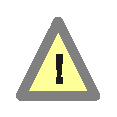
\includegraphics[width=0.6\textwidth]{../../_common/fig/symbols_warning.eps}   
\end{minipage}
\begin{minipage}{0.8\textwidth}
On Windows systems, you need to use the forward slash (\verb!/!) instead of the usual back-slash (\verb!\!) to separate directory names in the value of the environment variables listed in \tabref{tab:install:env:folders}. For example, if one of your \software{echse} standard folders is \verb!d:\modeling\echse_generic!, the proper value of \verb!ECHSE_GENERIC! would be \verb!d:/modeling/echse_generic!. Disregard of this will cause problems during the compilation of model engines.
\end{minipage} \\

\begin{minipage}{0.15\textwidth}
  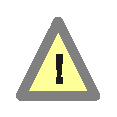
\includegraphics[width=0.6\textwidth]{../../_common/fig/symbols_warning.eps}   
\end{minipage}
\begin{minipage}{0.8\textwidth}
There must be no white space characters in the names of the \software{echse} standard folders. The existence of such characters (at any position) would break the functionality of some scripts. If you care for readability, use the \verb!_! character instead of white space, \ie{} use \verb!d:/my_files/echse_generic! instead of \verb!d:/my files/echse_generic!, for example. Disregard of this will cause problems during the compilation of model engines.
\end{minipage} \\

If you ever move one (or all) of the \software{echse} standard folder(s), the variables listed in \tabref{tab:install:env:folders} need to be updated to reflect the new location(s). If you follow the recommendations in \secref{sec:install:env:path}, no additional work is necessary.

\subsection{Adjusting the PATH variable} \label{sec:install:env:path}

Some sub-directories of the \software{echse} standard folders contain executable files (binaries and shell scripts). This is true in particular for the two folders \verb!echse_engines/bin! (\figref{fig:install:folders:engines}) and \verb!echse_generic/scripts! (\figref{fig:install:folders:generic}). It is recommended to add these two folders to the \verb!PATH! environment variable. Only then you will be able to run \software{echse}-based model engines as well as code generation and build scripts from any terminal without typing full path names.

It is strongly recommended that you make use of the already-defined environment variables \verb!ECHSE_ENGINES! and \verb!ECHSE_GENERIC! when adding these folders to \verb!PATH!. Then you can move the \software{echse} standard folders without updating \verb!PATH! again. For example, Linux users should could add the following line to their shell initialization file (see also \appref{chap:appendix:envVars}):

\begin{lstlisting}[style=shell]
  export PATH=$PATH:$ECHSE_ENGINES/bin:$ECHSE_GENERIC/scripts
\end{lstlisting}

Windows users need to adjust the settings in an equivalent way using the control panel. For example, the variable \verb!PATH! could have a contents similar to this one:
\begin{lstlisting}[style=shell]
  c:\mingw\bin;
  c:\mingw\msys\1.0\bin;
  c:\program files\R\R-2.15.2\bin;
  %ECHSE_GENERIC%\scripts;
  %ECHSE_ENGINES%\bin
\end{lstlisting}

Note that, to make this work, the \verb!PATH! variable being set must be of the same category as the referenced variables \verb!ECHSE_GENERIC! and \verb!ECHSE_ENGINES!. This is due to the fact that a \emph{user}-variable cannot be referenced in the definition of a \emph{system}-variable and vice versa. Therefore, users without administrator privileges usually need to define a user-variable \verb!PATH! in addition to the existing system-variable with that name.

%%%%%%%%%%%%%%%%%%%%%%%%%%%%%%%%%%%%%%%%%%%%%%%%%%%%%%%%%%%%%%%%%%%%%%%%%%%%%%
%%%%%%%%%%%%%%%%%%%%%%%%%%%%%%%%%%%%%%%%%%%%%%%%%%%%%%%%%%%%%%%%%%%%%%%%%%%%%%

\section{Building a model engine} \label{sec:install:build}

\subsection{Pre-requisites}

To be successsful, you should have read the sections \secsref{sec:install:folders}, \ref{sec:install:env}, and \ref{sec:install:software}. It is recommended that you perform some basic checks at a terminal prompt to make sure that the environment variable(s) are defined as intended and that the required software works properly.

\subsection{Run the code generator}
The code generator must be run from a shell prompt. On a Linux system, type the command \verb!echse_generate! followed by a space and the name of the model engine for which code is to be generated.

\medskip
\begin{minipage}{0.3\textwidth}
  Example:
\end{minipage}
\begin{minipage}{0.6\textwidth}
\begin{lstlisting}[style=shell]
  david@falkenstein:~$ echse_generate myEngine
\end{lstlisting}
\end{minipage}

On a Windows system, use the command  \verb!echse_generate_win.bat! instead of \verb!echse_generate!.

\medskip
\begin{minipage}{0.3\textwidth}
  Example:
\end{minipage}
\begin{minipage}{0.6\textwidth}
\begin{lstlisting}[style=shell]
  d:\> echse_generate_win.bat myEngine
\end{lstlisting}
\end{minipage}

\medskip
To make the commands work at any prompt, the folder \verb!echse_generic/scripts! (\figref{fig:install:folders:generic}) must be part of the \verb!PATH! variable (see \secref{sec:install:env:path}).

The scripts provide some basic error checking. In most cases, you should be able to fix the problem yourself. Note that you can only generate code for model engines that have already been designed (by declaring the classes).

\subsection{Run the build script}
The build script must be run from a shell prompt. On a Linux system, type the command \verb!echse_build! followed by a space and the name of the model engine. If want to skip the re-build of the static C++ library in order to speed up the compilation, you can set the second argument to 'n' (see example below). Use this option only if the library was just updated and note the warnings below.

\medskip
\begin{minipage}{0.3\textwidth}
  Examples:
\end{minipage}
\begin{minipage}{0.6\textwidth}
\begin{lstlisting}[style=shell]
  david@falkenstein:~$ echse_build myEngine
  david@falkenstein:~$ echse_build myEngine n
\end{lstlisting}
\end{minipage}

On a Windows system, use the command  \verb!echse_build_win.bat! instead of \verb!echse_build!.

\medskip
\begin{minipage}{0.3\textwidth}
  Examples:
\end{minipage}
\begin{minipage}{0.6\textwidth}
\begin{lstlisting}[style=shell]
  d:\> echse_build_win.bat myEngine
  d:\> echse_build_win.bat myEngine n
\end{lstlisting}
\end{minipage}

\medskip
To make the commands work at any prompt, the folder \verb!echse_generic/scripts! (\figref{fig:install:folders:generic}) must be part of the \verb!PATH! variable (see \secref{sec:install:env:path}).

\medskip
\begin{minipage}{0.15\textwidth}
  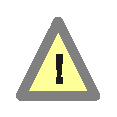
\includegraphics[width=0.6\textwidth]{../../_common/fig/symbols_warning.eps}   
\end{minipage}
\begin{minipage}{0.8\textwidth}
The C++ library \verb!libcpplib.a! is platform-specific, \ie{} you cannot re-use the file when switching between operating systems and/or compiler versions. Disregard of this may yield an executable with subtile bugs which are very hard to trace. Thus, the library must always be re-build after a new installation of the \software{echse} software and each time the C++ compiler is upgraded. The re-build should only be skipped if you run a sequence of attempts to build a model engine and compile time really matters.
\end{minipage} \\

The build scripts provide some basic error checking. If yout get rather lengthy error messages, possible several pages, this indicates a compiler problem. Please make sure that (1) you have the complete source code for the model engine you try to build, (2) the code generator ran without reporting errors, (3) the C++ library was re-build, and (4) the C++ compiler is properly installed.


%\chapter{Data types}  \label{app:datatypes}
\renewcommand{\tabdir}{appendix/datatypes/tab}
\renewcommand{\figdir}{appendix/datatypes/fig}

\section{Was ist der geeignete Array-Typ für die numerischen Rechnungen?}

Ausführungszeiten wurden mit unterschiedlichen Typen von Array getestet (verwendeter Testcode s.u.). Ergebnisse siehe \tabref{tab:arraytest}.

\begin{table*}[htbp]
  \caption{Mittlere Ausführungszeiten der Funktion in Sekunden bei verschiedenen
Compiler-Einstellungen (gcc (Ubuntu 4.4.1-4ubuntu9) 4.4.1). \label{tab:arraytest}}
  \begin{tabular}{lrrrr} \hline\hline
Compiler flag &    none &  -O &    -O2 &   -O4 \\ \hline
Vector &           1.4855 &0.661  &0.6225 &0.6115 \\
Valarray &         1.474  &0.6395 &0.6215 &0.6075 \\
Valarray(sclice) & 1.8875 &1.364  &0.63   &0.607 \\
C-Array &          1.3105 &0.6155 &0.628  &0.6105 \\ \hline\hline
\end{tabular}

\end{table*}

Fazit (für das getestete Beispiel):
\begin{itemize}
\item Bei Optimierung mit -O2 oder -O4 sind die Laufzeitunterschiede
  vernachlässigbar. Das einfachere Handling dürfte hier für die Ver-
  wendung des Typs valarray sprechen.
\item Wenn keine Optimierung eingeschaltet ist oder nur -O gesetzt ist, sind die
  C-arrays am effizientesten. Die Verwendung von valarray mit slices ist
  deutlich langsamer als die andern Varianten.
\end{itemize}

\begin{shaded}
  \scriptsize
  \lstinputlisting[style=c++]{\figdir/arraytest.cpp}
\end{shaded}


%%%%%%%%%%%%%%%%%%%%%%%%%%%%%%%%%%%%%%%%%%%%%%%%%%%%%%%%%%
%%%%%%%%%%%%%%%%%%%%% THE INDEX %%%%%%%%%%%%%%%%%%%%%%%%%%
%%%%%%%%%%%%%%%%%%%%%%%%%%%%%%%%%%%%%%%%%%%%%%%%%%%%%%%%%%

\clearpage
\fancyhead[LE,RO]{\bfseries\thepage}
\fancyhead[RE]{\bfseries Index}
\fancyhead[LO]{}
\addcontentsline{toc}{chapter}{Index}
\printindex

\end{document}
